% !TeX spellcheck = en_GB
% !TeX encoding = UTF-8
% !TeX program = xelatex
% TODO Change language to en_GB (recommended) or en_US for English documents
\documentclass[12pt,a4paper,oneside]{report}             % Single-side
%\documentclass[11pt,a4paper,twoside,openright]{report}  % Duplex
\usepackage{titlesec}
\usepackage{wrapfig}
\titleformat{\chapter}[hang]{\Huge\bfseries}{\thechapter{ }}{0pt}{\Huge\bfseries}
% thanks to http://tex.stackexchange.com/a/47579/71109
\usepackage{ifxetex}
\usepackage{ifluatex}
\newif\ifxetexorluatex % a new conditional starts as false
\ifnum 0\ifxetex 1\fi\ifluatex 1\fi>0
   \xetexorluatextrue
\fi

\ifxetexorluatex
  \usepackage{fontspec}
\else
  \usepackage[T1]{fontenc}
  \usepackage[utf8]{inputenc}
  \usepackage[lighttt]{lmodern}
\fi

\usepackage[english,magyar]{babel} % Alapértelmezés szerint utoljára definiált nyelv lesz aktív, de később külön beállítjuk az aktív nyelvet.

%\usepackage{cmap}
\usepackage{amsfonts,amsmath,amssymb} % Mathematical symbols.
%\usepackage[ruled,boxed,resetcount,linesnumbered]{algorithm2e} % For pseudocodes. % beware: this is not compatible with LuaLaTeX, see http://tex.stackexchange.com/questions/34814/lualatex-and-algorithm2e
\usepackage{booktabs} % For publication quality tables for LaTeX
\usepackage{graphicx}


%\usepackage{fancyhdr}
%\usepackage{lastpage}
\usepackage{float}
\usepackage{anysize}
\usepackage{wrapfig}
%\usepackage{sectsty}
\usepackage{setspace} % For setting line spacing

\PassOptionsToPackage{hyphens}{url}\usepackage{hyperref}
\usepackage{xcolor}
\usepackage{listings} % For source code snippets.

\usepackage[amsmath,thmmarks]{ntheorem} % Theorem-like environments.

\usepackage[hang]{caption}

\singlespacing

\newcommand{\sectionbreak}{\clearpage}

\newcommand{\selecthungarian}{
	\selectlanguage{magyar}
	\setlength{\parindent}{2em}
	\setlength{\parskip}{0em}
	\frenchspacing
}

\newcommand{\selectenglish}{
	\selectlanguage{english}
	\setlength{\parindent}{0em}
	\setlength{\parskip}{0.5em}
	\nonfrenchspacing
	\renewcommand{\figureautorefname}{Figure}
	\renewcommand{\tableautorefname}{Table}
	\renewcommand{\partautorefname}{Part}
	\renewcommand{\chapterautorefname}{Chapter}
	\renewcommand{\sectionautorefname}{Section}
	\renewcommand{\subsectionautorefname}{Section}
	\renewcommand{\subsubsectionautorefname}{Section}
}

\usepackage[numbers]{natbib}
\usepackage{xspace}

\usepackage{longtable}
%TODO Set the main variables
\newcommand{\vikszerzoVezeteknev}{Maidics}
\newcommand{\vikszerzoKeresztnev}{Barnabas}

\newcommand{\vikkonzulensAMegszolitas}{}
\newcommand{\vikkonzulensAVezeteknev}{Vary}
\newcommand{\vikkonzulensAKeresztnev}{Peter}

\newcommand{\vikkonzulensBMegszolitas}{PhD~}
\newcommand{\vikkonzulensBVezeteknev}{Dudas}
\newcommand{\vikkonzulensBKeresztnev}{Akos}

\newcommand{\vikkonzulensCMegszolitas}{}
\newcommand{\vikkonzulensCVezeteknev}{}
\newcommand{\vikkonzulensCKeresztnev}{}

\newcommand{\vikcim}{Analyze and optimize the performance of Hive} % Cím
\newcommand{\viktanszek}{Department of Automation and Applied Informatics} % Tanszék
\newcommand{\vikdoktipus}{\bsc} % Dokumentum típusa (\bsc vagy \msc)
\newcommand{\vikmunkatipusat}{szakdolgozatot} % a "hallgató nyilatkozat" részhez: szakdolgozatot vagy diplomatervet

\newcommand{\myparagraph}[1]{\paragraph{#1}\mbox{}\\}


\input{include/tdk-variables}
\newcommand{\szerzoMeta}{\vikszerzoVezeteknev{} \vikszerzoKeresztnev} % egy szerző esetén
%\newcommand{\szerzoMeta}{\vikszerzoVezeteknev{} \vikszerzoKeresztnev, \tdkszerzoB} % két szerző esetén




%TODO Language configuration -- choose one
% Beállítások magyar nyelvű dolgozathoz
%\input{include/thesis-hu}
% Settings for English documents
%--------------------------------------------------------------------------------------
% Elnevezések
%--------------------------------------------------------------------------------------
\newcommand{\bme}{Budapest University of Technology and Economics}
\newcommand{\vik}{Faculty of Electrical Engineering and Informatics}

\newcommand{\bmemit}{Department of Measurement and Information Systems}

\newcommand{\keszitette}{Author}
\newcommand{\konzulens}{Advisors}

\newcommand{\bsc}{Bachelor's Thesis}
\newcommand{\msc}{Master's Thesis}
\newcommand{\tdk}{Scientific Students' Association Report}
\newcommand{\bsconlab}{BSc Project Laboratory}
\newcommand{\msconlabi}{MSc Project Laboratory 1}
\newcommand{\msconlabii}{MSc Project Laboratory 2}

\newcommand{\pelda}{Example}
\newcommand{\definicio}{Definition}
\newcommand{\tetel}{Theorem}

\newcommand{\bevezetes}{Introduction}
\newcommand{\koszonetnyilvanitas}{Acknowledgements - Köszönetnyilvánítás}
\newcommand{\fuggelek}{Appendix}

% Optional custom titles
%\addto\captionsenglish{%
%\renewcommand*{\listfigurename}{Your list of figures title}
%\renewcommand*{\listtablename}{Your list of tables title}
%\renewcommand*{\bibname}{Your bibliography title}
%}

\newcommand{\szerzo}{\vikszerzoKeresztnev{} \vikszerzoVezeteknev}
\newcommand{\vikkonzulensA}{\vikkonzulensAMegszolitas\vikkonzulensAKeresztnev{} \vikkonzulensAVezeteknev}
\newcommand{\vikkonzulensB}{\vikkonzulensBKeresztnev{} \vikkonzulensBVezeteknev, \vikkonzulensBMegszolitas}
\newcommand{\vikkonzulensC}{\vikkonzulensCMegszolitas\vikkonzulensCKeresztnev{} \vikkonzulensCVezeteknev}

\newcommand{\selectthesislanguage}{\selectenglish}

\bibliographystyle{plainnat}

\newcommand{\ie}{i.e.\@\xspace}
\newcommand{\Ie}{I.e.\@\xspace}
\newcommand{\eg}{e.g.\@\xspace}
\newcommand{\Eg}{E.g.\@\xspace}
\newcommand{\etal}{et al.\@\xspace}
\newcommand{\etc}{etc.\@\xspace}
\newcommand{\vs}{vs.\@\xspace}
\newcommand{\viz}{viz.\@\xspace} % videlicet
	\newcommand{\cf}{cf.\@\xspace} % confer
\newcommand{\Cf}{Cf.\@\xspace}
\newcommand{\wrt}{w.r.t.\@\xspace} % with respect to
\newcommand{\approximately}{approx.\xspace}

\newcommand{\appendixnumber}{1}  % a fofejezet-szamlalo az angol ABC 1. betuje (A) lesz

\linespread{1.25}
\input{include/preamble}
%--------------------------------------------------------------------------------------
% Table of contents and the main text
%--------------------------------------------------------------------------------------
\begin{document}

%TODO These define guidelines -- remove these
%~~~~~~~~~~~~~~~~~~~~~~~~~~~~~~~~~~~~~~~~~~~~~~~~~~~~~~~~~~~~~~~~~~~~~~~~~~~~~~~~~~~~~~
%\include{include/guideline}
%\include{include/project}

\selectthesislanguage

%TODO Titlepage -- choose one from below
%~~~~~~~~~~~~~~~~~~~~~~~~~~~~~~~~~~~~~~~~~~~~~~~~~~~~~~~~~~~~~~~~~~~~~~~~~~~~~~~~~~~~~~
\include{include/titlepage}		   % Szakdolgozat/Diplomaterv címlap
%\include{include/titlepage-tdk}	% TDK címlap
%\include{include/titlepage-otdk}   % OTDK címlap


% Table of Contents
%~~~~~~~~~~~~~~~~~~~~~~~~~~~~~~~~~~~~~~~~~~~~~~~~~~~~~~~~~~~~~~~~~~~~~~~~~~~~~~~~~~~~~~
\tableofcontents\vfill


% Declaration and Abstract
%~~~~~~~~~~~~~~~~~~~~~~~~~~~~~~~~~~~~~~~~~~~~~~~~~~~~~~~~~~~~~~~~~~~~~~~~~~~~~~~~~~~~~~
\include{include/declaration} %TODO Hallgatói nyilatkozat -- TDK és OTDK esetén törlendő!
%TODO Abstract megírása
\pagenumbering{roman}
\setcounter{page}{1}

\selecthungarian

%----------------------------------------------------------------------------
% Abstract in Hungarian
%----------------------------------------------------------------------------
\chapter*{Kivonat}\addcontentsline{toc}{chapter}{Kivonat}

Apache Hive eredetileg a Facebook által készített nyílt forráskódú, adattárház platform. Célja, hogy megkönnyítse az adatelemzők munkáját azzal, hogy bevezetett egy, az SQL-hez hasonló nyelvet, a HiveQL-t. Hive bemenete egy HiveQL lekérdezés, amit feldolgoz, szemantikailag elemzi, majd amennyiben lehetséges optimalizálja különböző optimalizációs stratégiákat felhasználva. Végezetül generál egy Hadoop feladatot, amit az végre tud hajtani. Hive nem csak Hadoopot tud használni végrehajtó motortként, támogatja az Apache Spark és Apache Tez használatát is. 

Bizonyos körülmények között Hive memória problémákkal küzd. HiveServer2 az egyik fő komponense, gyakran összeomlik Out Of Memory (OOM) hibaüzenettel. Jelen dolgozattal a célom, hogy felépítsek egy alapvető modellt, melnyek segítségével megtudjuk miért és a lekérdezés életciklusában mikor növekszik jelentősen a memóriahasználat, valamint memória problémákat találjak és amennyiben lehetséges ezekre megoldási javaslatot adjak.

A model építéshez segítségül létrehoztam egy eszközt, melynek használatával információkat tudok kinyerni a memóriahasználattal kapcsolatban és heap mintákat (heap dump) tudok generálni automatikusan a lekérdezés élete során, későbbi elemzés céljából. Az említett és más memória elemző eszközök segítségével azonosítottam két problémát, amik a heap memóriát jelentősen tudják növelni. Az egyik probléma HDFS-ből származik (Hadoop elosztott fájlrendszere), ezért Hadoop kód megértése és módosítása is szükségessé vált. Mindkét memória problémára, létrehoztam egy megoldási javaslatot, és csináltam egy lehetséges implementációt ami segíthet megszabadulni a memória problémától. Mindkét javítás alapos tesztelést igényelt: lokális, egyszerű teljesítmény tesztekre és skálázható adatközpont klaszteren végrehajtott benchmark tesztekre is szükség volt. Az azonosított problémák vizsgálata jelenleg is folyamatban van. A HDFS javításom előidézhet nehezen detektálható, váratlan CPU problémákat, ezért annak eldöntésére hogy a kompromisszum előnyös lesz, nagyon alapos tesztelés szükséges.


\vfill
\selectenglish


%----------------------------------------------------------------------------
% Abstract in English
%----------------------------------------------------------------------------
\chapter*{Abstract}\addcontentsline{toc}{chapter}{Abstract}
Apache Hive is an open source data warehouse platform originally built on top of Hadoop by Facebook. Hive makes the work of data scientists easier by introducing a language similar to SQL, called HiveQL. Hive takes query written in HiveQL, does parsing and analyzing and if possible, optimizes the query using several optimization strategies. Finally, it creates a Hadoop job and executes it on the platform. Currently, not only Hadoop can be used as an execution engine, Hive can even work on Apache Spark or Apache Tez. 

Hive faces memory problems under certain circumstances. HiveServer2 is one of the main components of Hive and often crashes due to Out Of Memory (OOM) error. In my thesis, I aim to build a basic model, to understand why and when the memory usage of HiveServer2 rises and find memory-related problems or wastes.

To be able to build a model, I created a basic tool for getting memory information and generating heap dumps automatically during the life of a query. With the help of my tool and other memory analysis tools, I generated and analyzed many heap dumps. I was able to identify two issues that can cause big pressure on heap memory. One of the issues is introduced by HDFS (distributed file system of Hadoop), therefore touching Hadoop was also necessary. For both memory issues, I suggested a possible solution and created an implementation, that can help get rid of the memory overheads. These patches required multiple tests: local, simple performance testing and scalable benchmarking on a data center cluster. The issues identified are still ongoing and currently under investigation since the HDFS patch might introduce unexpected CPU overhead which are hard to detect so deciding whether this tradeoff is negligible requires a thorough testing. 

\vfill
\selectthesislanguage

\newcounter{romanPage}
\setcounter{romanPage}{\value{page}}
\stepcounter{romanPage}    %TODO Összefoglaló -- TDK és OTDK esetén nem kötelező


% The main part of the thesis
%~~~~~~~~~~~~~~~~~~~~~~~~~~~~~~~~~~~~~~~~~~~~~~~~~~~~~~~~~~~~~~~~~~~~~~~~~~~~~~~~~~~~~~
\pagenumbering{arabic}
\setlength{\parindent}{1.5 cm} % Default is 15pt.
%TODO import your own content
%----------------------------------------------------------------------------
\chapter{\bevezetes}
%----------------------------------------------------------------------------


The digital era has led to large amounts of data being amassed by companies every day. Data comes from multiple sources: sensors, sales data, communication systems, logging of system events \etc. According to Forbes \cite{Forbes} 2.5 quintillion bytes of data is created each day. That means 2.5 million Terabytes per day. Bigger corporations can easily create hundreds of Terabytes daily. We need a new solution to process this amount of data. The traditional relational databases (RDBMS) can deal only with Gigabytes. Hadoop provides a software framework to scale up our system for storing, processing and analyzing big data.

In this chapter, I will write about the basics of Hadoop architecture, why Hive was created on top of it and the performance issues it faces.

\section{Hadoop basics}
Apache Hadoop is an open source distributed framework for managing, processing  and storing a huge amount of data in clustered systems built from commodity hardware. All modules in Hadoop were designed with an assumption that hardware failures are frequent and should be automatically handled by the framework. One of the most important characteristics of Hadoop is that it partitions the data and computation across many hosts and executes computation in parallel close to the data it uses.  \cite{Hadoop-wiki}

The base of the Hadoop framework contains the following modules:
\begin{itemize}
	\item HDFS - Hadoop Distributed File System: designed to store large data sets reliably and stream those at high bandwidth to user applications.
	\item Hadoop MapReduce: an implementation of the MapReduce programming model for large data processing
	\item YARN - Yet Another Resource Negotiator: a resource management and job scheduling technology
	\item Hadoop Common: contains libraries and utilities for other Hadoop modules
\end{itemize}
\iffalse\subsection{Hadoop \vs traditional databases}
Traditional databases cannot be used when we want to process and store big data. Main differences between Hadoop and traditional RDBMS \cite{Hadoop-vs-RDBMS}:
\begin{itemize}
	\item \textbf{Data Volume}: RDBMS works better when data volume is low (Gigabytes). However, when data size is huge (Terabytes-Petabytes) traditional databases fail. Users have to pick another solution for the problem. Hadoop can easily handle this amount of data so it became the number one big data platform.
	\item \textbf{Data Variety}: It means what type of data we want to process. Hadoop is able to store and process either structured, semi-structured or unstructured data. Even though  it is mostly used for huge amounts of unstructured data. 
	In contrast, traditional RDBMS can only be used to manage structured or semi-structured data. 
	\item \textbf{Scalability}: RDBMS provides vertical scalability. We can add more resources, memory or CPU to a machine in the cluster. Whereas Hadoop scales horizontally which means we can add more machines to an existing cluster. As a result of this, Hadoop becomes fault tolerant. We can easily recover data in case of a failure.
	\item \textbf{Data Processing}: Apache Hadoop supports OLAP (Online Analytical Processing), which involves very complex queries and aggregations. The database design is de-normalized, having fewer tables. On the other hand, RDBMS supports OLTP (Online Transaction Processing), which involves fast query processing. The database design is normalized and contains large numbers of tables.
\end{itemize}\fi
\subsection{HDFS - Hadoop Distributed File System}
HDFS is the file system of Hadoop. It stores file system metadata and application data separately. The dedicated server that stores metadata is the NameNode. Application data is stored on other servers (DataNodes). These servers are connected and they communicate using TCP-based protocols \cite{Shvachko:2010:HDF:1913798.1914427}. 

The file system is based on the following goals and principles \cite{HDFS-docs}:
\begin{itemize}
	\item \textbf{Hardware failure}: Hardware failures should be considered as normal, rather than an exception. An HDFS instance consists of hundreds or thousands of components so this means that some of them will always be non-functional. Therefore, fault detection and automatic recovery is a must.
	\item \textbf{Streaming Data Access}: HDFS was designed for batch processing rather than interactive use. Therefore, HDFS users need streaming access to their data. This means that high throughput is more important than low latency.
	\item \textbf{Large Data Sets}: The size of a typical HDFS file is gigabytes to terabytes. Thus, the file system is tuned to support large files. 
	\item \textbf{Simple Coherency}: HDFS follows WORM (Write-Once-Read-Many) model. A file, once written should not be changed except for appends and truncates.  This assumption simplifies data coherency issues. A MapReduce application fits perfectly for this model.
	\item \textbf{Moving computation}: A computation is much more efficient if it is executed near the data it operates on. It is especially true for big data. 
	\item \textbf{Portability}: HDFS was designed to port from one platform to another with ease. 
\end{itemize}
\subsubsection*{NameNode}
NameNode keeps the directory tree of all files in the file system and tracks where data is kept across the cluster, it does not store the files. Clients talk to the NameNode whenever they want to locate a file. The NameNode's response is a list of relevant DataNode servers where the data is available. 

As a result of this approach, the NameNode is a Single Point of Failure in the HDFS cluster. Whenever the NameNode goes down, the file system becomes offline.
\begin{figure}[H]
	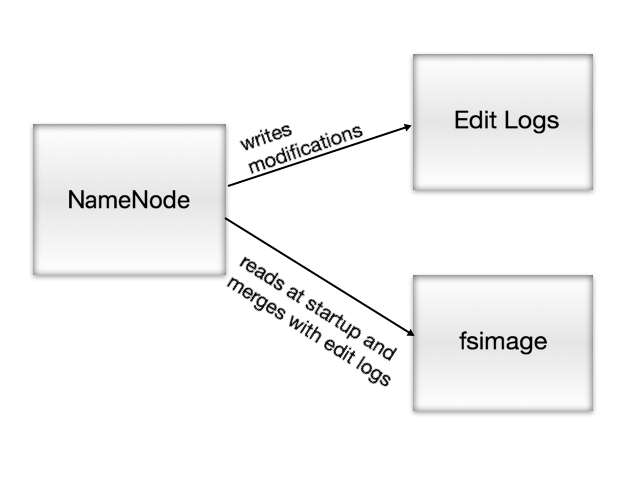
\includegraphics[width=80mm, keepaspectratio]{figures/namenode_problem.png}
	\centering
	\caption*{Problem with NameNode}
\end{figure}
The image shows how NameNode stores information \cite{Secondary-NameNode}. There are two different files:
\begin{itemize}
	\item edit logs: the changes made to the file system after the NameNode started
	\item fsimage: a snapshot of the file system when the NameNode started
\end{itemize}
In production clusters, the NameNode restarts are very rare. That means edit logs can grow large therefore in case of a crash we will lose a huge amount of metadata since the fsimage is very old.

The Secondary NameNode helps to solve this issue. It is responsible for merging the edit logs with fsimage. It collects edit logs on a regular basis and applies them to the fsimage. NameNode will use this fsimage in case of a crash and it can also be used to reduce the startup time of the NameNode.
It is important to remember that the Secondary NameNode is not a real backup NameNode it only merges the edits into the fsimage. 

\begin{figure}[H]
	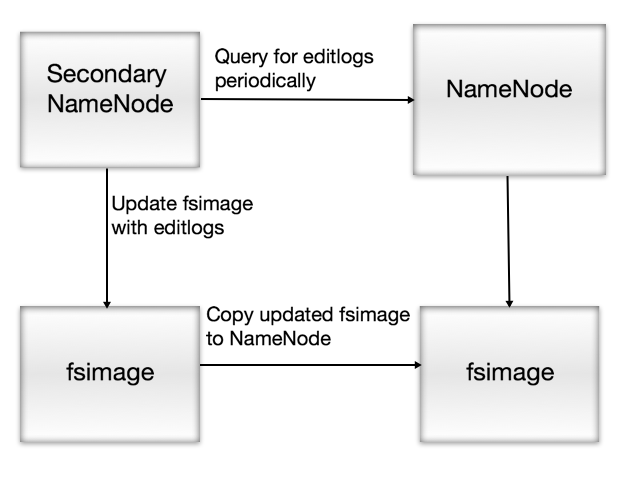
\includegraphics[width=80mm, keepaspectratio]{figures/secondary_namenode.png}
	\centering
	\caption*{Solution using the Secondary NameNode}
\end{figure}

\subsubsection*{DataNodes \cite{Shvachko:2010:HDF:1913798.1914427}}
On a DataNode, a block is represented by two files in the native file system. The first contains the data itself, the second is the metadata.

On startup, the DataNodes connect to the NameNode and perform a handshake. This will verify the namespace ID and software version of the DataNodes. If one of them does not match with the NameNode's value, the DataNode automatically shuts down. After a successful handshake, the DataNode registers with the NameNode. DataNode will store it's internal identifier. If restart occurs the DataNodes will be recognizable with the ID, even if they get a different IP address or port. After the ID is registered to the NameNode the it will never change. 

 When a DataNode is registered it sends a block report immediately. It contains block id, generation stamp and the length of each block the DataNode hosts. To provide up-to-date information to the NameNode reports are sent every hour. 

DataNodes send heartbeats to the NameNode. It ensures the NameNode that the DataNode is operating and block replicas of the server are available. If the NameNode does not receive a heartbeat from a DataNode it will consider the node to be out of service. The default heartbeat interval is three seconds.

\subsubsection*{HDFS Client \cite{Shvachko:2010:HDF:1913798.1914427}}
User applications can access the file system using the HDFS client which exports the HDFS file system interface. HDFS supports operations similar to a traditional file system: read, write, create or delete files and create or delete directories. The user can refer to files or directories using paths in the namespace.

When someone reads a file, HDFS Client asks the NameNode for the list of DataNodes that host replicas of the blocks of the file. Then it will directly contact the DataNode and request the desired block.

\begin{figure}[H]
	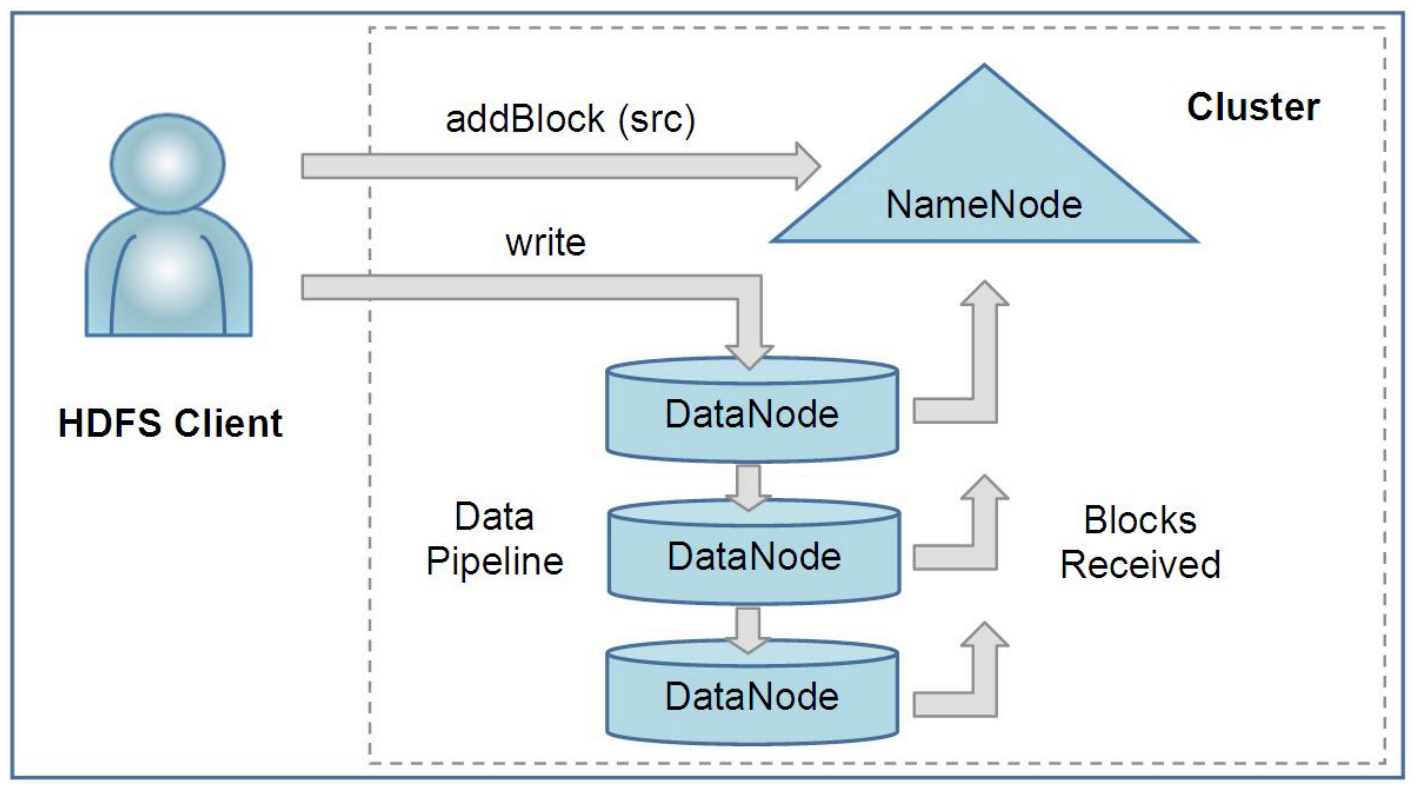
\includegraphics[width=100mm, keepaspectratio]{figures/hdfs_client.png}
	\centering
	\caption*{HDFS file writing}
\end{figure}
The client creates a new file by giving its path to the NameNode. For each block, the NameNode will return a list of DataNodes to place the replicas. The client pipelines data to the given DataNodes, and they will confirm the creation of the block to the NameNode.
\subsection{MapReduce}
MapReduce is a programming model for processing data sets. Users specify two functions \cite{Dean:2004:MSD:1251254.1251264}:
\begin{itemize}
	\item map function: processes a key-value pair to generate a set of key-value pairs
	\item reduce function: merges the intermediate values associated with the same key
\end{itemize}

Programs written in MapReduce are automatically executed parallelly on large clusters. Using this, programmers with no experience in parallel programming and distributed systems can utilize the available resources on the cluster.
\paragraph{Example \cite{MapReduce-example}}
This example shows how MapReduce handles the problem of counting words. We have the following list of words: 
\begin{center}
	\textbf{Dear, Bear, River, Car, Car, River, Deer, Car, Bear}
\end{center}

\begin{figure}[H]
	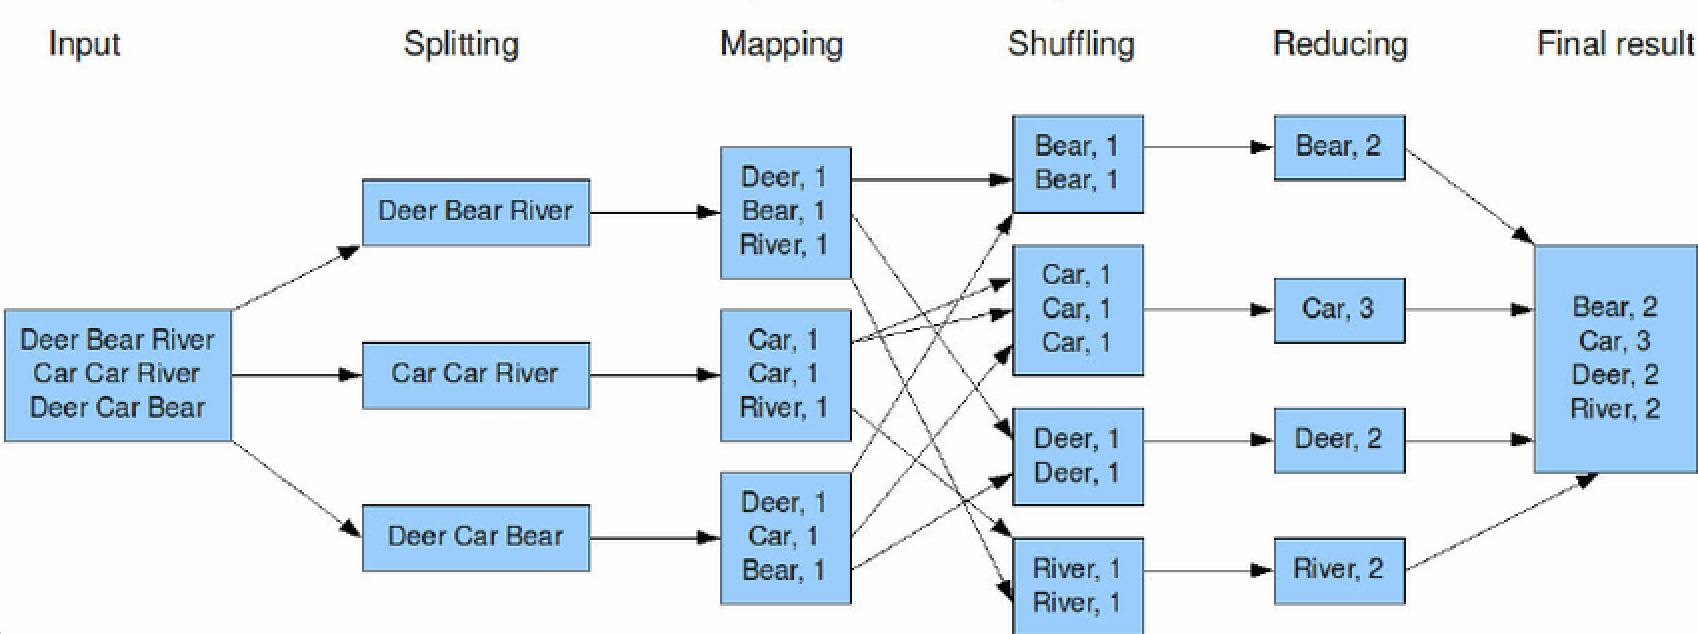
\includegraphics[width=150mm, keepaspectratio]{figures/MapReduce_Example.png}
	\caption*{The MapReduce word count process \cite{MapReduce-example-figure}}
	\centering
\end{figure}
\begin{itemize}
	\item \textbf{Splitting}: the first step is dividing the input into splits. This will distribute the work among the Map nodes.
	\item \textbf{Mapping}: tokenize the words in each mapper and giving a value of 1 for each word, since every word in itself will occur once.
	\item \textbf{Shuffling}: partition takes place with shuffling and sorting: this way pairs with the same key will be sent to the same reducer.
	\item \textbf{Reducing}: a reducer gets the list of pairs and counts the number of ones in this list.
\end{itemize}

\subsubsection*{Advantages of MapReduce \cite{MapReduce-example}}
\paragraph{Parallel processing}
In MapReduce we divide the job among multiple nodes, so they can work on their part of the data parallelly. This way the data processing is done by multiple machines instead of one, so the time is significantly reduced.
\paragraph{Data locality}
In Hadoop MapReduce, instead of moving data into the processing unit, we move the processing unit to the data. The traditional approach has its limit when it comes to processing big data. Moving huge data is costly: network issues can occur and the master node (where data is stored) can get overloaded and may fail. 

However, the MapReduce approach is very cost efficient, since all the nodes are working simultaneously on their part of the data and there is no chance of a node getting overloaded.

Using Hadoop we just need to provide the map and reduce functions, the rest is done by the framework.  The word count example would look like the following in Java:
\paragraph{Map}\mbox{}\\
\begin{lstlisting}[language=Java]
	public void map(LongWritable key, Text value, Context context) throws IOException,InterruptedException {
		String line = value.toString();
		StringTokenizer tokenizer = new StringTokenizer(line);
		while (tokenizer.hasMoreTokens()) {
			value.set(tokenizer.nextToken());
			context.write(value, new IntWritable(1));
		}
	}
\end{lstlisting}
The input and output of the Mapper is a key/value pair. 

Input:
\begin{itemize}
	\item Key: the offset of each line
	\item Value: each line
\end{itemize}

Output:
\begin{itemize}
	\item Key: the tokenized words
	\item Value: the hardcoded value 1
\end{itemize}

\paragraph{Reduce}\mbox{}\\
\begin{lstlisting}
	public void reduce(Text key, Iterable<IntWritable> values,Context context) throws IOException,InterruptedException {
		int sum=0;
		for(IntWritable x: values) {
			sum+=x.get();
		}
		context.write(key, new IntWritable(sum));
	}
\end{lstlisting}
Both the input and output of the Reducer is a key/value pair. 

Input:
\begin{itemize}
	\item Key: unique words, generated after the sorting and shuffling phase
	\item Value: a list of integers corresponding to each keys
	\item \eg Bear, [1, 1]
\end{itemize}

Output:
\begin{itemize}
	\item Key: all the unique words in the input text file
	\item Value: number of occurrences for each unique word
	\item \eg  Bear, 2; Car, 3
\end{itemize}

The traditional way to execute MapReduce operations is that the users specify the Map and Reduce functions in Java. However, this approach has some problems:
\begin{itemize}
	\item it is not a high-level language for data processing
	\item data scientists do not understand Java. They came from the world of traditional databases, where SQL is used.
	\item even a simple problem (like word counting) resulted in hundreds of lines of code.
\end{itemize}

Although, the Hadoop MapReduce framework is written in Java, with the help of Streaming API we can create Map and Reduce functions in any languages.

MapReduce gives us a solution for many big data problems. However, for some scenarios, MapReduce is not the ideal choice: \eg real-time analysis. In Hadoop 1.0 we could not use components other than MapReduce (for example Apache Storm which is ideal for real-time computation). The desire for utilizing the potential provided by the distributed file system (HDFS) in other solutions has grown. YARN provides a solution to fulfill this claim.
\clearpage \subsection{Yarn \cite{YARN}}
\subsubsection*{Hadoop 1.0 resource management}
Previous to Hadoop 2.0, a single JobTracker had the responsibility to monitor the resources and distribute the MapReduce jobs for the DataNodes and monitor these jobs. 

In Hadoop 1.0 the MapReduce module was responsible for cluster resource management and data processing as well.

\begin{figure}[H]
	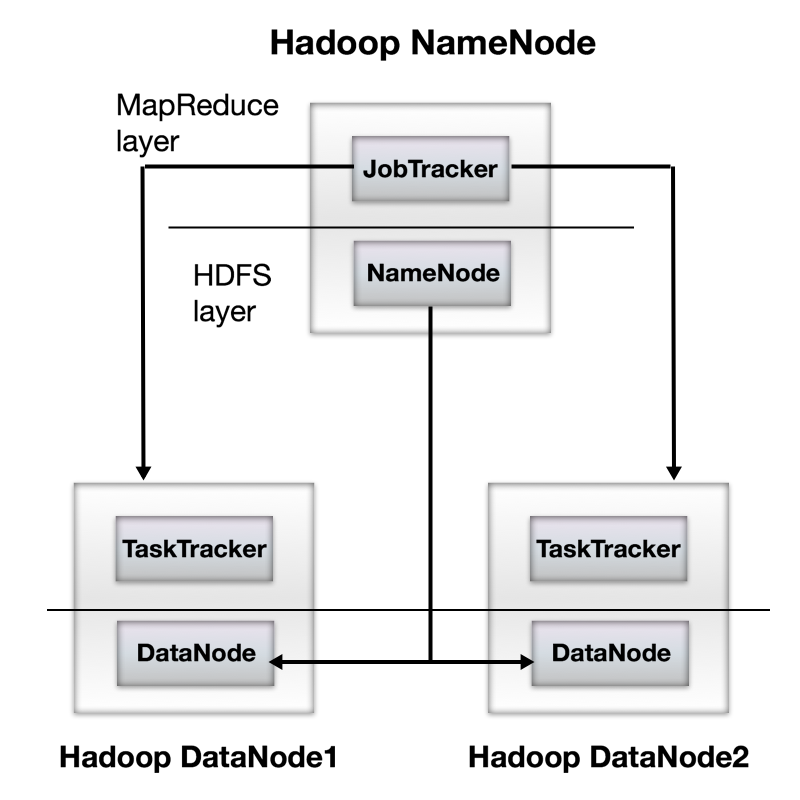
\includegraphics[width=100mm, keepaspectratio]{figures/hadoop10.png}
	\centering
	\caption*{Hadoop 1.0 architecture\cite{Hadoop1.0-problems}}
	\centering
\end{figure}

Resource management in Hadoop 1.0 \cite{Hadoop1.0}:

Clients submit jobs to the JobTracker which turns to the NameNode. It returns the location of the data. The JobTracker locates TaskTracker nodes with available slots close to the data and sends the job to the chosen TaskTracker nodes. After the job has started the JobTracker monitors the chosen TaskTracker nodes. If they do not send heartbeats frequently, they are deemed to have failed so the task will be scheduled on a different TaskTracker. The JobTracker gets a notification if a task fails. It decides what to do then: it may send the job to another TaskTracker, it can mark the record as something to avoid, or it may even put the TaskTracker to blacklist since it is unreliable. If the JobTracker sees that the task is finished, it will update its status. Clients poll the JobTracker for information.

The architecture of Hadoop 1.0 has many problems \cite{Hadoop1.0-problems}:
\begin{itemize}
	\item  It \textbf{limits scalability} since the JobTracker runs on a single machine doing multiple tasks it becomes a bottleneck: resource management, job and task scheduling, monitoring are done by the JobTracker.
	\item JobTracker is a \textbf{Single Point of Failure}. If it goes down, all the jobs are halted.
	\item In Hadoop 1.0 \textbf{JobTracker is tightly integrated with the MapReduce} module so only MapReduce applications can run on Hadoop. Although MapReduce is powerful enough to express many data analysis algorithms (mostly batch-driven data analysis), it is not always the optimal paradigm. It is often desirable to run other computation paradigms on Hadoop like real-time analysis and Message-Passing approach, \etc. Since HDFS makes it easy to store large amounts of data it is desirable to utilize this for other big data problems.
\end{itemize}

Developers recognized that splitting the responsibility to resource management and application monitoring has serious benefits. YARN is a re-architecture of Hadoop that allows multiple applications to run on the same platform. With YARN, applications run "in" Hadoop, instead of "on" Hadoop. This takes Hadoop beyond a batch processing application to a "data operating system" where HDFS is the file system and YARN is the operating system. 

\begin{figure}[H]
	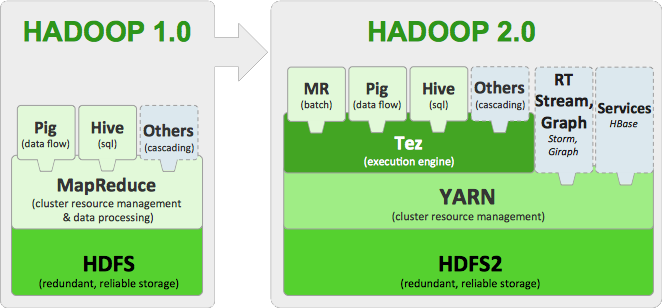
\includegraphics[width=100mm, keepaspectratio]{figures/hadoop10vs20.png}
	\centering
	\caption*{From Hadoop 1.0 to Hadoop 2.0}
	\centering
\end{figure}

The fundamental idea behind YARN is to split up the functionalities of resource management and job scheduling/monitoring. In YARN we have a global ResourceManager (RM) and ApplicationMaster (AM) for each application.

\textbf{ResourceManager} is responsible for distributing the resources among all the applications in the system. The \textbf{NodeManager} is a per-machine agent who monitors the resource usages (CPU, memory, network, disk) of the containers and reports them to the ResourceManager. 

The \textbf{ApplicationMaster} is framework specific, and its task is to ask the ResourceManager for resources when needed. It is also working with the NodeManager to execute and monitor tasks.

The ResourceManager is divided into two main components: Scheduler and ApplicationsManager.
\begin{itemize}
	\item The Scheduler is responsible for allocating resources to applications running in the cluster. It schedules based on the resource requirements of each application. The Scheduler does not perform monitoring or status tracking.
	\item The ApplicationsManager accepts job-submissions. It negotiates the first container for executing the application specific ApplicationMaster. It is also responsible for restarting the ApplicationMaster if it fails. 
\end{itemize}

\begin{figure}[H]
	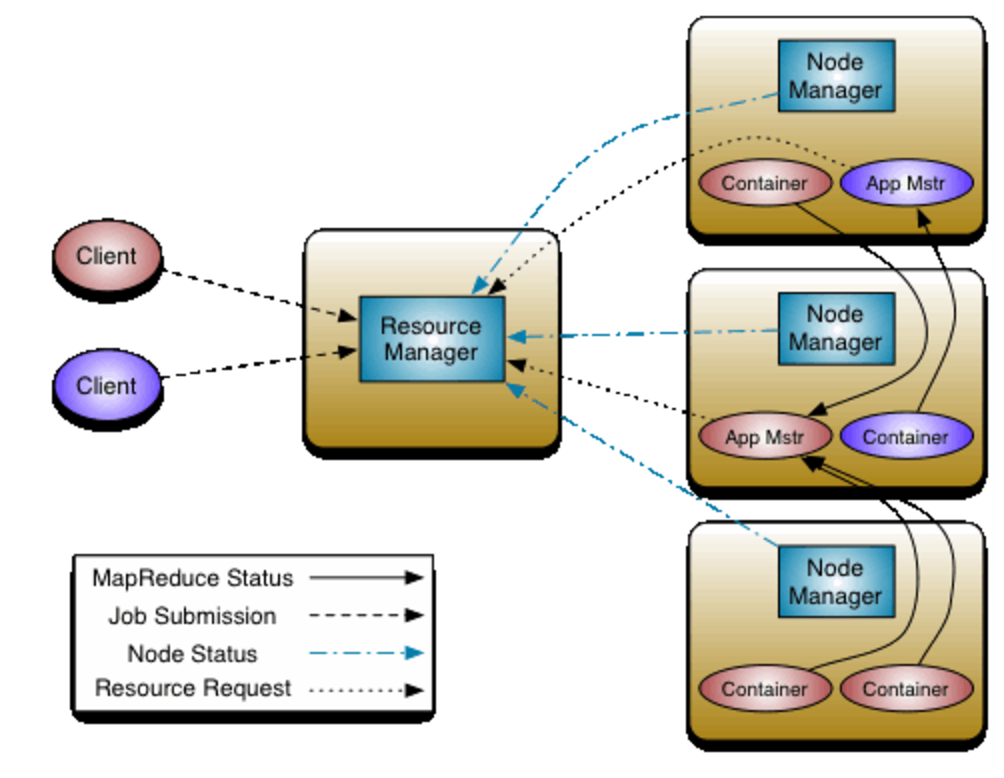
\includegraphics[width=120mm, keepaspectratio]{figures/yarn.png}
	\centering
	\caption*{Yarn architecture}
	\centering
\end{figure}

In summary, with YARN Hadoop is able to run applications that do not follow the MapReduce model since it decouples the resource management and scheduling capabilities of MapReduce. With the help of YARN, we can efficiently utilize the resources and can run multiple applications in Hadoop, all sharing a common resources.

\section{Apache Hive}
Hadoop is a popular implementation of the map-reduce model and used widely to process and store extremely large datasets. However, a map-reduce program is very low level and difficult to maintain or reuse. Data scientist come from a world, where SQL is the standard of data processing. Apache Hive gives us a data warehouse solution built on top of Hadoop to write SQL-like queries so we can utilize the advantage of a declarative language. The language similar to SQL is called HiveQL.

\subsection{Hive \vs RDBMS}
This section shows the main differences between Hive and traditional databases (\eg MySQL, Oracle, MS SQL \etc).

Hive supports SQL interface but it is not a full database. It follows WORM (Write Once Read Many) model while RDBMS is designed for Write and Read many times. Hive uses schema on read and traditional databases offer schema on write. Looking into Hive's approach, data is not validated until it is read. We can define multiple schemas to the same data and it provides a fast initial loading since the operation is just a copy and write. However the schema on read approach has some drawbacks. Schema check on write ensures that the data is not corrupt and it provides a better query performance because when reading data, schema checking is not needed. Hive is a better choice when the schema is not available at loading time since it can be added later dynamically. 

From Hive 0.13, Hive supports transactions \cite{Hive-transactions} and full ACID semantics at row level, but with many limitations. Previous to this, atomicity, consistency and durability were available and only at partition level. With introducing transactions Insert, Update and Delete keywords were added to HiveQL. 

The maximum data size allowed in a traditional RDBMS is 10's of Terabytes. However, Hive can easily handle Petabytes.

\subsubsection*{Conclusion}
Hive is a great choice if we want to analyze large unstructured, relatively static data sets, fast querying is not necessary and easy, low-cost scalability is required. RDBMS provides fast responses for analyzing data dynamically, but scalability and maximum data size are limited.

\subsection{Data storage}
Hive structure data in the following units  \cite{Hive-paper, Hive-data-units}:
\begin{itemize}
\item \textbf{Databases}: namespaces to avoid conflicts of table, partition or bucket names.
\item \textbf{Tables}: storage unit for data with the same schema. Tables maps to directories in HDFS.
\item \textbf{Partitions}: Tables can have many partition keys. These will determine how data is stored. In HDFS partitions map to subdirectories in the table's directory. This way we can speed up the analysis. Instead of running the query in the whole table, Hive will only run our query in the relevant partitions (see example below). Partition columns are virtual, which means they are not part of the data itself.
\item \textbf{Buckets}: Data can be divided into buckets based on the hash value of a column. These are helpful for efficiently sample data. Buckets are stored in files in the table's or partition's directory.
\end{itemize}

\subsubsection*{Example}
This example shows how Hive data units map to HDFS and and how partitioning tables can speed up queries.

Hive tables map to \texttt{<warehouse\_root\_directory>/table\_name} directory. As default, the warehouse root directory is /user/hive/warehouse. This can be changed with the corresponding hive configuration value.
\begin{lstlisting}
	CREATE TABLE test_table(c1 string, c2 int) 
		PARTITIONED BY (date string, hour int);
\end{lstlisting}
The above SQL statement will create a table with two columns and two partitions and it will be stored in  \texttt{/user/hive/warehouse/test\_table} directory in HDFS. For every distinct date and hour value, a partititon will exists. Although, the partition columns are not part of the data, they are stored in the table metadata. 

New partitions can be added either with the INSERT or the ALTER statement. These commands will create the corresponding HDFS directories: 

\texttt{/user/hive/warehouse/test\_table/date=2018-01-01/hour=12 and /user/hive/warehouse/test\_table/date=2018-01-02/hour=11}.

\begin{lstlisting}
	INSERT OVERWRITE TABLE
		test_table PARTITION(date='2018-01-01', hour=12)
	SELECT * FROM t;
	
	ALTER TABLE test_table
		ADD PARTITION(date='2018-01-02', hour=11);
\end{lstlisting}

Hive can use these information for pruning the directories to be scanned for query execution. 
\begin{lstlisting}
	SELECT * FROM test_table WHERE date='2018-01-01';
\end{lstlisting}
In case of this query, Hive will only scan the files in \texttt{/user/hive/warehouse/test\_table/date=2018-01-01} directory. Partitioning our data has significant impact on the time taken by queries.

Although, data in Hive is always in the corresponding directory (\texttt{<warehouse\_root\_directory>/table\_name}), Hive is able to query data stored in other locations in HDFS. In order to do this, we can create EXTERNAL tables as the following statement shows:
\begin{lstlisting}
	CREATE EXTERNAL TABLE test_external(c1 string, c2 int)
		LOCATION '/user/example_table/example_data';
\end{lstlisting}
Hive assumes that the external table in its internal format. The difference between an external and normal (managed by Hive) table is that the drop table command doesn't effect the data itself on an external table. However, on a normal table, it drops the associated data.

\subsection{Architecture}
The main components of Hive are the following \cite{Hive-paper}:
\begin{itemize}
	\item \textbf{Driver}: manages the lifecycle of a HiveQL query by creating a session for it. The driver also collects the result after the execution phase.
	\item  \textbf{MetaStore}: stores metadata about tables, columns or partitions. For example, it stores the table schema and location.
	\item \textbf{Compiler}: compiles the HiveQL statement and generates the execution plan using the partition and table metadata obtained from the MetaStore. First, it parses the query and does semantic analysis. Then converts it into AST (Abstract Syntax Tree) and after compatibility checking to a DAG of Map and Reduce tasks (if Hadoop MapReduce is the execution engine). 
	\item \textbf{Optimizer}: transformations are done to get an optimized DAG for better performance. It is an evolving component. In the earlier stage, only rule-based optimization was available which performed column pruning and predicate pushdown. Later, map-side join was introduced and several other join optimization, also cost-based optimization was added.
	\item \textbf{Execution Engine}: executes the plan created by the compiler. The plan is a DAG of stages. The engine manages the dependencies between these stages and executes them in the corresponding component. Hive is compatible with 3 execution engines: MapReduce, Apache TEZ and Spark which can run in Hadoop YARN.
	\item \textbf{HiveServer2}: a service that provides a thrift interface so clients can execute queries against Hive. Thrift is an RPC (Remote Call Procedure) framework for defining services for multiple languages.
	\item \textbf{Clients}: multiple clients are available to interact with Hive. Beeline (CLI), JDBC/ODBC, Python or Ruby client \etc.
\end{itemize}

\begin{figure}[H]
	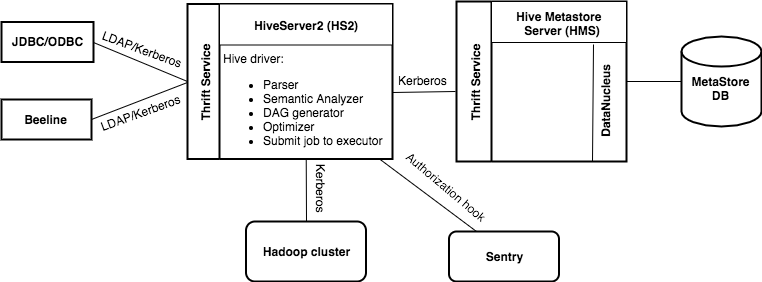
\includegraphics[width=150mm, keepaspectratio]{figures/Hive_architecture.png}
	\centering
	\caption*{Hive architecture}
\end{figure}

Clients can connect to HiveServer2 using its Thrift Service. HS2 supports authentication of the clients using Kerberos or LDAP authentication. Hive Metastore server also supports Kerberos authentication for Thrift clients.

Sentry is a role-based authorization module for Hadoop, so we can control the priviliges for authenticated users. Hive can use Sentry over an "authorization hook", which Sentry registers to Hive configuration file if secure cluster is enabled. 

HMS uses DataNucleus to persist metadata, so any relational database supported by it cal be used: it can be either embedded (\eg Derby) or remote (\eg MySQL) Metastore database.
\chapter{Apache Hadoop}
Apache Hadoop is an open source distributed framework for managing, processing and storing a huge amount of data in clustered systems built from commodity hardware. All modules in Hadoop were designed with an assumption that hardware failures are frequent and should be automatically handled by the framework. One of the most important characteristics of Hadoop is that it partitions the data and computation across many hosts and executes computation in parallel close to the data it uses.  \cite{Hadoop-wiki}

\noindent The base of the Hadoop framework contains the following modules:
\begin{itemize}
	\item HDFS - Hadoop Distributed File System: designed to store large data sets reliably and stream those at high bandwidth to user applications.
	\item Hadoop MapReduce: an implementation of the MapReduce programming model for large data processing
	\item YARN - Yet Another Resource Negotiator: a resource management and job scheduling technology
	\item Hadoop Common: contains libraries and utilities for other Hadoop modules
\end{itemize}

\section{HDFS - Hadoop Distributed File System}
HDFS is the file system of Hadoop. It stores file system metadata and application data separately. The dedicated server that stores metadata is the NameNode. Application data is stored on other servers called DataNodes. These servers are connected and they communicate using TCP-based protocols \cite{Shvachko:2010:HDF:1913798.1914427}. 

\noindent The file system is based on the following goals and principles \cite{HDFS-docs}:
\begin{itemize}
	\item \textbf{Hardware failure}: Hardware failures should be considered as normal, rather than an exception. An HDFS instance consists of hundreds or thousands of components so this means that some of them will always be non-functional. Therefore, fault detection and automatic recovery is a must.
	\item \textbf{Streaming Data Access}: HDFS was designed for batch processing rather than interactive use. Therefore, HDFS users need streaming access to their data. This means that high throughput is more important than low latency.
	\item \textbf{Large Data Sets}: The size of a typical HDFS file is gigabytes to terabytes. Thus, the file system is tuned to support large files. 
	\item \textbf{Simple Coherency}: HDFS follows WORM (Write-Once-Read-Many) model. A file, once written should not be changed except for appends and truncates.  This assumption simplifies data coherency issues. A MapReduce application fits perfectly for this model.
	\item \textbf{Moving computation}: A computation is much more efficient if it is executed near the data it operates on. It is especially true for big data. 
	\item \textbf{Portability}: HDFS was designed to port from one platform to another with ease. 
\end{itemize}

\subsection{NameNode}
NameNode keeps the directory tree of all files in the file system and tracks where data is kept across the cluster, it does not store the files. Clients talk to the NameNode whenever they want to locate a file. The NameNode's response is a list of relevant DataNode servers where the data is available. 

As a result of this approach, the NameNode is a Single Point of Failure in the HDFS cluster. Whenever the NameNode goes down, the file system becomes offline.
\begin{figure}[H]
	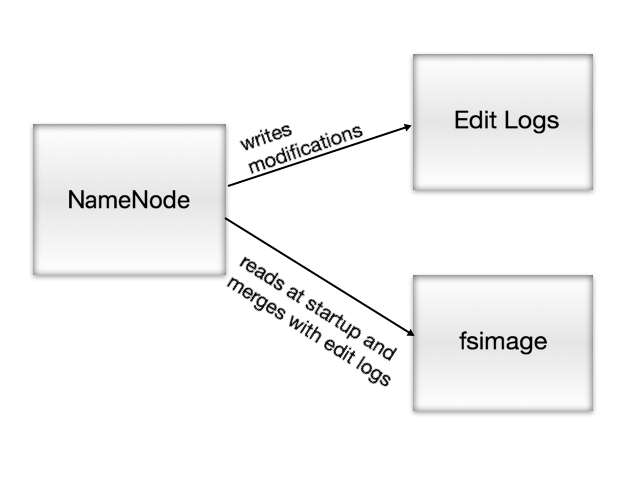
\includegraphics[width=80mm, keepaspectratio]{figures/namenode_problem.png}
	\centering
	\caption{Problem with NameNode}
\end{figure}
The image shows how NameNode stores information \cite{Secondary-NameNode}. There are two different files:
\begin{itemize}
	\item edit logs: the changes made to the file system after the NameNode started
	\item fsimage: a snapshot of the file system when the NameNode started
\end{itemize}
In production clusters, the NameNode restarts are very rare. That means edit logs can grow large and in case of a crash we will lose a huge amount of metadata since the fsimage is very old.

The Secondary NameNode helps to solve this issue. It is responsible for merging the edit logs with fsimage. It collects edit logs on a regular basis and applies them to the fsimage. NameNode will use this fsimage in case of a crash and it can also be used to reduce the startup time of the NameNode.
It is important to remember that the Secondary NameNode is not a real backup NameNode it only merges the edits into the fsimage. 

\begin{figure}[H]
	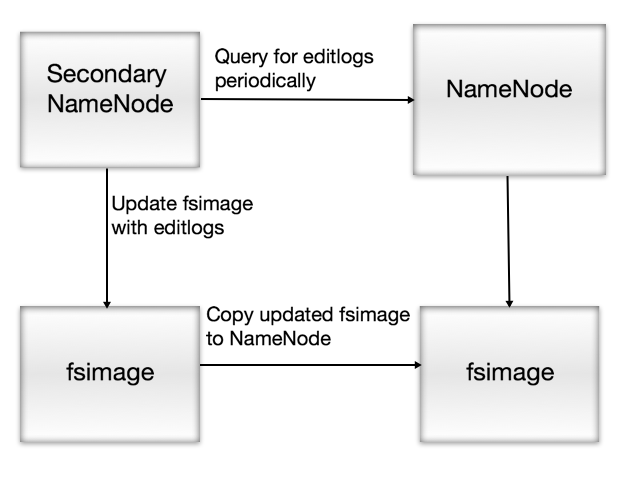
\includegraphics[width=80mm, keepaspectratio]{figures/secondary_namenode.png}
	\centering
	\caption{Solution using the Secondary NameNode}
\end{figure}

\subsection{DataNodes \cite{Shvachko:2010:HDF:1913798.1914427}}
On a DataNode, a block is represented by two files in the native file system. The first contains the data itself, the second is the metadata.

On startup, the DataNodes connect to the NameNode and perform a handshake. This will verify the namespace ID and software version of the DataNodes. If one of them does not match with the NameNode's value, the DataNode automatically shuts down. After a successful handshake, the DataNode registers with the NameNode. DataNode will store it's internal identifier. If restart occurs the DataNodes will be recognizable with the ID, even if they get a different IP address or port. After the ID is registered to the NameNode the will never change. 

 When a DataNode is registered it sends a block report immediately. It contains block id, generation stamp and the length of each block the DataNode hosts. To provide up-to-date information to the NameNode reports are sent every hour. 

DataNodes send heartbeats to the NameNode. It ensures the NameNode that the DataNode is operating and block replicas of the server are available. If the NameNode does not receive a heartbeat from a DataNode it will consider the node to be out of service. The default heartbeat interval is three seconds.

\subsection{HDFS Client \cite{Shvachko:2010:HDF:1913798.1914427}}
User applications can access the file system using the HDFS client which exports the HDFS file system interface. HDFS supports operations similar to a traditional file system: read, write, create or delete files and create or delete directories. The user can refer to files or directories using paths in the namespace.

When someone reads a file, HDFS Client asks the NameNode for the list of DataNodes that host replicas of the blocks of the file. Then it will directly contact the DataNode and request the desired block.

\begin{figure}[H]
	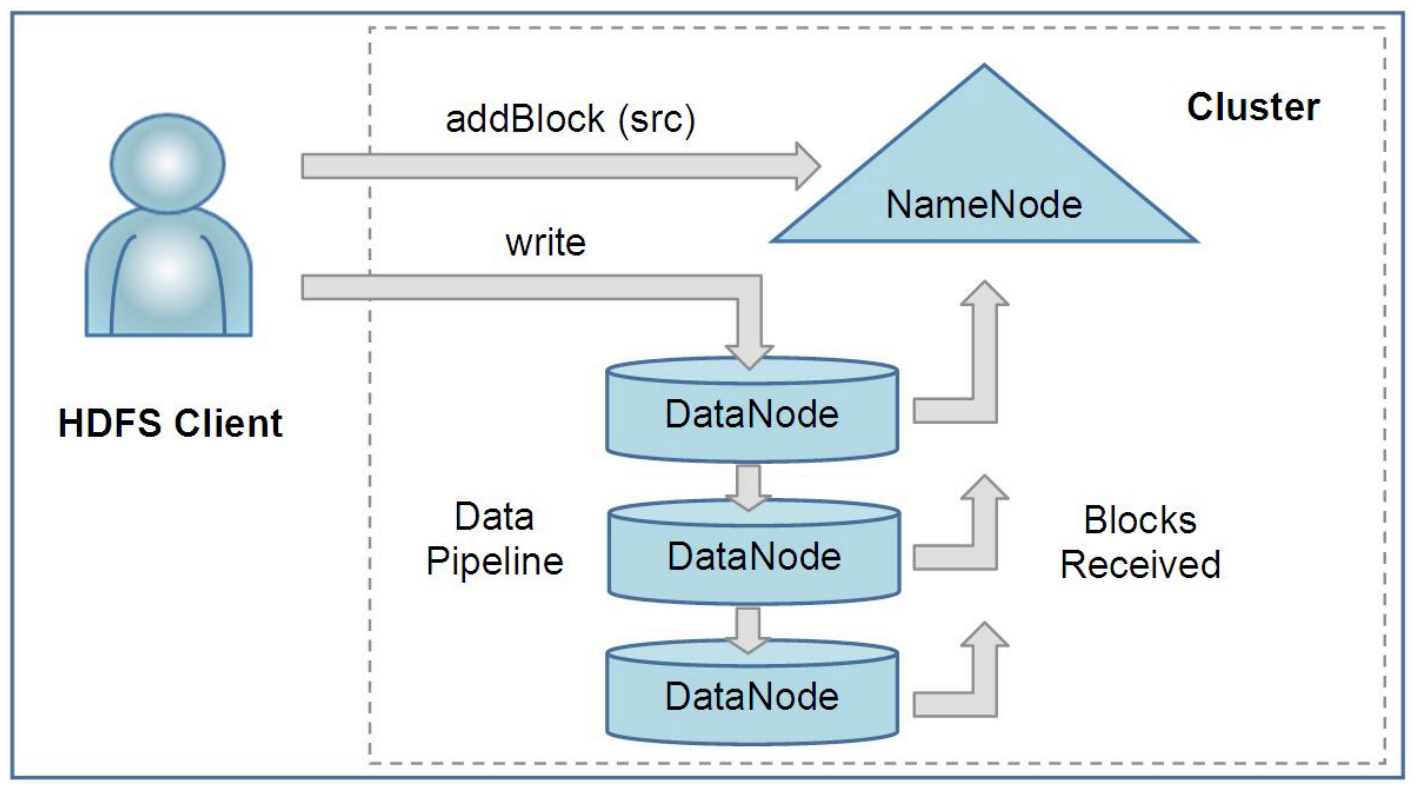
\includegraphics[width=100mm, keepaspectratio]{figures/hdfs_client.png}
	\centering
	\caption{HDFS file writing}
\end{figure}
The client creates a new file by giving its path to the NameNode. For each block, the NameNode will return a list of DataNodes to place the replicas. The client pipelines data to the given DataNodes, and they will confirm the creation of the block to the NameNode.

\section{MapReduce}
MapReduce is a programming model for processing data sets. Users specify two functions \cite{Dean:2004:MSD:1251254.1251264}:
\begin{itemize}
	\item map function: processes a key-value pair to generate a set of key-value pairs
	\item reduce function: merges the intermediate values associated with the same key
\end{itemize}

Programs written in MapReduce are automatically executed parallelly on large clusters. Using this, programmers with no experience in parallel programming and distributed systems can utilize the available resources on the cluster.
\paragraph{Example \cite{MapReduce-example}}
This example shows how MapReduce handles the problem of counting words. Let's say, we have the following list of words: 
\begin{center}
	\textbf{Dear, Bear, River, Car, Car, River, Deer, Car, Bear}
\end{center}

\begin{figure}[H]
	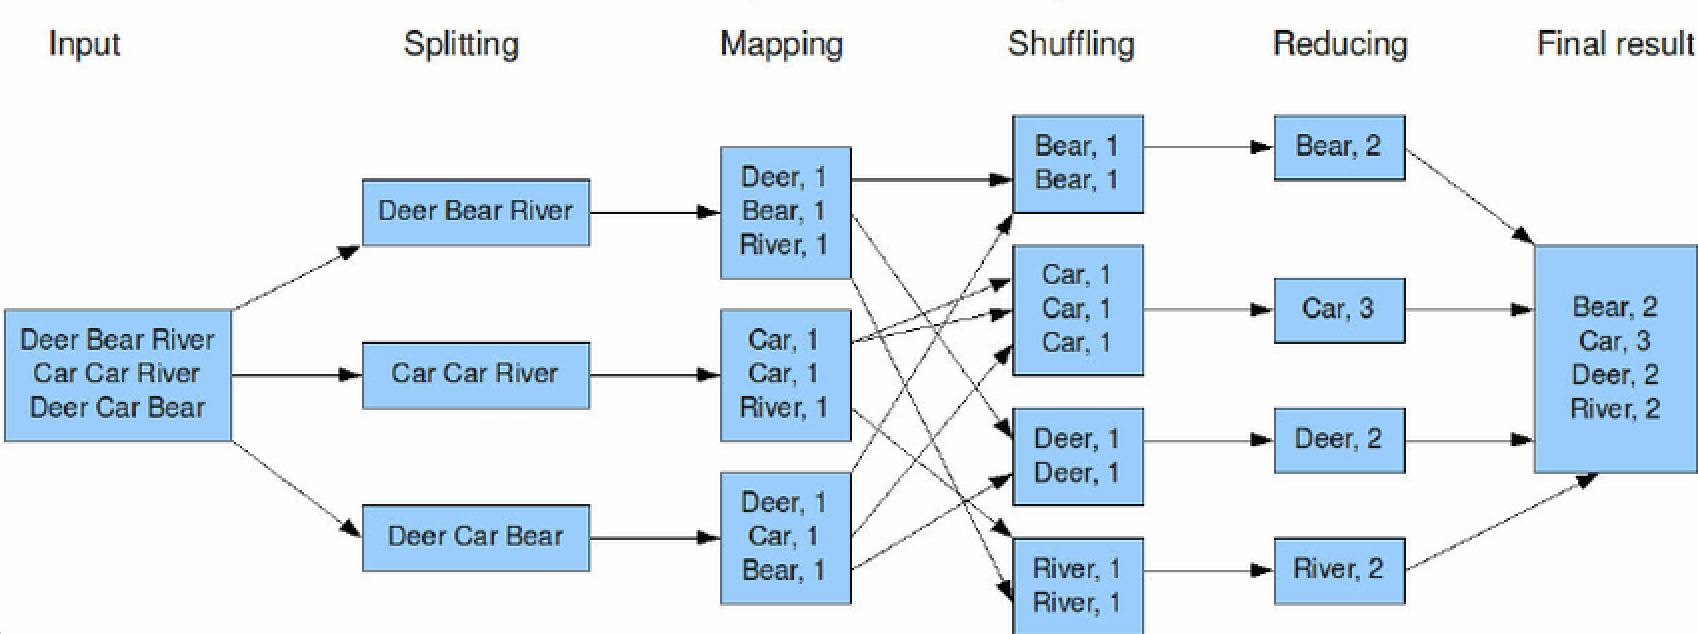
\includegraphics[width=150mm, keepaspectratio]{figures/MapReduce_Example.png}
	\caption{The MapReduce word count process \cite{MapReduce-example-figure}}
	\centering
\end{figure}
\begin{itemize}
	\item \textbf{Splitting}: the first step is dividing the input into splits. This will distribute the work among the Map nodes.
	\item \textbf{Mapping}: tokenize the words in each mapper and giving a value of 1 for each word, since every word in itself will occur once.
	\item \textbf{Shuffling}: partition takes place with shuffling and sorting: this way pairs with the same key will be sent to the same reducer.
	\item \textbf{Reducing}: a reducer gets the list of pairs and counts the number of ones in this list.
\end{itemize}

\subsection{Advantages of MapReduce \cite{MapReduce-example}}
\subsubsection{Parallel processing}
In MapReduce we divide the job among multiple nodes, so they can work on their part of the data parallelly. This way the data processing is done by multiple machines instead of one, so the time is significantly reduced.
\subsubsection{Data locality}
In Hadoop MapReduce, instead of moving data into the processing unit, we move the processing unit to the data. The traditional approach has its limit when it comes to processing big data. Moving huge data is costly: network issues can occur and the master node (where data is stored) can get overloaded and may fail. 

However, the MapReduce approach is very cost efficient, since all the nodes are working simultaneously on their part of the data and there is no chance of a node getting overloaded.

Using Hadoop we just need to provide the map and reduce functions, the rest is done by the framework.  The word count example would look like the following in Java:
\subsubsection{Map}
\begin{lstlisting}[language=Java]
	public void map(LongWritable key, Text value, Context context) throws IOException,InterruptedException {
		String line = value.toString();
		StringTokenizer tokenizer = new StringTokenizer(line);
		while (tokenizer.hasMoreTokens()) {
			value.set(tokenizer.nextToken());
			context.write(value, new IntWritable(1));
		}
	}
\end{lstlisting}
The input and output of the Mapper is a key/value pair. 

\noindent Input:
\begin{itemize}
	\item Key: the offset of each line
	\item Value: each line
\end{itemize}

\noindent Output:
\begin{itemize}
	\item Key: the tokenized words
	\item Value: the hardcoded value 1
\end{itemize}

\subsubsection{Reduce}
\begin{lstlisting}
	public void reduce(Text key, Iterable<IntWritable> values,Context context) throws IOException,InterruptedException {
		int sum=0;
		for(IntWritable x: values) {
			sum+=x.get();
		}
		context.write(key, new IntWritable(sum));
	}
\end{lstlisting}
Both the input and output of the Reducer is a key/value pair. 

\noindent Input:
\begin{itemize}
	\item Key: unique words, generated after the sorting and shuffling phase
	\item Value: a list of integers corresponding to each keys
	\item \eg Bear, [1, 1]
\end{itemize}

\noindent Output:
\begin{itemize}
	\item Key: all the unique words in the input text file
	\item Value: number of occurrences for each unique word
	\item \eg  Bear, 2; Car, 3
\end{itemize}

The traditional way to execute MapReduce operations is that the users specify the Map and Reduce functions in Java. However, this approach has some problems:
\begin{itemize}
	\item it is not a high-level language for data processing
	\item data scientists do not understand Java. They came from the world of traditional databases, where SQL is used.
	\item even a simple problem (like word counting) resulted in hundreds of lines of code.
\end{itemize}

Although, the Hadoop MapReduce framework is written in Java, with the help of Streaming API we can create Map and Reduce functions in any languages.

MapReduce gives us a solution for many big data problems. However, for some scenarios, MapReduce is not the ideal choice: \eg real-time analysis. In Hadoop 1.0 we could not use components other than MapReduce (for example Apache Storm which is ideal for real-time computation). The desire for utilizing the potential provided by the distributed file system (HDFS) in other solutions has grown. YARN provides a solution to fulfill this claim.

\section{Yarn \cite{YARN}}
\subsection{Hadoop 1.0 resource management}
Previous to Hadoop 2.0, a single JobTracker had the responsibility to monitor the resources and distribute the MapReduce jobs for the DataNodes and monitor these jobs. 

In Hadoop 1.0 the MapReduce module was responsible for cluster resource management and data processing as well.

\begin{figure}[H]
	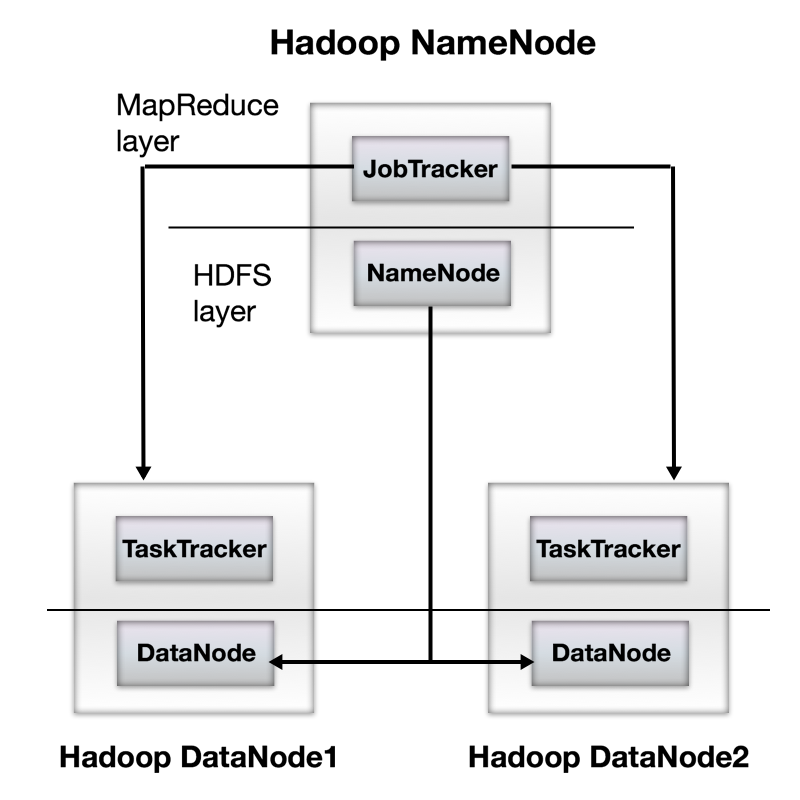
\includegraphics[width=100mm, keepaspectratio]{figures/hadoop10.png}
	\centering
	\caption{Hadoop 1.0 architecture\cite{Hadoop1.0-problems}}
	\centering
\end{figure}

\noindent Resource management in Hadoop 1.0 \cite{Hadoop1.0}:

Clients submit jobs to the JobTracker which turns to the NameNode. It returns the location of the data. The JobTracker locates TaskTracker nodes with available slots close to the data and sends the job to the chosen TaskTracker nodes. After the job has started the JobTracker monitors the chosen TaskTracker nodes. If they do not send heartbeats frequently, they are deemed to have failed so the task will be scheduled on a different TaskTracker. The JobTracker gets a notification if a task fails. It decides what to do then: it may send the job to another TaskTracker, it can mark the record as something to avoid, or it may even put the TaskTracker to blacklist since it is unreliable. If the JobTracker sees that the task is finished, it will update its status. Clients poll the JobTracker for information.

The architecture of Hadoop 1.0 has many problems \cite{Hadoop1.0-problems}:
\begin{itemize}
	\item  It \textbf{limits scalability} since the JobTracker runs on a single machine doing multiple tasks it becomes a bottleneck: resource management, job and task scheduling, monitoring are done by the JobTracker.
	\item JobTracker is a \textbf{Single Point of Failure}. If it goes down, all the jobs are halted.
	\item In Hadoop 1.0 \textbf{JobTracker is tightly integrated with the MapReduce} module so only MapReduce applications can run on Hadoop. Although MapReduce is powerful enough to express many data analysis algorithms (mostly batch-driven data analysis), it is not always the optimal paradigm. It is often desirable to run other computation paradigms on Hadoop like real-time analysis and Message-Passing approach, \etc. Since HDFS makes it easy to store large amounts of data it is desirable to utilize this for other big data problems.
\end{itemize}

Developers recognized that splitting the responsibility to resource management and application monitoring has serious benefits. YARN is a re-architecture of Hadoop that allows multiple applications to run on the same platform. With YARN, applications run "in" Hadoop, instead of "on" Hadoop. This takes Hadoop beyond a batch processing application to a "data operating system" where HDFS is the file system and YARN is the operating system. 

\begin{figure}[H]
	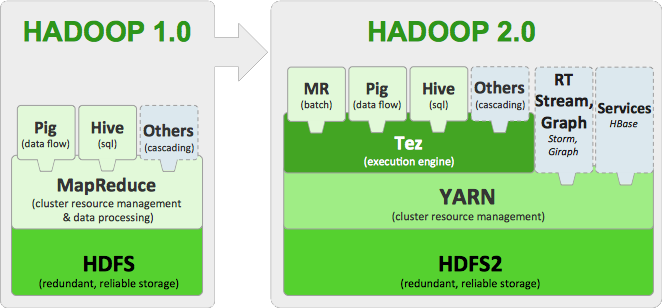
\includegraphics[width=100mm, keepaspectratio]{figures/hadoop10vs20.png}
	\centering
	\caption{From Hadoop 1.0 to Hadoop 2.0}
	\centering
\end{figure}

The fundamental idea behind YARN is to split up the functionalities of resource management and job scheduling/monitoring. In YARN we have a global ResourceManager (RM) and ApplicationMaster (AM) for each application.

\textbf{ResourceManager} is responsible for distributing the resources among all the applications in the system. The \textbf{NodeManager} is a per-machine agent who monitors the resource usages (CPU, memory, network, disk) of the containers and reports them to the ResourceManager. 

The \textbf{ApplicationMaster} is framework specific, and its task is to ask the ResourceManager for resources when needed. It is also working with the NodeManager to execute and monitor tasks.

The ResourceManager is divided into two main components: Scheduler and ApplicationsManager.
\begin{itemize}
	\item The Scheduler is responsible for allocating resources to applications running in the cluster. It schedules based on the resource requirements of each application. The Scheduler does not perform monitoring or status tracking.
	\item The ApplicationsManager accepts job-submissions. It negotiates the first container for executing the application specific ApplicationMaster. It is also responsible for restarting the ApplicationMaster if it fails. 
\end{itemize}

\begin{figure}[H]
	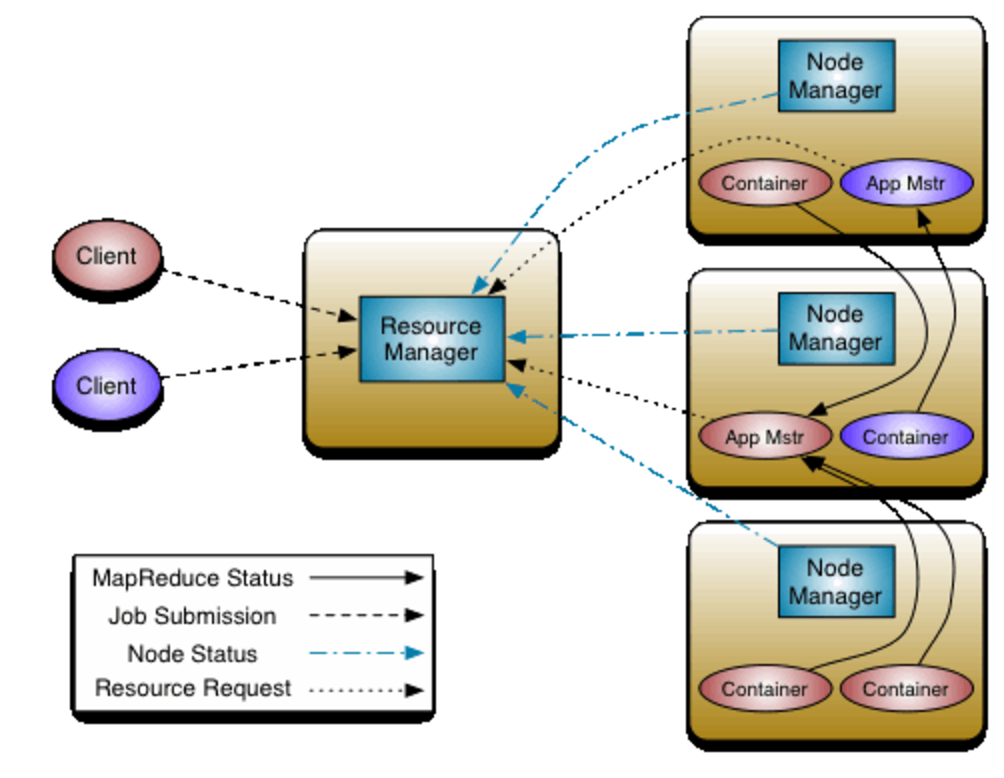
\includegraphics[width=110mm, keepaspectratio]{figures/yarn.png}
	\centering
	\caption{Yarn architecture}
	\centering
\end{figure}

In summary, with YARN Hadoop is able to run applications that do not follow the MapReduce model since it decouples the resource management and scheduling capabilities of MapReduce. With the help of YARN, we can efficiently utilize the resources and can run multiple applications in Hadoop, all sharing a common resources.
\chapter{Apache Hive}
Hadoop is a popular implementation of the map-reduce model and used widely to process and store extremely large datasets. However, a map-reduce program is very low level and difficult to maintain or reuse. Data scientist come from a world, where SQL is the standard of data processing. Apache Hive gives us a data warehouse solution built on top of Hadoop to write SQL-like queries so we can utilize the advantage of a declarative language. The language similar to SQL is called HiveQL.

\section{Hive \vs RDBMS}
This section shows the main differences between Hive and traditional databases (\eg MySQL, Oracle, MS SQL \etc).

Hive supports SQL interface but it is not a full database. It follows WORM (Write Once Read Many) model while RDBMS is designed for Write and Read many times. Hive uses schema on read and traditional databases offer schema on write. Looking into Hive's approach, data is not validated until it is read. We can define multiple schemas to the same data and it provides a fast initial loading since the operation is just a copy and write. However, the schema on read approach has some drawbacks. Schema check on write ensures that the data is not corrupt and it provides a better query performance: when we read data, schema checking is not needed. Hive is a better choice when the schema is not available at loading time since it can be added later dynamically. 

From Hive 0.13, Hive supports transactions \cite{Hive-apache} and full ACID semantics at row level, but with many limitations. Previous to this, atomicity, consistency and durability were available and only at partition level. With introducing transactions Insert, Update and Delete keywords were added to HiveQL. 

The maximum data size allowed in a traditional RDBMS is 10's of Terabytes. However, Hive can easily handle Petabytes.

\subsection{Conclusion}
Hive is a great choice if we want to analyze large, relatively static data sets, fast querying is not necessary and easy, low-cost scalability is required. RDBMS provides fast responses for analyzing data dynamically, but scalability and maximum data size are limited.

\section{Data storage}
Hive structure data in the following units  \cite{Hive-paper, Hive-apache}:
\begin{itemize}
\item \textbf{Databases}: namespaces to avoid conflicts of table, partition or bucket names.
\item \textbf{Tables}: storage unit for data with the same schema. Tables maps to directories in HDFS.
\item \textbf{Partitions}: Tables can have many partition keys. These will determine how data is stored. In HDFS partitions map to subdirectories in the table's directory. This way we can speed up the analysis. Instead of running the query in the whole table, Hive will only run our query in the relevant partitions (see example below). Partition columns are virtual, which means they are not part of the data itself.
\item \textbf{Buckets}: Data can be divided into buckets based on the hash value of a column. These are helpful for efficiently sample data. Buckets are stored in files in the table's or partition's directory.
\end{itemize}

\subsection{Example}
This example shows how Hive data units map to HDFS and and how partitioning tables can speed up queries.

Hive tables map to \texttt{<warehouse\_root\_directory>/table\_name} directory. As default, the warehouse root directory is /user/hive/warehouse. This can be changed with the corresponding hive configuration value.
\begin{lstlisting}
	CREATE TABLE test_table(c1 string, c2 int) 
		PARTITIONED BY (date string, hour int);
\end{lstlisting}

The above SQL statement will create a table with two columns and two partitions and it will be stored in  \texttt{/user/hive/warehouse/test\_table} directory in HDFS. For every distinct date and hour value, a partititon will exists. Although, the partition columns are not part of the data, they are stored in the table metadata. 

New partitions can be added either with the INSERT or the ALTER statement. These commands will create the corresponding HDFS directories: 

\texttt{/user/hive/warehouse/test\_table/date=2018-01-01/hour=12 and /user/hive/warehouse/test\_table/date=2018-01-02/hour=11}.

\begin{lstlisting}
	INSERT OVERWRITE TABLE
		test_table PARTITION(date='2018-01-01', hour=12)
	SELECT * FROM t;
	
	ALTER TABLE test_table
		ADD PARTITION(date='2018-01-02', hour=11);
\end{lstlisting}

Hive can use these information for pruning the directories to be scanned for query execution. 
\begin{lstlisting}
	SELECT * FROM test_table WHERE date='2018-01-01';
\end{lstlisting}
In case of this query, Hive will only scan the files in \texttt{/user/hive/warehouse/test\_table/date=2018-01-01} directory. Partitioning our data has significant impact on the time taken by queries.

Although, data in Hive is always in the corresponding directory (\texttt{<warehouse\_root\_directory>/table\_name}), Hive is able to query data stored in other locations in HDFS. In order to do this, we can create EXTERNAL tables as the following statement shows:
\begin{lstlisting}
	CREATE EXTERNAL TABLE test_external(c1 string, c2 int)
		LOCATION '/user/example_table/example_data';
\end{lstlisting}

Hive assumes that the external table in its internal format. The difference between an external and normal (managed by Hive) table is that the drop table command doesn't effect the data itself on an external table. However, on a normal table, it drops the associated data.

\section{Architecture}
The main components of Hive are the following \cite{Hive-paper}:
\begin{itemize}
	\item \textbf{Driver}: manages the lifecycle of a HiveQL query by creating a session for it. The driver also collects the result after the execution phase.
	\item  \textbf{MetaStore}: stores metadata about tables, columns or partitions. For example, it stores the table schema and location.
	\item \textbf{Compiler}: compiles the HiveQL statement and generates the execution plan using the partition and table metadata obtained from the MetaStore. First, it parses the query and does semantic analysis. Then converts it into AST (Abstract Syntax Tree) and after compatibility checking to a DAG of Map and Reduce tasks (if Hadoop MapReduce is the execution engine). 
	\item \textbf{Optimizer}: transformations are done to get an optimized DAG for better performance. It is an evolving component. In the earlier stage, only rule-based optimization was available which performed column pruning and predicate pushdown. Later, map-side join was introduced and several other join optimization, also cost-based optimization was added.
	\item \textbf{Execution Engine}: executes the plan created by the compiler. The plan is a DAG of stages. The engine manages the dependencies between these stages and executes them in the corresponding component. Hive is compatible with 3 execution engines: MapReduce, Apache TEZ and Spark which can run in Hadoop YARN.
	\item \textbf{HiveServer2}: a service that provides a thrift interface so clients can execute queries against Hive. Thrift is an RPC (Remote Call Procedure) framework for defining services for multiple languages.
	\item \textbf{Clients}: multiple clients are available to interact with Hive. Beeline (CLI), JDBC/ODBC, Python or Ruby client \etc.
\end{itemize}

\begin{figure}[H]
	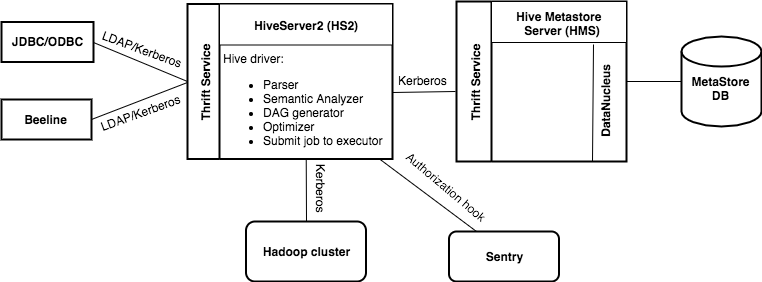
\includegraphics[width=150mm, keepaspectratio]{figures/Hive_architecture.png}
	\centering
	\caption{Hive architecture}
\end{figure}

Clients can connect to  using its Thrift Service. HS2 supports authentication of the clients using Kerberos or LDAP authentication. Hive Metastore server also supports Kerberos authentication for Thrift clients.

Sentry is a role-based authorization module for Hadoop, so we can control the priviliges for authenticated users. Hive can use Sentry over an "authorization hook", which Sentry registers to Hive configuration file if secure cluster is enabled. 

HMS uses DataNucleus to persist metadata, so any relational database supported by it cal be used: it can be either embedded (\eg Derby) or remote (\eg MySQL) Metastore database.

\section{Life of a Query}
\begin{figure}[H]
	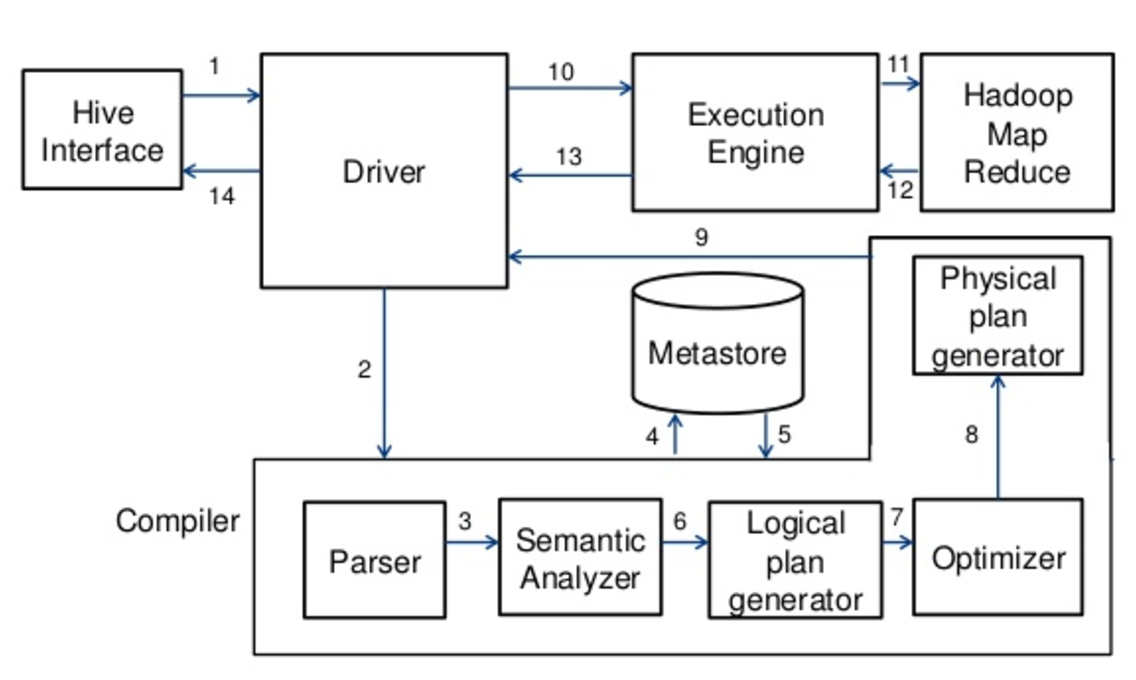
\includegraphics[width=150mm, keepaspectratio]{figures/hive-query.png}
	\centering
	\caption{Life of a query  \cite{Hive-query-figure}}
\end{figure}
User submits a query using one of the available Hive clients. HiveServer2 recieves the query through its Thrift interface (1). Compilation takes place: 

First, it parses the query (2), so the query string is transformed into a parse tree using the open source Apache ANTLR.  The semantic analyzer (3) converts the parse tree into a block-based query representation (Query Block Tree). At this phase connection to Metastore is made (4, 5) to gather information about the tables used by the query, like partition information for later pruning. It checks type compatibility and flag semantic errors. 

The logical plan generator (6) transforms the internal representation to an operator tree, which is the logical plan. These operators can either be relational algebra operators (like filter, join) or Hive specific operators (\eg reduceSink) which are used to convert the query later to a series of MapReduce jobs.

Optimization takes place for better performance (7). Most common optimizations are: 
\begin{itemize}
	\item Column pruning, so only columns needed by the query are kept
	\item Predicate pushdown: this way the rows can be filtered as soon as possible
	\item Partition pruning: prunes partitions that do not satisfy the predicate
	\item Map-side join: if joining two tables and one of them is small, map-side join can be done. This way the small table will be copied to the memory all the Map nodes.
	\item \etc
\end{itemize}

At physical plan generation (8) the logical plan is split into a series of Map, Reduce and HDFS tasks (of course if the execution engine is Spark, then to Spark tasks). 

The Driver gets back the physical plan (9) and sends (10, 11) it to the corresponding execution engine (which is MapReduce by default). In this case, Hadoop executes the series of Map and Reduce tasks an returns the result to the Driver (12, 13), which sends it to the user (14).

\section{Hive memory limitations}
HiveServer2 and Hive Metastore require massive resources, especially memory wise. If we want to run up to 40 concurrent queries the recommended heap size range is 12-16 GB. Once we go above 16 GB it is recommended to split HS2 into multiple instances and load-balance them \cite{Hive-memory-problems}.

Although, with correct configuration and setup we can make our HiveServer2 instance long living, crashes can occur because of Out Of Memory error (OOM) in certain use-cases. Thus, minimizing the memory footprint whenever we can is a must.

\noindent The memory reserved by HiveServer2 can grow significantly in these situations  \cite{Hive-memory-problems}: 
\begin{itemize}
	\item When we have many table partitions, HS2 needs to load all the partition metadata from HMS. This can cause a real memory issue, and  HiveServer can run out of heap memory and can crash.
	\item Concurrent connections can be made to HS2, and memory is directly proportional to the number of connections. 
	\item Complex queries that access a large number of partitions from multiple tables can easily crash HS2.
\end{itemize}

If any of these conditions exists, Hive can slow down, refuse further connections, queries can fail and long query execution can occur. If the Garbage Collector cannot handle the memory reserved, HiveServer2 can go OOM.

\chapter{Memory Analysis}
To get a better insight on how Hive uses memory, I needed to build a basic model when and why Hive's reserved memory grows. During my work, I mainly focused on HiveServer2. The first step toward the model building was to get basic knowledge about Hive's code base and the query compilation process. The query life cycle mentioned in the previous chapter helped, but I had to find those steps in the code. If I have these points I am able to start measuring and maybe find some memory wastes.

\section{Finding the measuring points}
Hive has around 2 million lines of code so locating the main steps of the query processing was challenging. 

As a starting, the user enters a query in the client. At this point, I run Hive locally, so the simplest way for submitting queries against Hive was using Beeline command line client. HS2 gets the query through its Thrift interface. After this, the query goes to the \textit{Driver} class, which is the main class for compiling and executing queries.

The Driver has two methods that are important for me: \textit{run} and \textit{runInternal}. The \textit{run} method gets called first, which basically just delegates to the \textit{runInternal} method. These two functions return with a \textit{CommandProcessorResponse}, once the compilation and execution are done. 

\noindent The runInternal does the two main steps:
\begin{itemize}
	\item \textit{Driver.compile}: gets the command string and parses, analyses the query and generates the execution plan.
	\item \textit{Driver.execute}: gets the execution plan and executes it on a specific engine (MapReduce, Spark or TEZ).
\end{itemize}

\subsection{Compile}
The first step of the compilation is the parsing. It takes a string and returns an Abstract Syntax Tree (AST or the Parse Tree).

\begin{lstlisting}
public int compile(String command, ...) {
...
	ASTNode tree;
	try {
		tree = ParseUtils.parse(command, ctx);
	} catch (ParseException e) {
...
}
\end{lstlisting}
\subsubsection{Semantic Analyzis}
After the AST is generated, the compile process will continue with the semantic analyzer. The type of the analyzer will depend on the query type we are running. For SELECT and INSERT the \textit{SemanticAnalyzer} class is used. 

\begin{lstlisting}
public int compile(String command, ...) {
...
	BaseSemanticAnalyzer sem = SemanticAnalyzerFactory.get(queryState, tree);
...
	sem.analyze(tree, ctx);
...
}
\end{lstlisting}

The SemanticAnalyzer class is the main phase during compilation. It checks for semantic errors, fetches metadata from Metastore, generates and optimizes the query plan. The \textit{analyze} method of the \textit{BaseSemanticAnalyzer} is called from the Driver's \textit{compile} method, and it delegates the call to the corresponding analyzer. From now on, I will write about the \textit{SemanticAnalyzer} class and its phases (which is executed for SELECTS and INSERTS).

\begin{lstlisting}
void analyzeInternal(ASTNode ast, PlannerContext plannerCtx) {
	//(1)
	if (!genResolvedParseTree(ast, plannerCtx)) {
		return;
	}
	//(2)
	Operator sinkOp = genOPTree(ast, plannerCtx);
	...
	//(3)
	...
	resultSchema = convertRowSchemaToViewSchema(...);
	...
	//(4)
	Optimizer optm = new Optimizer();
	... = optm.optimize();
	...
	//(5)
	TaskCompiler compiler = TaskCompilerFactory.getCompiler(conf, pCtx);
	compiler.compile(pCtx, rootTasks, inputs, outputs);
	...
}
\end{lstlisting}

\begin{enumerate}
	\item Fetches metadata and fills the Parse Tree with it so it becomes a Resolved Parse Tree.
	\item The Operation Tree gets created which will contain operators that process data read from the table. This tree is called by the Map and Reduce methods.
	\item The semantic analyzer will deduce the schema of the result set from the row schema
	\item A logical optimization is done on the Operator Tree. There are two types of optimization: one that transforms the Operator Tree (like removing unnecessary operations) and one that does not (predicate pushdown, vectorization \etc).
	\item Physical optimization and translation to the target execution engine take place. The output of this stage is the query plan. It can optimize the tree according to the engine used. For example in MR, common join can be translated to map-side join, if one of the tables is small enough to fit into the memory of the map nodes.
\end{enumerate}

\begin{lstlisting}
public int compile(String command, ...) {
	...
	sem.validate();
	...
}
\end{lstlisting}

After the semantic analysis is completed, the Driver will validate the plan. When it completes, the compilation ends and Hive will continue with the execution.

\clearpage
\section{Measure the memory of HiveServer2}
If I want to measure the memory usage of Hive, I need a something to create and analyze heap dumps and generate memory statistics. There are several tools to choose from. In this section, I will present the tools I considered and the method I used to get a better understanding of HS2 memory patterns.

\subsection{Tools for generating heap dumps and statistics}
For creating heap dumps and statistics of the memory, I decided to use a command line tool. In contrast of a UI tool, it has the benefits to generate heap dumps and statistics automatically. 

\subsubsection{jmap}
\textit{jmap} \cite{jmap-jcmd} can be used to obtain heap dumps and histograms from a running java process.

To gather information about a running Java program we need its process ID (PID). Using this we can easily create the heap dump with the \textit{-dump} option. If we do not want to analyze large heap dumps, just to get the objects that reserve the most memory, we can use the \textit{-histo} option. It will print a histogram of the heap, containing each Java class, the number of objects and memory sizes per class.

\subsubsection{jcmd}
\textit{jmap} would have been a perfect choice for measuring memory. However, it is recommended to use the latest utility, which is called \textit{jcmd} \cite{jmap-jcmd}. It has enhanced diagnostics capability and its perfomance overhead is reduced. 

The usage of jcmd is similar to jmap. For creating heap dumps we can use \textit{jcmd <PID> GC.heap\_dump}. If we want to obtain class histogram we can do that with the \textit{jcmd <PID> GC.class\_histogram} command. With the \textit{jcmd <PID> GC.heap\_info} command we can gather basic information of the heap: \eg young and old memory of the process.

I decided to use jcmd in my future work to gather memory information automatically and generate heap dumps at the measuring points identified in the previous section.

\subsection{Tools for analysing heap dumps}
Creating heap dumps with a CLI tool is easier, however analysing those requires a tool with user interface. 

\subsubsection{YourKit}
\textit{YourKit} provides great analysing capabilities for heap dumps. We can use it for profiling local or remote Java applications. It has controllable overhead. Although, it is a great tool for profiling Java applications, it is a commercial software and only has 15 days of free licence.

\subsubsection{VisualVM}
\textit{VisualVM} provides a great visual interface for profiling Java applications and browsing heap dumps. It offers multiple views for analysing them. We can get the summary of the dump which contains the total bytes, classes and objects. 

With the "classes view" we can get information about the reserved memory and number of instances for each class. We can calculate the retained memory, which is the memory that would be freed if the objects would be garbage collected.

\subsubsection{JXRay}
JXRay \cite{jxray} is a memory analysis tool for Java applications. It creates an HTML report of a given heap dump. It can automatically detect common problems, like data duplication or non-optimal use of data structures. 

JXRay can give us a compact report, even if the heap dump analyzed is 10's of GB. It can calculate how much memory taken by a collection's internal representation and their workload since JXRay knows about the internal representation of common java collections (HashMap, ArrayList \etc).

\begin{figure}[H]
	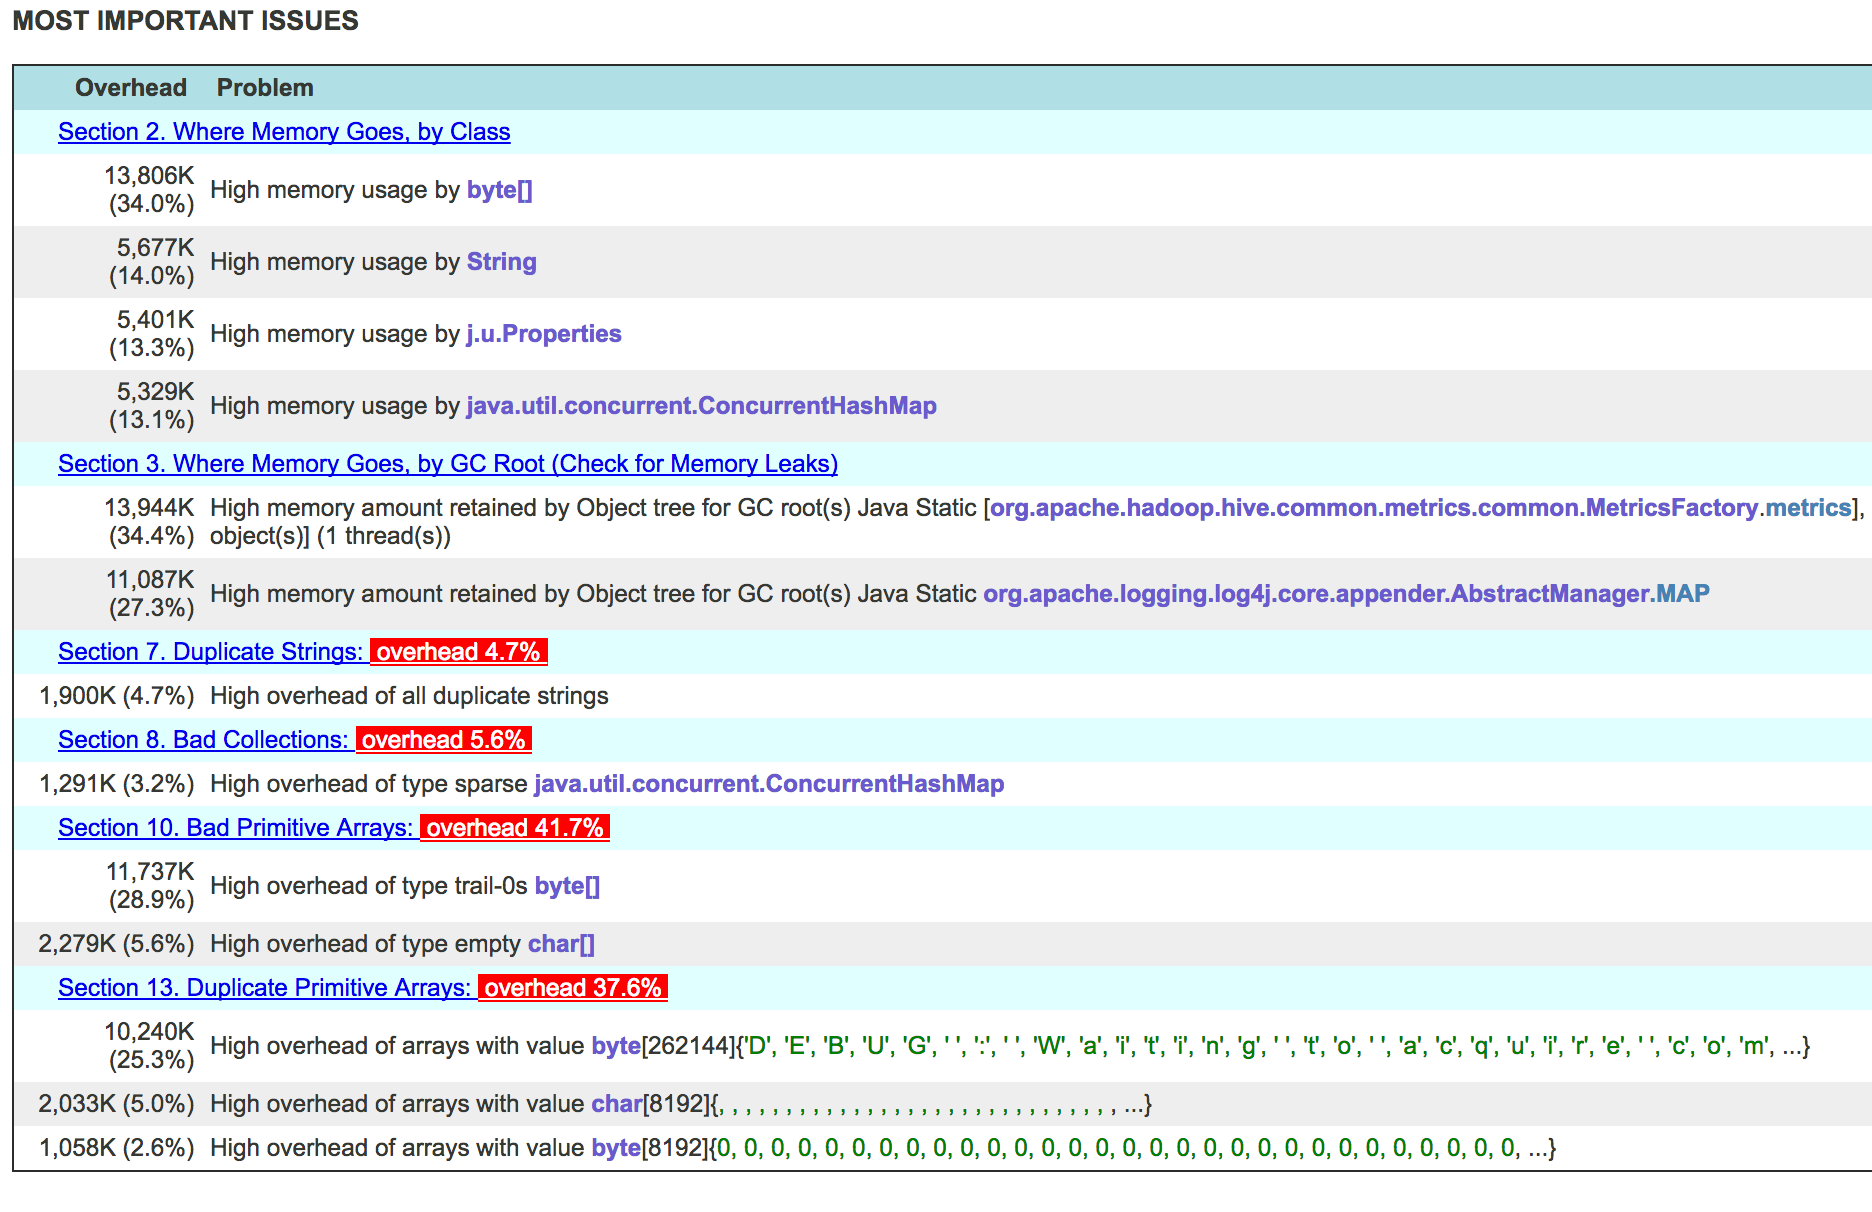
\includegraphics[width=150mm, keepaspectratio]{figures/jxray_sample.png}
	\centering
	\caption{Sample JXRay report summary}
\end{figure}

\subsubsection{The selected tool}
I decided to use VisualVM for visual memory analysis since it has great capabilities for summarizing the most important information about a heap dump and with its help, I am able to walk through the memory tree easily.

During my work, I also used JXRay, since it can automatically detect the most common memory problems and give me an overview of the possible issues a Java application has.

\clearpage
\subsection{Creating the code to measure memory}
With the available tools, I am able to generate heap dumps really easily. However, to get a model how Hive uses the memory, I should gather statistics and heap dumps at certain points of the query execution. Clearly, it is not possible by hand. Thus, I needed to create a class in Hive's codebase and integrate the sampling in the identified points found in the previous section.

In order to use jcmd from Java, I needed a way to execute a terminal command from code. With the \textit{ProcessBuilder} java class I am able to create operating system processes with the given attributes. The \textit{Runtime.exec()} method would do the same, but using this command is discouraged. 

Now that I can run a command line tool from Java, I will need the process ID of HiveServer2. Since Hive uses Java 8, I cannot use the new Process API that Java 9 provides. With the help of the \textit{ManagementFactory} class, we can get the managed bean of the runtime system of the JVM. It will return a class implementing the \textit{RuntimeMXBean} interface. The name of the running JVM contains the ID of the process. With the \textit{RuntimeMXBean.getName()} method, I was able to get the PID of HiveServer2. The method will return a string in a format of \textit{pid@hostname}. Using the split method we can get our application's process ID.

To avoid code duplication I created a method for getting the ProcessBuilder which contains the given command and the PID for HiveServer2 is already set.

\begin{lstlisting}
private ProcessBuilder getProcessBuilder(String subCommand){
	ProcessBuilder builder = new ProcessBuilder();
	//Get own pid
	String pid = ManagementFactory.getRuntimeMXBean().getName().split("@")[0];
	builder.command("sh", "-c", String.format("jcmd %s %s", pid, subCommand));
	return builder;
}
\end{lstlisting}

Using the \textit{getProcessBuilder} function, it is really simple to run a terminal command. For example, getting information about the state of the heap or creating a heap dump will look like this:

\begin{lstlisting}
...
 process =  getProcessBuilder("GC.heap_info").start();
 ...
 getProcessBuilder("GC.heap_dump " + path).start();
\end{lstlisting}

\subsubsection{Parsing result}
I am able to create detailed statistics about the current memory state at certain phases of the query. As a first approach, I decided to just use \textit{GC.heap\_info} to see how memory usage looks like at different stages, not caring how much memory is reserved by each class. However, if we look at the result of the \textit{jcmd <PID> GC.heap\_info}, it will look quite messy, and hides the most important details, especially if we have 15 results for each query. An example of how it looks:

\begin{lstlisting}
21566:
PSYoungGen total 1395200K, used 27419K [0x000000076ab00000, 0x00000007c0000000,
0x00000007c0000000)
eden space 1392640K, 1% used
[0x000000076ab00000,0x000000076c5c6c70,0x00000007bfb00000)
from space 2560K, 0% used [0x00000007bfd80000,0x00000007bfd80000,0x00000007c0000000)
to space 2560K, 0% used [0x00000007bfb00000,0x00000007bfb00000,0x00000007bfd80000)
ParOldGen total 1046528K, used 14704K [0x00000006c0000000, 0x00000006ffe00000,
0x000000076ab00000)
object space 1046528K, 1% used
[0x00000006c0000000,0x00000006c0e5c058,0x00000006ffe00000)
Metaspace used 48314K, capacity 48612K, committed 49280K, reserved 1093632K
class space used 5359K, capacity 5440K, committed 5504K, reserved 1048576K
\end{lstlisting}

I only need certain values: allocated young and old memory, and a total memory which is the sum of the young and old values. I created a function called getResult which will read the result from a given process and return in string format. The returned string will look like above, so parsing is needed if I want to gather the important details.

To do this, I made a function (printResultToCSV) which will parse the given string, and print the results to a csv file in a table like format, where the first line is the query, and the columns are the different stages.

\begin{table}[H]
	\begin{tabular}{|l|l|l|l|l|l|l|l|}
		\hline
		\begin{tabular}[c]{@{}l@{}}select * \\ from \\ people2 \\ limit \\ 10000\end{tabular} & \begin{tabular}[c]{@{}l@{}}Before\\ compile\end{tabular} & \begin{tabular}[c]{@{}l@{}}After \\ parse\end{tabular} & \begin{tabular}[c]{@{}l@{}}Resolve \\ Parse \\ tree\end{tabular} & \begin{tabular}[c]{@{}l@{}}Generate\\ OP tree\end{tabular} & \begin{tabular}[c]{@{}l@{}}Logical \\ opt.\end{tabular} & \begin{tabular}[c]{@{}l@{}}Physical\\ opt.\end{tabular} & Validate \\ \hline
		Young                                                                                 & 10552                                                    & 8679                                                   & 13568                                                            & 13154                                                      & 25681                                                   & 23503                                                   & 27467    \\ \hline
		Old                                                                                   & 12296                                                    & 14499                                                  & 14342                                                            & 51493                                                      & 85316                                                   & 85151                                                   & 85926    \\ \hline
		Sum                                                                                   & 22848                                                    & 23178                                                  & 27910                                                            & 64647                                                      & 110997                                                  & 108654                                                  & 113393   \\ \hline
	\end{tabular}
\centering
\caption{Sample output of the parsing}
\end{table}
\subsection{How HiveServer2 uses memory}
I have the code to measure the memory of Hive and get a general picture of the usage at certain phases. With this, I am able to get a better understanding when and why memory goes high. I would like to get an answer to these questions: How does the number of joins increase the memory? Which type of query generates a lot of memory usage: union, group by? If we increase the number of partitions, how it affects the heap size? In this section, these questions will be answered.

The first step is to create a managed table where I will run my queries in the future. Hive faces memory problems when we have a highly partitioned table. I decided that for the first run, 20 000 partitions will be enough. 

The second step was to create queries which will be submitted to Hive. The first question was how the number of joins affects memory? To answer it, I have created queries with an increasing number of joins included. I used self-joins and only increased the number to three. The pattern was clear for only four measures: a simple select query without join operators, and queries with one, two and three. From the output of my parsed CSV file, I generated the following chart that shows the memory increase.

\begin{figure}[H]
	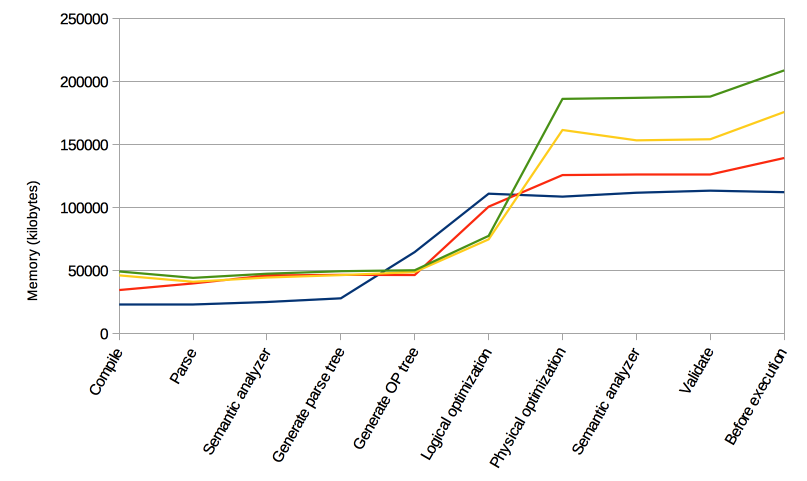
\includegraphics[width=150mm, keepaspectratio]{figures/hs2_joins_memory.png}
	\centering
	\caption{Heap size with increasing number of joins}
\end{figure}

\noindent Queries run with their color in the chart:
\begin{itemize}
	\item select * from tablename (\textcolor{blue}{\rule{2 cm}{2pt} })
	\item select * from tablename t1 join tablename t2 on t1.id=t2.id (\textcolor{orange}{\rule{2 cm}{2pt} })
	\item select * from tablename t1 join tablename t2 on t1.id=t2.id join tablename t3 on t2.id=t3.id (\textcolor{yellow}{\rule{2 cm}{2pt} })
	\item select * from tablename t1 join tablename t2 on t1.id=t2.id join tablename t3 on t2.id=t3.id join tablename t4 on t3.id=t4.id (\textcolor{green}{\rule{2 cm}{2pt} })
\end{itemize}

We can see that the memory change caused by the number of join operators is negligible, only around 20 Megabytes per join. The results were as expected: the memory increased significantly when HiveServer2 connected to the MetaStore and asked for metadata. During physical optimization, Hive loaded metadata to the memory including partition metadata. In a highly partitioned table, this size is notable. Although real queries submitted to Hive by users are much more complicated and contains multiple tables, the model will be quite similar: heap memory will rise when metadata is loaded.

I also wanted to see the memory effects of \textit{group by} and  \textit{union all} operations. I ran 5 more queries including these but did not find anything notable. The pattern remained the same: see the chart below. 

\begin{figure}[H]
	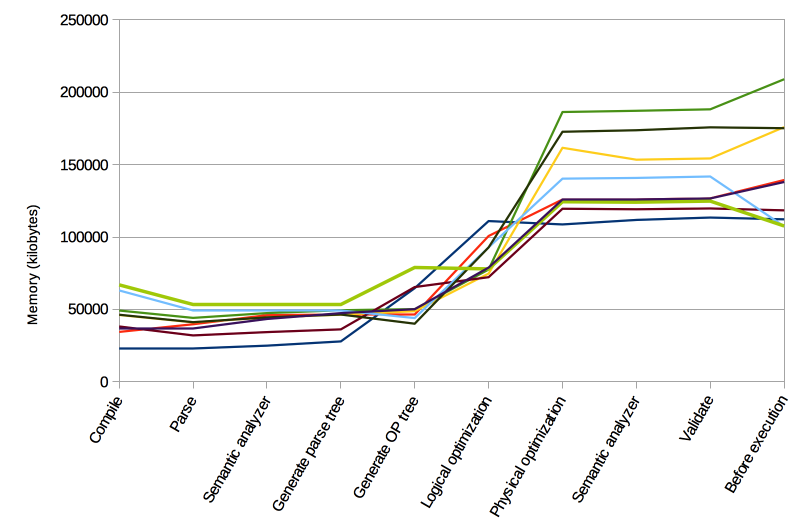
\includegraphics[width=150mm, keepaspectratio]{figures/hs2_memory.png}
	\centering
	\caption{Heap size when running various type of queries}
\end{figure}

I came to the conclusion that for a single connection to HiveServer2, the most important factor that increases heap size is the number of partitions in tables, so I decided to continue my investigation in that area. 

\subsection{Memory consumption of partitions}
A well-known issue in Hive is, if we have a highly partitioned table, the memory goes really high in HiveServer2. As a first step, I wanted to recreate the issue. I created tables with an increasing number of partitions: 200, 2000, 5000, 20000 and 100000 partitions. For each table, I executed the same query which contains a simple select with a self-join. During this, I measured the memory and created a heap dump after the semantic analyzer phase of the compilation. At this stage, the partitions are already loaded so I can analyze how much these objects exactly reserve. To get this information, I analyzed the heap dumps with VisualVM and filtered for the Partition objects. The pattern we can observe was as expected, but I the size of the heap reserved by these objects were smaller than I previously anticipated.

\noindent From the heap dumps I have found that mainly three kind of objects reserve the memory due to partitions, so I will focus on these objects: 
\begin{enumerate}
	\item hive.ql.metadata.Partitions
	\item hive.metastore.api.Partition
	\item hive.ql.plan.PartitionDesc
\end{enumerate}

\begin{table}[H]
	\begin{tabular}{|l|l|l|l|l|}
		\hline
		& \textbf{\begin{tabular}[c]{@{}l@{}}ql.metadata.\\ Partitions\end{tabular}} & \textbf{\begin{tabular}[c]{@{}l@{}}metastore.api.\\ Partition\end{tabular}} & \textbf{\begin{tabular}[c]{@{}l@{}}ql.plan.\\ PartitionDesc\end{tabular}} & \textbf{Sum} \\ \hline
		\textbf{\begin{tabular}[c]{@{}l@{}}200\\ partitions\end{tabular}}     & 300 Kb                                                                     & 288 Kb                                                                      & 108 Kb                                                                    & 696 Kb       \\ \hline
		\textbf{\begin{tabular}[c]{@{}l@{}}2000\\ partitions\end{tabular}}   & 3057 Kb                                                                    & 2946 Kb                                                                     & 1110 Kb                                                                   & 7113 Kb      \\ \hline
		\textbf{\begin{tabular}[c]{@{}l@{}}5000\\ partitions\end{tabular}}    & 7988 Kb                                                                    & 7709 Kb                                                                     & 2793 Kb                                                                   & 18490 Kb     \\ \hline
	\textbf{\begin{tabular}[c]{@{}l@{}}20000\\ partitions\end{tabular}}   & 29999 Kb                                                                   & 28879 Kb                                                                    & 3173 Kb                                                                   & 62051 Kb     \\ \hline
	\textbf{\begin{tabular}[c]{@{}l@{}}100000\\ partitions\end{tabular}} & 165002 Kb                                                                  & 158841 Kb                                                                   & 60531 Kb                                                                  & 384374 Kb    \\ \hline
	\end{tabular}
\centering
\caption{Memory of partitions}
\end{table}

\begin{figure}[H]
	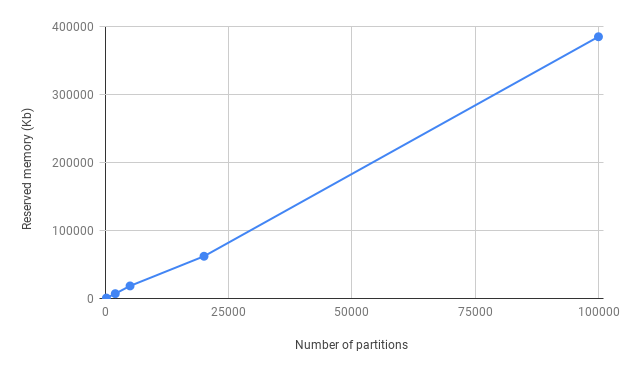
\includegraphics[width=150mm, keepaspectratio]{figures/partitions_chart.png}
	\centering
	\caption{Reserved memory by partitions}
\end{figure}

As we see, for 100.000 partitions the reserved memory is aroung 385 Megabytes. Before taking the samples, I expected higher memory consumption. However, with a little investigation I found that the memory waste around partitions was already somewhat decreased \cite{hive-partitions}. \textit{PartitionDesc} objects has a \textit{java.util.Properties} field. These \textit{Properties} fields in the \textit{PartitionDesc} most often are the same. Interning these saves a big amount of memory. In a later section, I will write more about the interning solution because it gave me an idea to fix another memory related issue.

However the memory reserved by partitions is still high enough, so I decided to take a look at the generated heap dumps and try to find wastes or problems that affects memory.

\subsection{Where does the memory go?}
I analyzed the heap dump generated after the semantic analyzer phase when self-joining a table with 100000 partitions. It showed an interesting fact: 47.1\% (~853 Megabytes) of retained memory is reserved by Strings. Retained means, that if the Garbage Collector frees them, we win that amount of memory. 

\begin{figure}[H]
	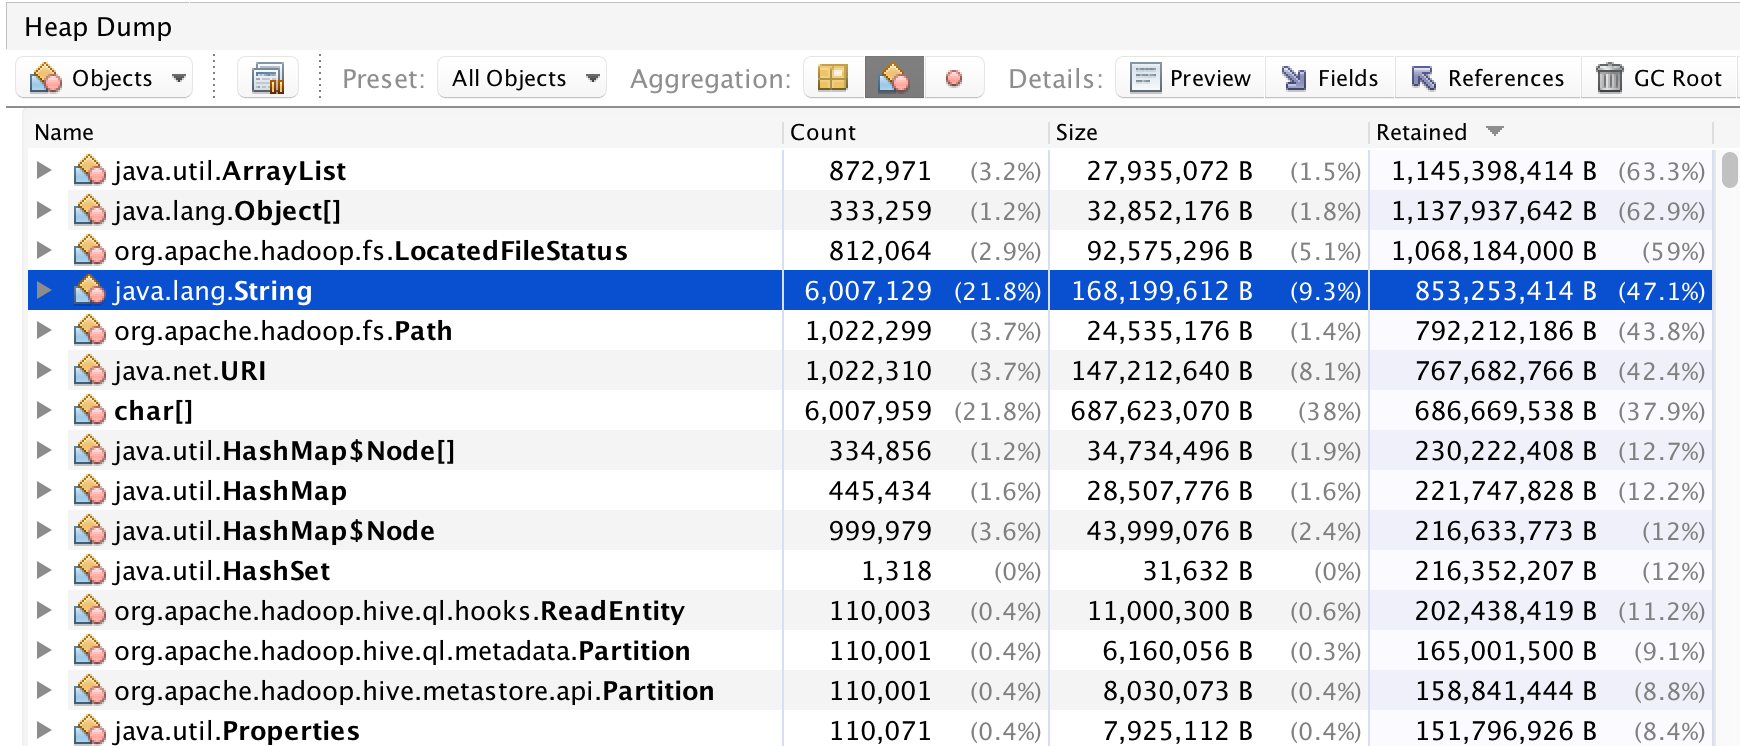
\includegraphics[width=150mm, keepaspectratio]{figures/string_memory.png}
	\centering
	\caption{Memory reserved by Strings}
\end{figure}

We also see in the above image that \textit{hadoop.fs.Path} objects reserve 792 Megabytes. It seems too much considering that we only speak about the location of a file in the filesystem. As a next step, I looked inside the Path objects to see if this is a waste or not.

\subsubsection{Memory waste in HDFS Path}
\begin{figure}[H]
	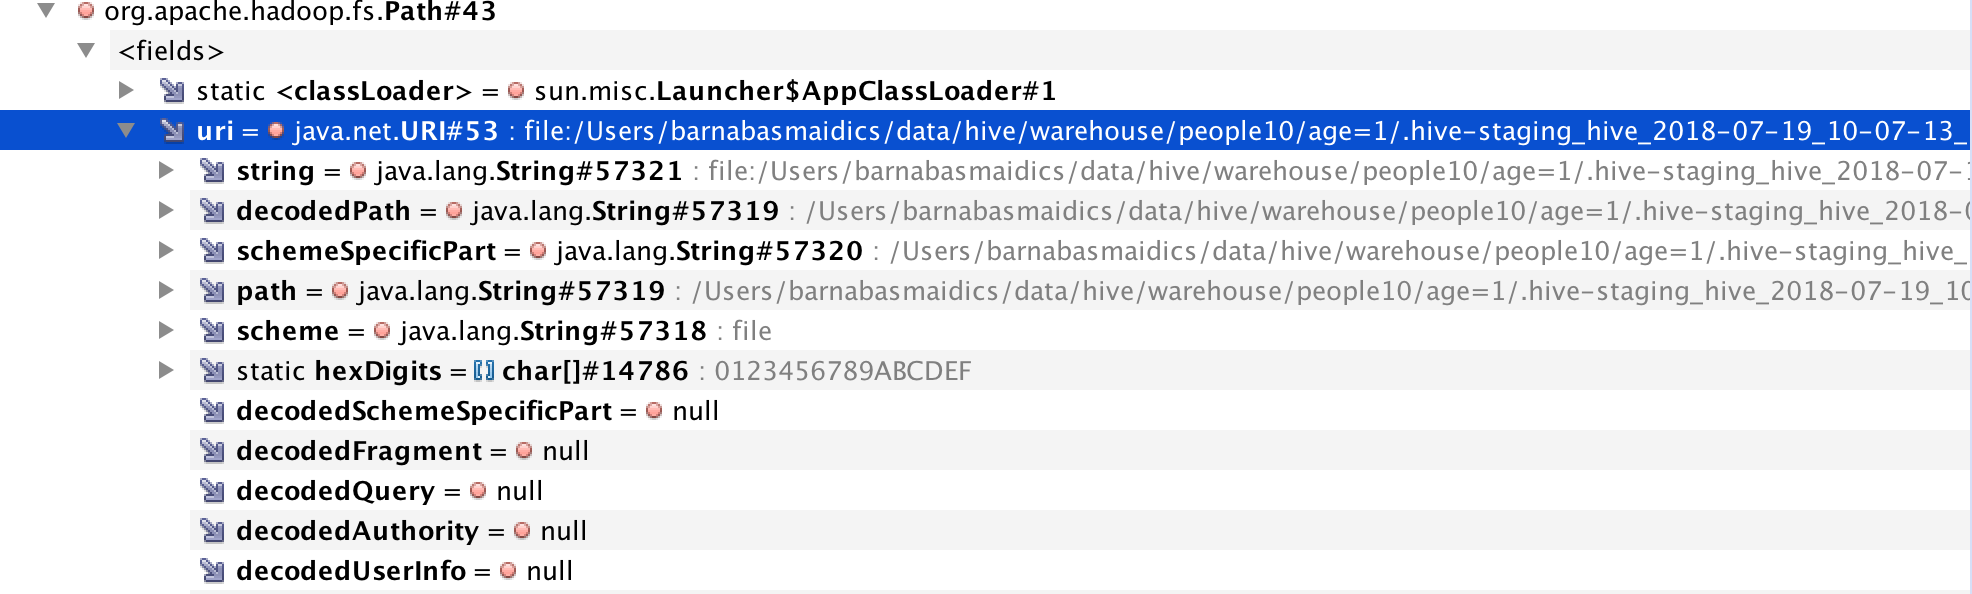
\includegraphics[width=150mm, keepaspectratio]{figures/path_memory.png}
	\centering
	\caption{Inside of a Path}
\end{figure}

In Path objects, we store the location in a \textit{java.net.URI} object. Its internal representation seems really wasteful. As we see, URI stores a path in 3 different Strings. The Strings are almost the same: for example the string field inside the URI contains the scheme, the path field does not, and this is the only difference \etc. We can ask ourselves: is it really necessary?

To determine this we need to inspect the Path.java source code. URIs are always created the same way: we pass four String parameters to the constructor of the URI class: scheme, authority, path, and fragment. In the code below the null parameter represents the query part of a URI. Passing null means that we do not need that value.

\begin{lstlisting}
	newUri = new URI(scheme, authority , path, null, fragment);
\end{lstlisting}

To summarize, the internal representation of the URIs clearly seems like a waste of memory. So I started to think of an alternative solution to replace these URI objects and save around 66\% of memory for each Path. 

\chapter{Fixing memory waste of URIs - HDFS-13752}
The duplication comes from the \textit{java.net.URI} objects so the first thing that came to my mind was to replace this with a more memory efficient implementation in the Path.java class. As a first approach, I created a Jira ticket in the corresponding Apache site to report the issue \cite{hdfs-path}. 

The community agreed that the way URIs store these paths is a waste, and could be stored more efficiently. However, many other classes use these URIs. The Path class has a public \textit{toURI} function which returns the URI representation of the path. Obviously, this cannot be removed because others are depending on it. I found three possible solutions to get rid of this memory overhead.

\begin{itemize}
	\item Keep the URI field with only having a WeakReference to it, and store the 4 parts of the Path in seperate fields
	\item Keep the URI field with only having a SoftReference to it, and store the 4 parts of the Path in seperate fields
	\item Remove the URI field completely and store those parts of the URI that we really use in separate Strings
\end{itemize}
\section{Solution ideas}
\subsection{Solution 1: WeakReference}
A WeakReferenced object works in a way, that if the object is only weakly reachable (its only reference is a WeakReference), it will not prevent the object to be garbage collected. We would have a WeakReference to the URI and when the GC runs it can collect the URIs if we do not have a strong reference to it. 

When someone wants to get the URI representation of the path and calls the \textit{toURI} function, we need to check if the URI exists through the WeakReference or not. If it exists we can just get it because we have a WeakReference to it. If it does not, we need to recreate the URI from its parts. 

\subsection{Solution 2: SoftReference}
Using SoftReference would be a more conservative solution. If the Garbage Collector finds an object that is only softly reachable, it does not dump the object instantly. An object with a SoftReference will only be collected at memory demand. This way before an Out Of Memory error is thrown, the GC can free all URIs. If the GC collected the URI we would do the same as mentioned before: recreate the URI from the stored parts when needed. 

\subsection{Solution 3: On demand URI creating}
A possible solution is to remove the URI completely and only keep 4 parts of the Path which are used: scheme, authority, path and fragment. This way we can immediately win around 66\% of memory. The only drawback is that we always have to recreate the URI every time the toURI method is called and this might be expensive CPU-wise.

\begin{figure}[H]
	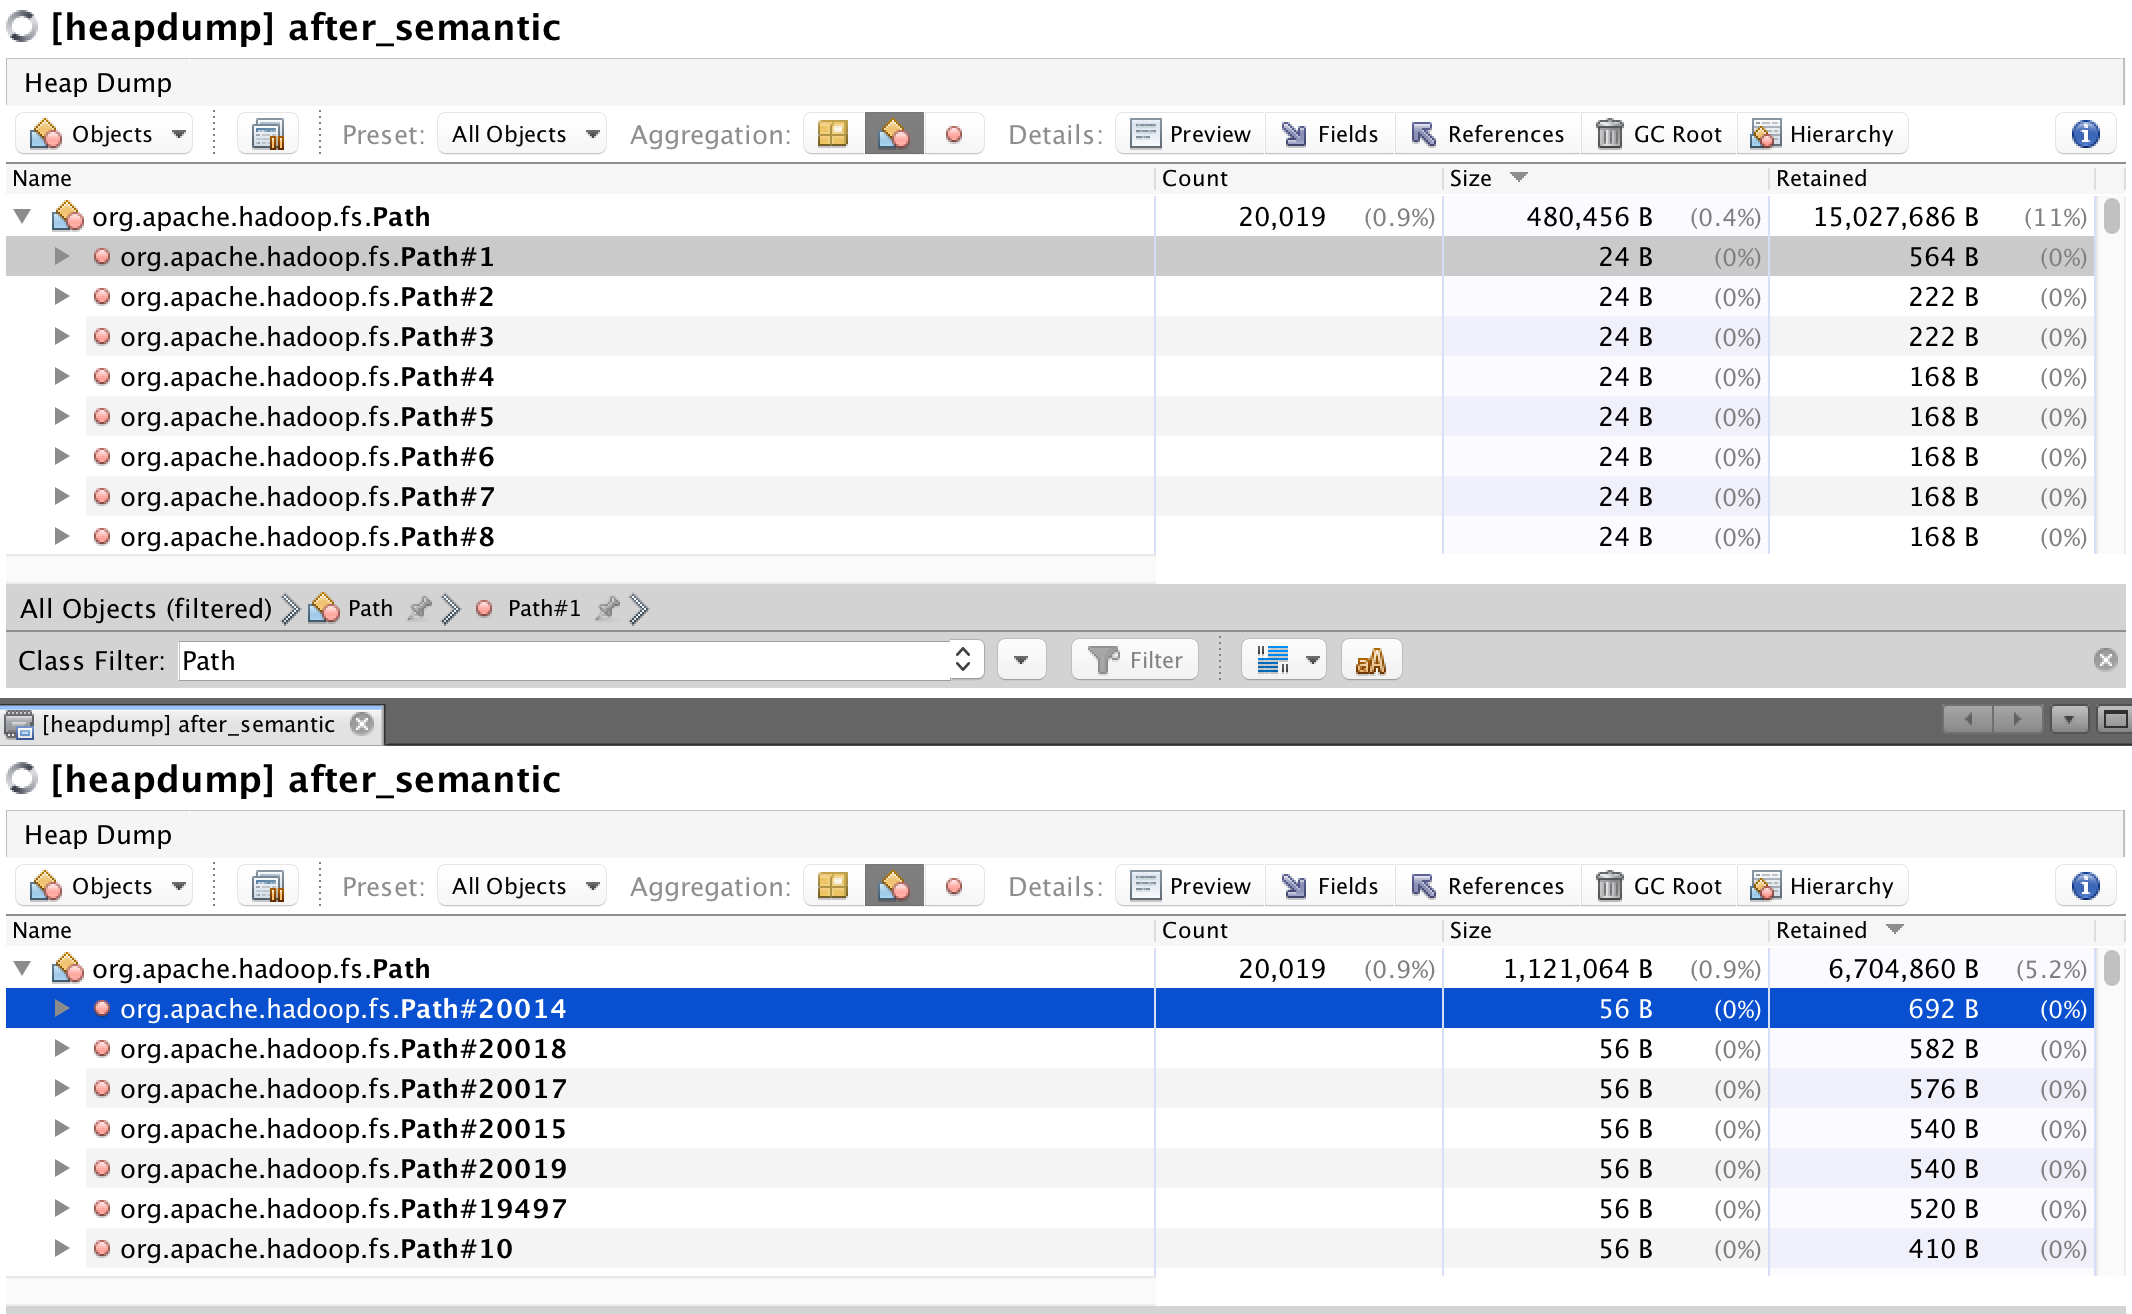
\includegraphics[width=150mm, keepaspectratio]{figures/path_before_after.png}
	\centering
	\caption{Memory save of Paths}
\end{figure}

\subsection{Conclusion}
For the second thought, I realized that using WeakReference would not be the best decision. It would almost be the same as creating the URI on demand, since whenever the GC runs, it will collect the URIs immediately and when toURI is called we would have to recreate it anyway. The only way to decide which solution might be the best is to measure the performance of both approach. 

I also analyzed the code base of Hadoop to see how \textit{Path.toUri} method is usually used. Most often we just want to ask for certain parts of the Path object and not really using the URI itself. For example: \textit{pathObject.toUri().getPath()} to get the path or \textit{pathObject.toUri().getScheme()} to get the scheme. Considering only this, solution 3 would be the most effective, since we are able to get the path/scheme/authority or fragment directly from the Path object and we do not need to first transform it to an URI and than ask for the value we need. 

\section{A simple performance test for toURI}
I created a really simple test, to decide which solution would solve the issue without a significant CPU overhead. 

I tested the CPU usage of the toUri() method, analyzing the different solutions: I created 1.000.000 Path objects (of course this is not a real use case, but it can be a good estimation as the first approach). See the results in the table below (3. row). I’ve also measured the memory effects of the changes. 

\noindent The code I used for testing:
\begin{lstlisting}
long startTime = System.nanoTime();
for(int i=0; i<1000000; i++){
	paths[i].toUri().getPath();
}
long estimatedTime = System.nanoTime() - startTime;
\end{lstlisting}

\begin{table}[H]
	\begin{tabular}{|l|l|l|l|}
		\hline
		& \textbf{Original} & \textbf{\begin{tabular}[c]{@{}l@{}}SoftReference \\ (solution 2)\end{tabular}} & \textbf{\begin{tabular}[c]{@{}l@{}}New URI \\ (solution 3)\end{tabular}} \\ \hline
		\textbf{Memory of the Paths}     & 608 MB            & 664 MB                                                                         & 238 MB                                                                   \\ \hline
		\textbf{Time of the toURI calls} & 0.12973 s         & 0.04142 s                                                                      & 1.29133 s                                                                \\ \hline
	\end{tabular}
\centering
\caption{Results of the test}
\end{table}

The results showed that using SoftReference has a bit of memory overhead because apart from the URI itself, we need to store the SoftReferences which require heap space as well. Thus, it would only be a save if the heap is almost full, other than that we it would reserve even more memory. The time of toURI calls might be deceptive. Calling \textit{toURI} method only once is slower than with the original solution and we do not use the method as in the example above. 

Looking into the results of the third possible solution, the benefits are clear memory-wise. However, the time of the toURI calls do not look so promising. The CPU time is almost 10x bigger than with the original approach. But if we take into account other factors, not just the plain CPU time, the overhead might not be that big. If the memory of the paths are reduced, the GC can work much faster, so smaller GC pauses will occur. Also, these Path objects passed through the interface of Hadoop in both direction. For example, NameNode gives the location of files in the format of Paths and Hive passes these objects to Hadoop as well. Considering these, my change would be possibly beneficial for transfering data through the network: Passing objects which are smaller is obviously faster. 

An additional factor that should be considered is that if we remove the \textit{toUri} call whenever we want to get the values of path, scheme, authority or fragment, we can improve the performance of the original solution, since we can get those directly. Instead of \textit{Path.toUri().getPath() } we can just say \textit{Path.getPath()}.

To test this theory, I created a simple test. The times of 1.000.000 toUri().getPath() calls:
\begin{itemize}
	\item Original: 0.143235527 s
	\item Solution 3 if Path.toUri().getPath() staying: 1.316882214 s
	\item Solution 3 with only Path.getPath(): 0.004373138 s
\end{itemize}

With the results of my test, I decided to choose solution 3, which may be the simplest fix: remove the URI field completely and if someone needs it, create on demand from the path, scheme, authority and fragment parts.

\section{Performance test on a cluster}
As a next step, I configured a cluster to see if my change would affect CPU significantly. The cluster I created had 4 nodes and only HDFS, YARN and HIVE were installed. I generated the below HDFS directory structure to test the performance of my fix. The "perftest" directory contains 100 folders, each contains 1000 other folders with one txt file. The code I used for testing can be found in the Jira ticket I reported \cite{hdfs-path} (HDFS-13752.003.patch).

\begin{figure}[H]
	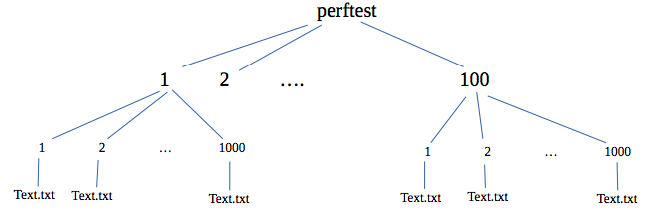
\includegraphics[width=125mm, keepaspectratio]{figures/directory_structure.png}
	\centering
	\caption{Directory structure of the test}
\end{figure}

For the tests, I used FileSystem shell to interact with the HDFS directly. I choosed one shorter and one longer running operation for measuring the CPU time. The values in the tables are in millisecond.

\subsection{Listing files recursively}
The command used:  \textit{hdfs dfs -ls -R /user/perftest}

\begin{table}[H]
	\begin{tabular}{|l|l|l|l|l|l|l|}
		\hline
		& \textbf{M1} & \textbf{M2} & \textbf{M3} & \textbf{M4} & \textbf{M5} & \textbf{Avg} \\ \hline
		\textbf{Original} & 42651    & 38136    & 40183    & 41749    & 36963    & 39936     \\ \hline
		\textbf{New URI}  & 41762    & 39219    & 38800    & 37315    & 37719    & 38963     \\ \hline
	\end{tabular}
\centering
\caption{CPU time of a recursive listing}
\end{table}
\subsection{Changing the replication factor of a file}
The command used:  \textit{hdfs dfs -setrep -w 3 /user/perftest}

\begin{table}[H]
	\begin{tabular}{|l|l|l|l|l|l|l|}
		\hline
		& \textbf{M1} & \textbf{M2} & \textbf{M3} & \textbf{M4} & \textbf{M5} & \textbf{Avg} \\ \hline
		\textbf{Original} & 172240      & 179050      & 193963      & 189105      & 171446      & 181161       \\ \hline
		\textbf{New URI}  & 185523      & 169111      & 171326      & 171451      & 170389      & 173560       \\ \hline
	\end{tabular}
\centering
\caption{CPU time of a replication factor changing}
\end{table}

\subsection{Analyzing the results}
Seeing the results I think there is no big performance difference. The new solution is even a little bit faster. A possible explanation for this is that I removed several \textit{toUri()} calls inside the Path class, because we store the Path, Scheme, Authority and Fragment in the Path object. These can also be done outside of the Path class. Another explanation can the network improvement mentioned before or even the decrease of the GC pauses. Or it may only be just the inaccuracy of the measurement.

\section{Effects of the change in Path}
After publishing the results to the Apache HDFS Jira, I tried to investigate if the change would be really beneficial. These Path objects can be found in every component that uses Hadoop, like Hive, Impala, HBase \etc and used widely everywhere in the code. As a consequence of this, a little CPU overhead can even cause a big performance loss so the patch needs to be tested throughly. 

If this little change has some possibility to decrease the performance significantly, would it really benefit the components? I did an investigation to see if this issue is real and what would it fixed. Based on the results, my answer is: yes. The following issues was partly or entirely caused by the size of memory these Path objects reserve, so reducing the size with 66\% may solve or help these problems.

\subsection{Hive MetaStore OOM}
During my investigation I found a HMS memory issue in production use of Hive. The MetaStore server crashed due to an Out Of Memory error. The following heap dump was created before the OOM. Here 9.743 Gigabytes of memory was used by \textit{fs.Path} objects.

\begin{figure}[H]
	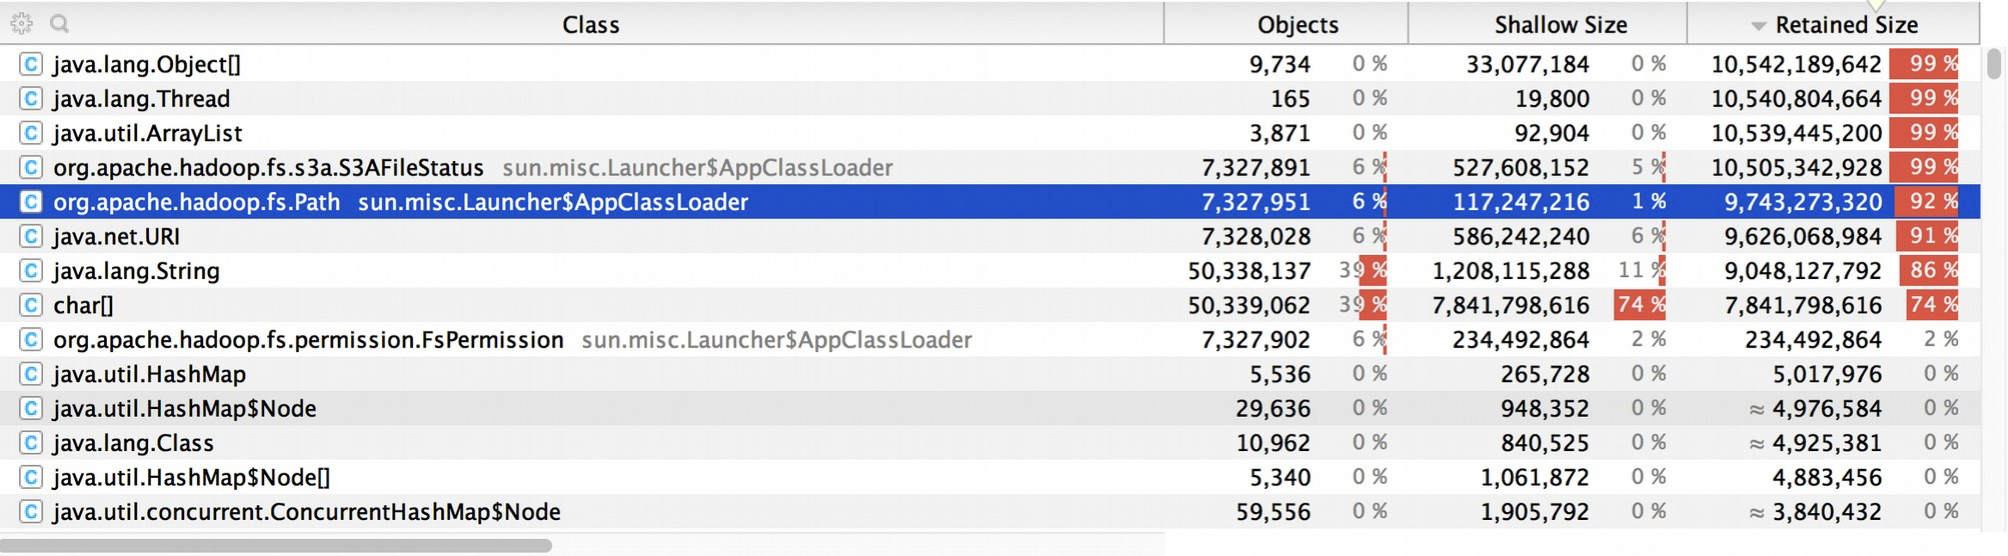
\includegraphics[width=150mm, keepaspectratio]{figures/hms_heapdump.png}
	\centering
	\caption{HMS heap dump before OOM}
\end{figure}

\subsection{Hive on Spark memory issue}
Stress testing of HoS (Hive with Spark execution engine) has revealed that we have memory issues when running with a high value of \textit{spark.executor.cores}. The overhead is mainly introduced by loading multiple copies of HiveConf (Hive configuration object) and there is a significant overhead when loading lots of Path objects too. In the next chapter I will focus on the multiple HiveConf issue as well.

\subsection{"Small files problem" in HiveServer2}
HS2 has a so called "small files problem". Something like \textit{create external table} with lots of small files in the  HDFS directory of the table causes HiveServer2 to load the HDFS paths of the files into memory. If we have millions of small files (which is not that rare), these paths can use Gigabytes of heap memory. Hive does a \textit{listFiles} that returns all the Paths, to determine file permissions \etc. So create table hangs and other queries wait a LOT.

\subsection{Apache Impala's solution for the problem}
Apache Impala also faced problems caused by the size of memory used by the Paths. Impala is a query engine on top of Hadoop, similar to Hive. They already solved this problem on their side. Impala has a \textit{HdfsPartitionLocationCompressor.java} class which they use to solve exactly this problem. I also thought of the idea to solve the issue in Hive, however for a long term, it may not be the most desirable strategy. Hive would have to always convert the Paths whenever it passes them to Hadoop (Impala does this). I think if the problem can be solved in  Hadoop - where it comes from - without a performance overhead, it should be done there. My task is to give the community a proof that CPU overhead will not happen because of the memory fix. 

\section{Benchmarking on a data center cluster}
The patch would effect every part of Hadoop, so a thorough benchmark is needed. The performance tests run on a data center cluster with Hadoop 3.0.0 for more than a month. From 13 September to 25 September without my patch, from 26 September to 19 October with my patch. The following charts will show the results for some test cases. On these diagrams, the values before the red line are without my patch and after the red line are the values including my patch. I created several diagrams to show the full result to the community. I will only include a part of them here, the full document can be found on the Jira ticket (HDFSbenchmark.pdf) \cite{hdfs-path}.

\noindent Parameters of the benchmarks: 
\begin{itemize}
	\setlength{\itemsep}{1pt}
	\item Number of worker nodes: 7
	\item Dataset size per node: 1000 GB
	\item Number of mappers per node: 80
	\item Filesize for TestDFSIO: 16 GB
	\item Number of files for NNBenchmark: 50000
\end{itemize}

\subsection{TeraSort benchmark}
"TeraSort reads the input data and uses MapReduce to sort them." \cite{terasort}

\begin{figure}[H]
	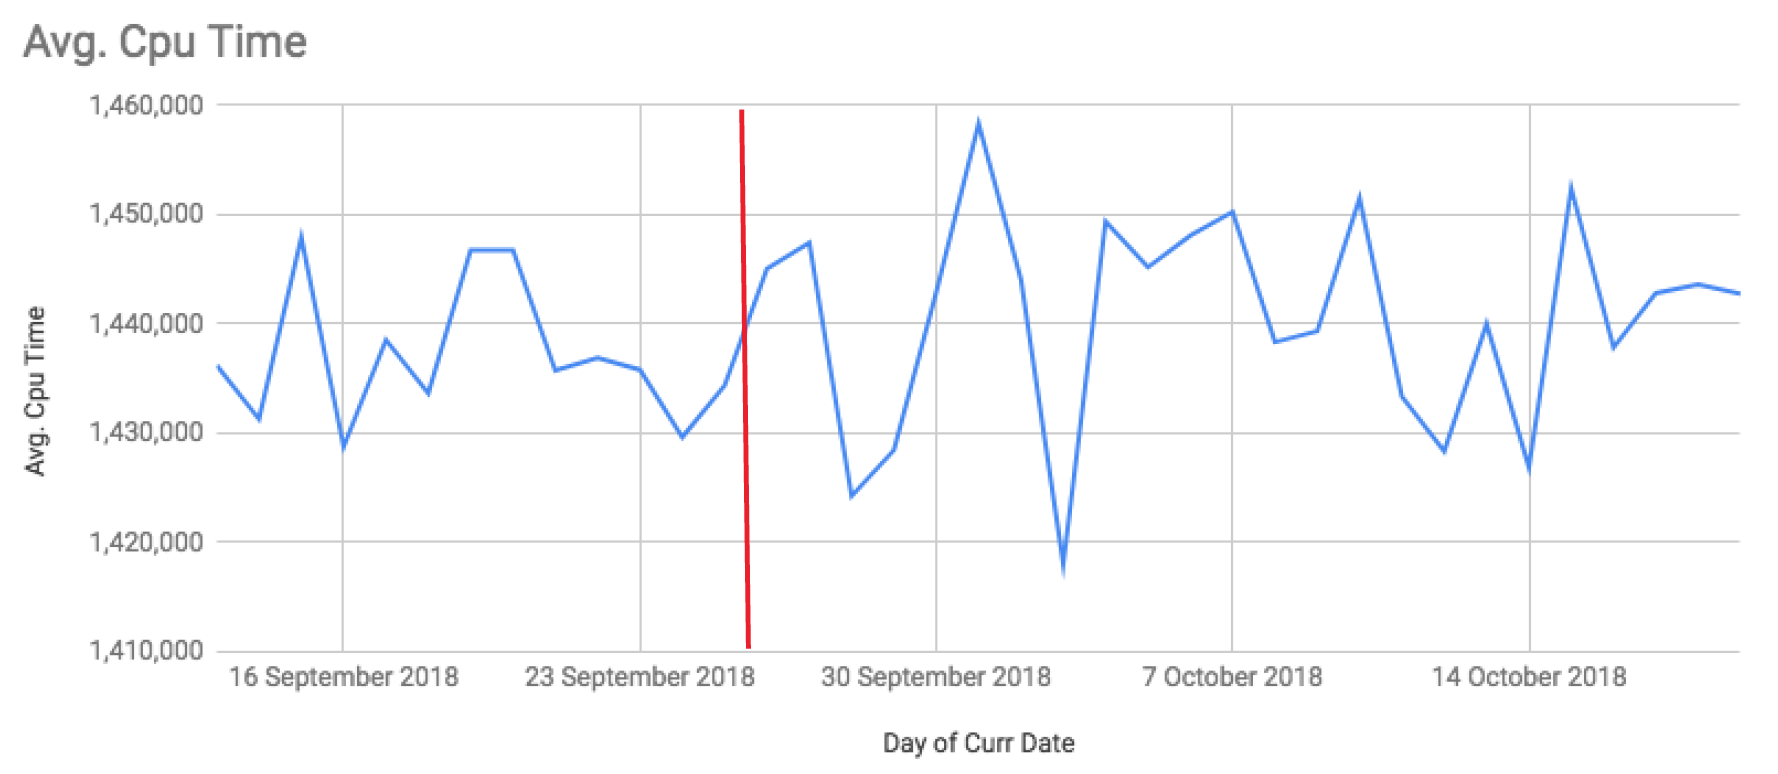
\includegraphics[width=125mm, keepaspectratio]{figures/terasort_cpu.png}
	\centering
	\caption{TeraSort Average CPU time}
\end{figure}
\begin{figure}[H]
	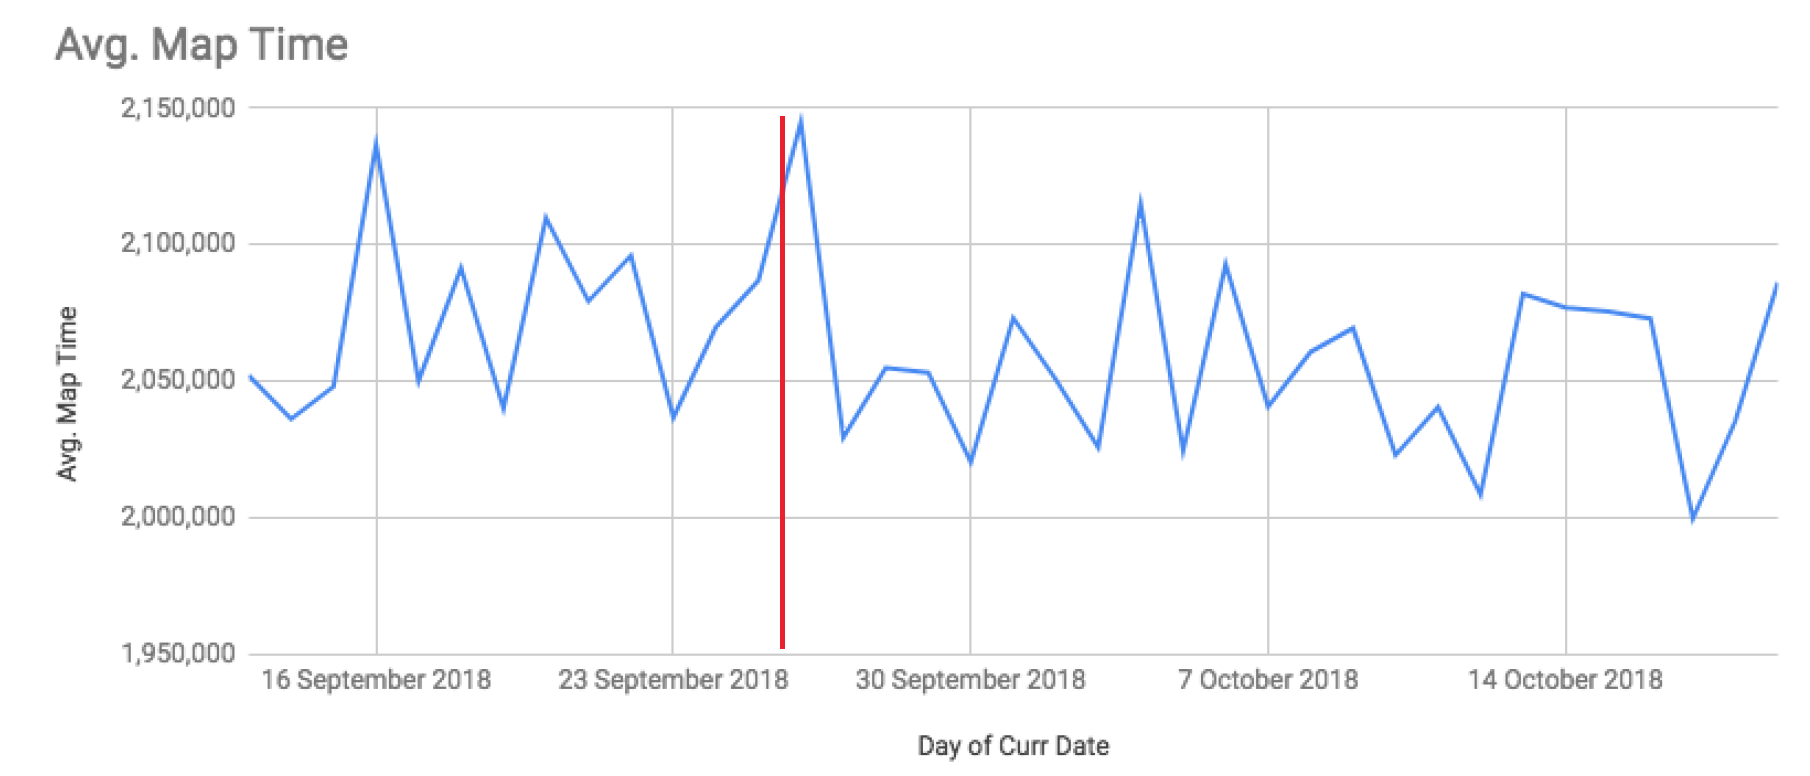
\includegraphics[width=125mm, keepaspectratio]{figures/terasort_map.png}
	\centering
	\caption{TeraSort Map time}
\end{figure}
\subsection{TeraValidate benchmark}
"TeraValidate validates the sorted output to ensure that the keys are sorted within each file. If anything is wrong with the sorted output, the output of this reducer reports the problem." \cite{terasort}

\begin{figure}[H]
	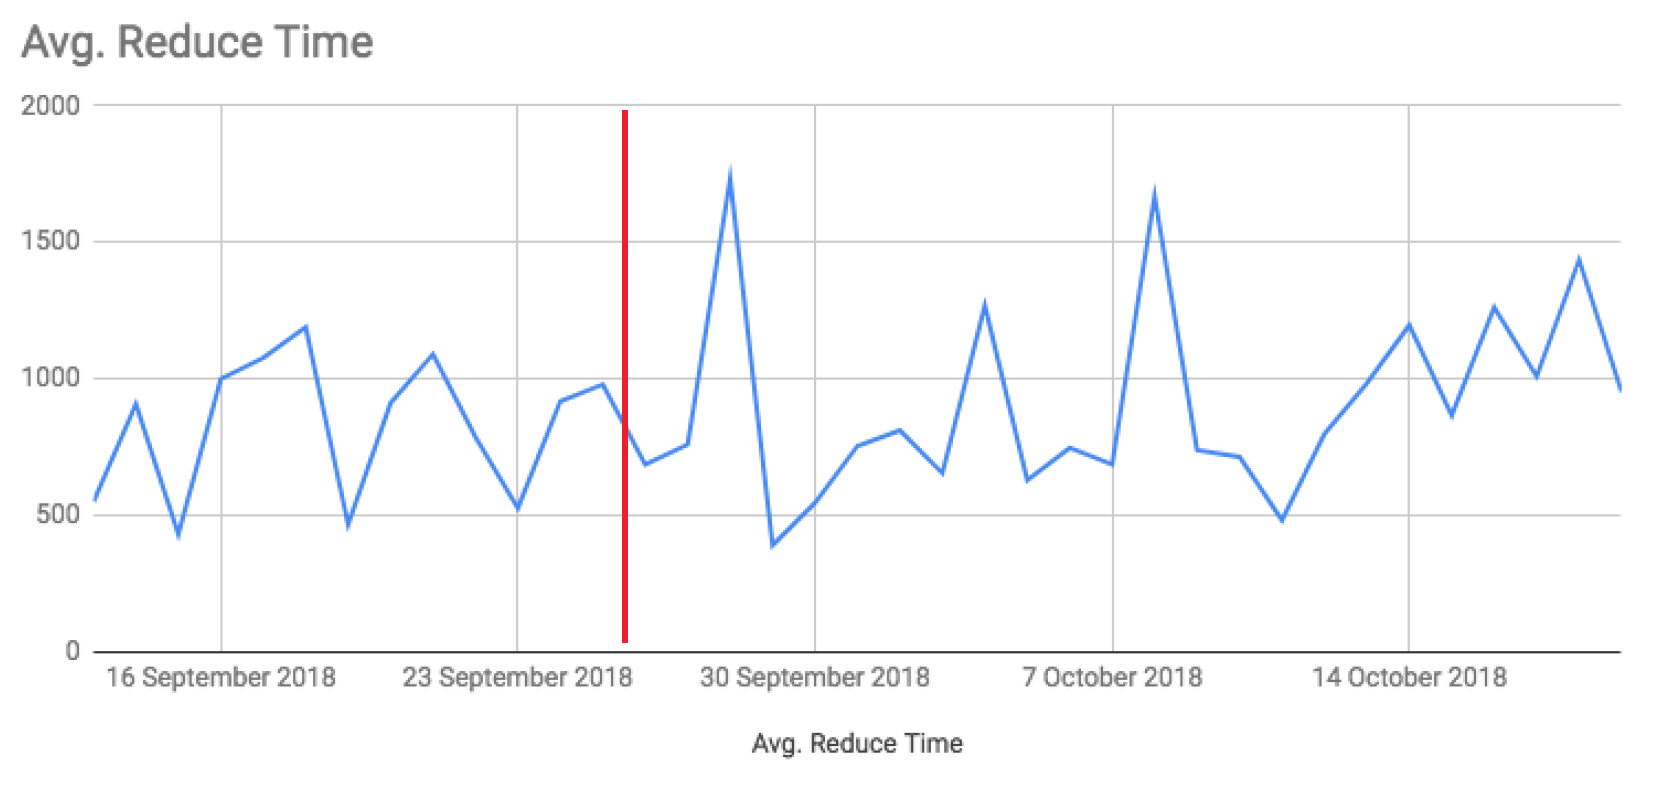
\includegraphics[width=125mm, keepaspectratio]{figures/teravalidate_job.png}
	\centering
	\caption{TeraValidate Job time}
\end{figure}
\begin{figure}[H]
	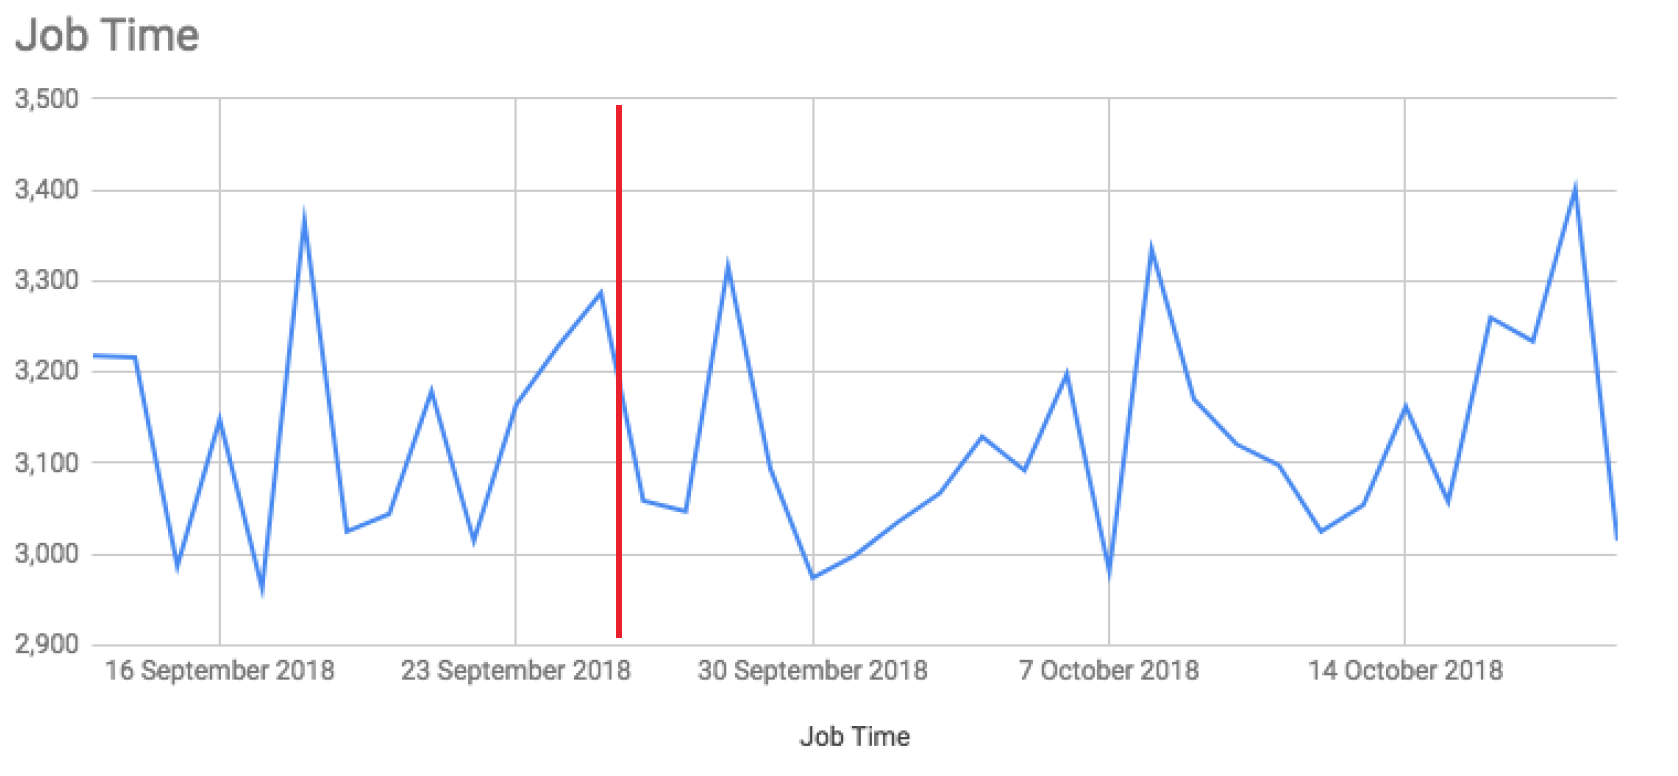
\includegraphics[width=125mm, keepaspectratio]{figures/teravalidate_reduce.png}
	\centering
	\caption{TeraValidate Reduce time}
\end{figure}

\subsection{TestDFSIO}
TestDFSIO is a benchmark for measuring the capacity of HDFS for reading and writing data. It is helpful to discover performance bottlenecks.

\begin{figure}[H]
	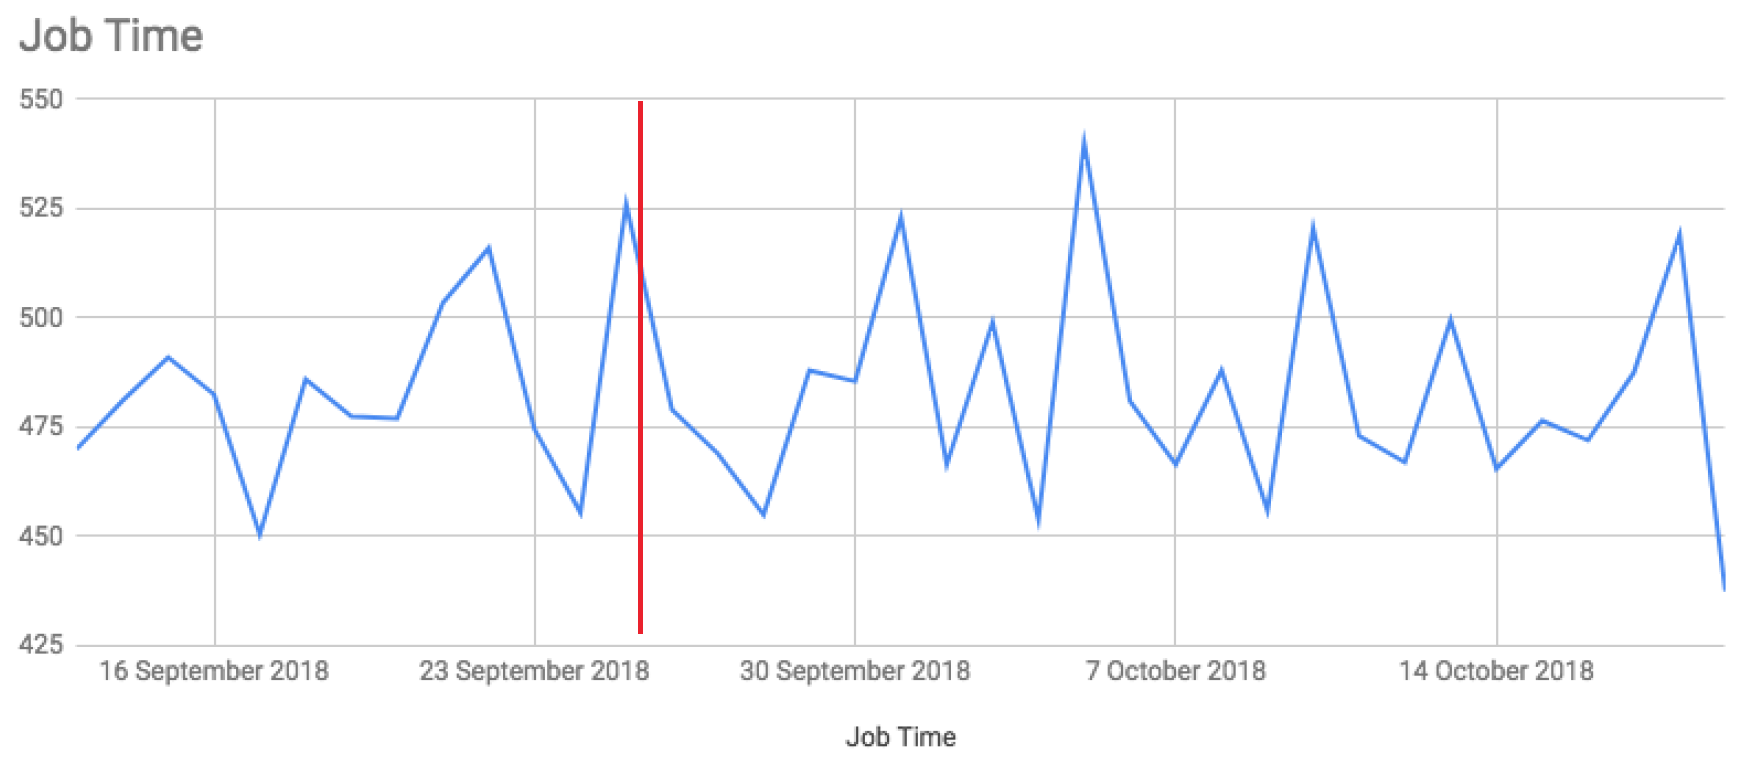
\includegraphics[width=125mm, keepaspectratio]{figures/dfsio_job.png}
	\centering
	\caption{TestDFSIO Job time}
\end{figure}

\subsection{NNBench - NameNode stress test}
This benchmark generates a lot of HDFS requests for putting a high HDFS management stress on the NameNode. The benchmark can create, read, rename and delete files on HDFS.

\begin{figure}[H]
	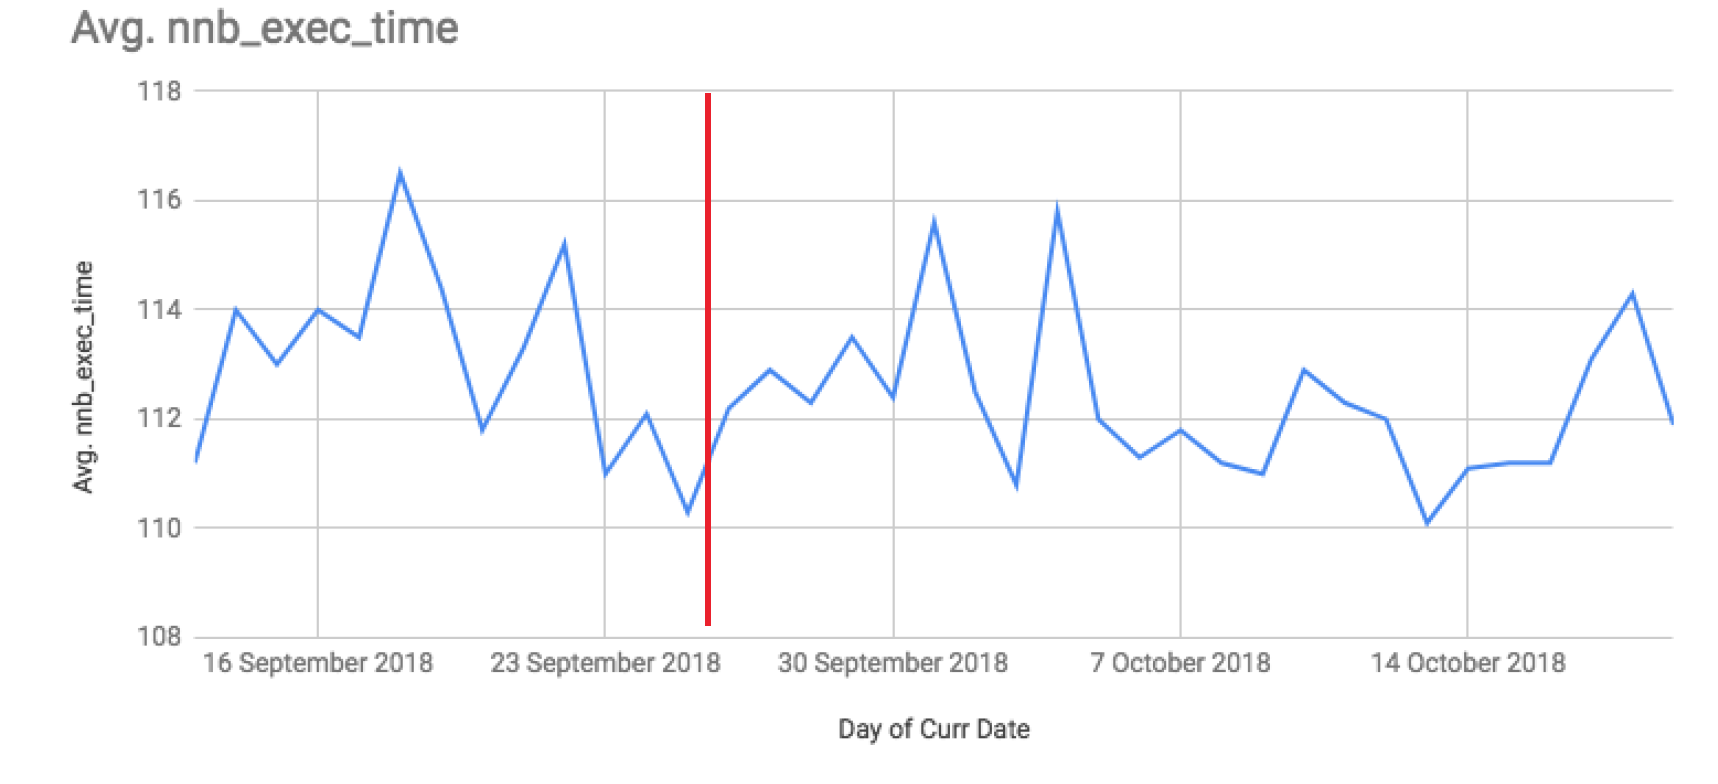
\includegraphics[width=125mm, keepaspectratio]{figures/nn_exec.png}
	\centering
	\caption{NameNode execution time of open\_read operation}
\end{figure}
\begin{figure}[H]
	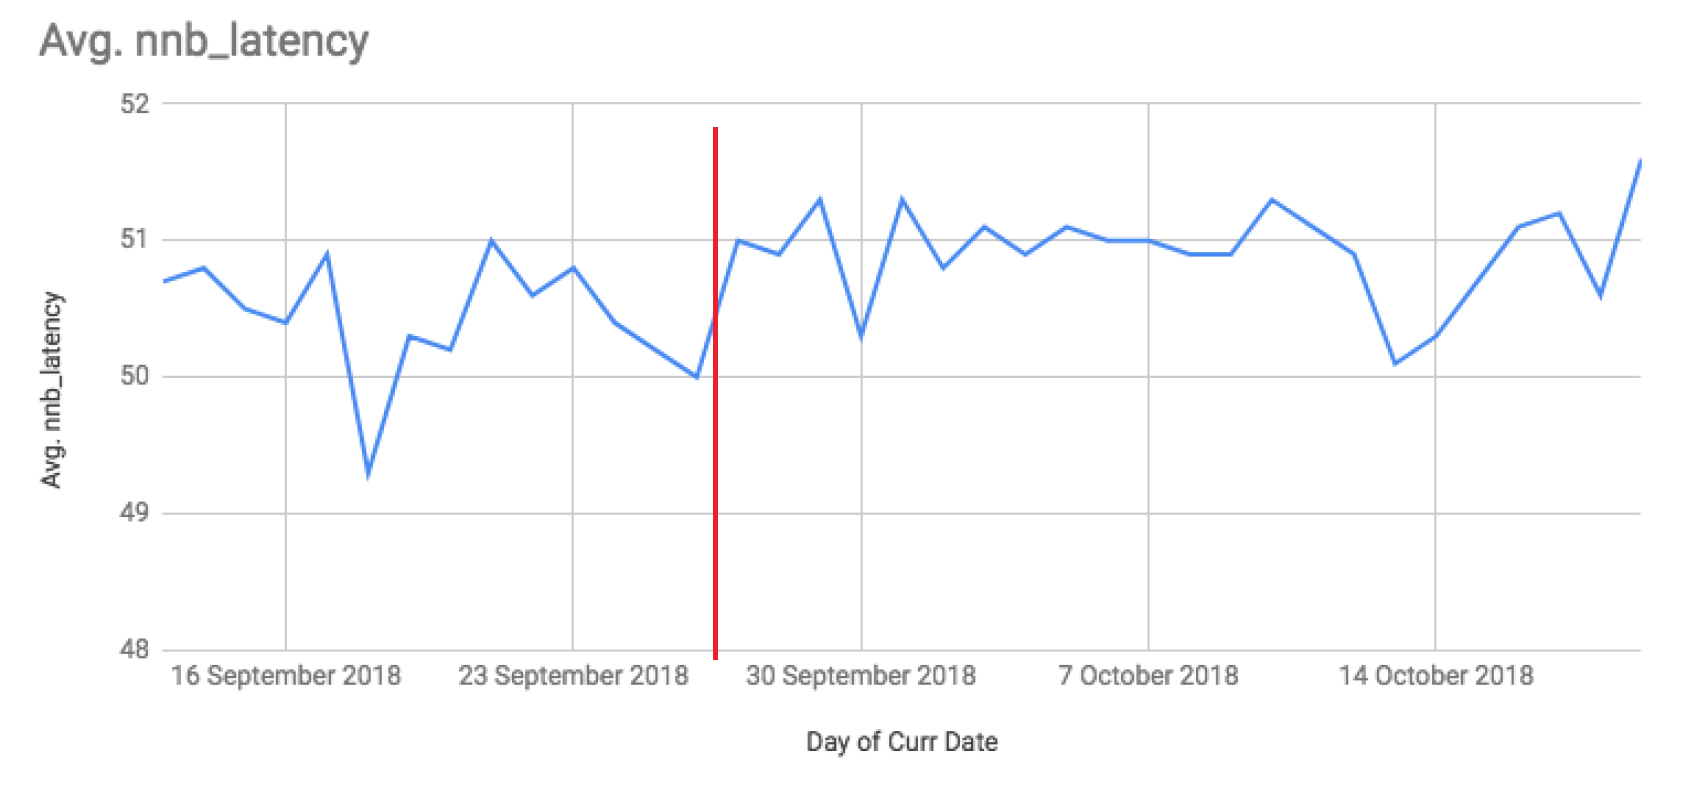
\includegraphics[width=125mm, keepaspectratio]{figures/nn_latency.png}
	\centering
	\caption{NameNode latency of open\_read operation}
\end{figure}

\section{Result of the benchmark, further tasks}
Looking into the charts and comparing the results of the base (before the red line) and the results with the patch included (after the red line), we cannot see any significant difference in CPU time, so this benchmark gave a positive outcome. 

Since the fix would affect many other components, more benchmarks are still needed to be certain that this will not decrease the perfomance of Hadoop. Hive benchmark is currently in progress to see if any performance bottleneck is introduced on the "client" side by changing the implementation of Paths.

\chapter{Another memory issue in Hive - HIVE-20760}
It is known, that Hive memory depends on mainly two factors: one is the number of partitions in tables and the other one is the number of connections made to HiveServer2. In the first part of my work I focused on the number of partitions and found a way that would decrease the memory of HiveServer2 when our tables are highly partitioned. In this section I will try to get a better understanding what uses so much memory when multiple connections are made and see if the issue can be fixed or not. 

\section{Memory of HS2 with multiple connections}
HiveServer2 can serve multiple clients at the same time. Obviously, the resources needed for handling multiple connections is proportional with the number of client connected to the server. Let's see what uses memory in this scenario.

I wanted to see the memory effect of the number of connections only, so I decided to analyze the memory before compilation and execution happens. This way I can get a clearer picture, since memory used by compilation or execution will not be presented, only the overhead of each connection. 

For each connection made to Hive, a session is created. I use a bash script for simulating multiple clients connection to Hive locally. 

\begin{lstlisting}
#!/bin/sh
for i in `seq 1 50`; 
	do <location of beeline>/bin/beeline -u jdbc:hive2://localhost:10000 -n admin -p admin -e "select count(*) from people200;" 
&done;	
\end{lstlisting}

In the body of the for loop, for each iteration I made a connection to HiveServer2 using Beeline command line client. As arguments, I provided the jdbc connection URL of HS2 (the default port HS2 is listening is 10000) and the username/password, which is admin/admin as a default value.

With the previously mentioned measuring code, I created a heap dump after 50 connections were made to HS2 and sesssion were already created. The following figure shows the objects that use the most heap memory.

\begin{figure}[H]
	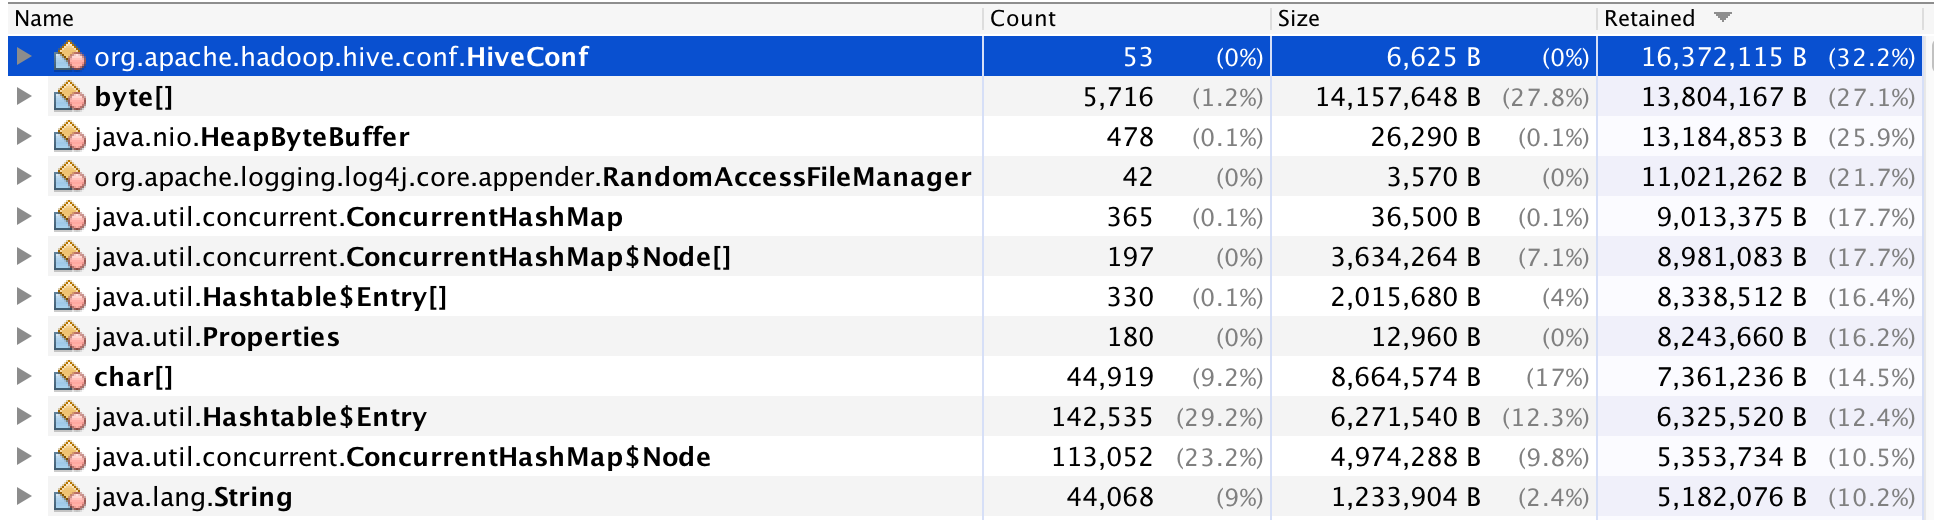
\includegraphics[width=150mm, keepaspectratio]{figures/hiveconf_memory.png}
	\centering
	\caption{Object with the most retained memory}
\end{figure}

For each session, an individual HiveConf object is created, which contains all the configuration properties of Hive. These configurations can easily contain thousands of values so the big heap memory is not that surprising. The first thing I recognized during the analyzis of the heap dump, is that each HiveConf object of a session use the same amount of memory. Thus, these objects cannot be that different from each other. If that is the case, why do we have a different one for every session?

The HiveConf class is a descendant of the \textit{Configuration.java} class, that is inherited from Hadoop. The biggest memory of each HiveConf a private Properties field. The Properties class is a type of HashMap that only contains String keys and values. Looking into the Properties fields of each HiveConf confirmed my assumption: they have exactly the same values apart from a few properties.

This inspired me to look more into the details. How these configuration objects are used? When we start Hive, Hadoop configuration properties are applied, and we read Hive's configuration file (hive-site.xml) and overlay those properties. After this, for each session we create a new HiveConf instance with copying the existing "base". This way sessions can add their own unique Properties to their configuration object. 

It is important to notice that we rarely touch the "base" configurations. Usually the sessions add some Properties to it and the base configuration remains untouched. To get rid of the memory overhead, a possible solution would be to use the same Properties object for each HiveConf if the values in them are the same.

\section{HIVE-20760: Reducing memory overhead due to multiple HiveConfs}
I already saw a somewhat similar problem, when looking into the partition memory issues. PartitionDesc used exactly the same Properties object, and the solution for that was introducing CopyOnFirstWriteProperties class \cite{hive-partitions}. 

It is a special subclass of Properties, designed to save memory when lots of identical Properties are created. The class uses interning to solve the problem: it has an interned Properties field which points to the same object for all instances that has identical contents. If any mutating method (\eg setProperties, put, clear) is called on the object, the content is copied to "this" instance, and we no longer use the interned object. 

As a first idea, I thought that using this class would help. However, HiveConfs are used differently from PartitionDesc, and this solution was desinged for that. We often call mutating methods on the Properties field of HiveConf. Each session is able to add additional values to its configuration. Thus, other solution is needed to save memory in this scenario, since using CopyOnFirstWriteProperties immediately throws away the interned Properties if we add a new property to it.

\subsection{Introducing HiveConfProperties class}
My idea was to intern only the "base" Properties. When we create a HiveConf from an already existing one using its "copy constuctor", instead of creating a built in \textit{java.util.Properties} we will use a subclass of Properties. I named this class HiveConfProperties. 

I designed HiveConfProperties to save memory caused by the many nearly individual HiveConfs. Right after we create a HiveConfProperties instance, from an already existing Properties, we can intern that. For interning, I used \textit{com.google.common.collect.Interner}. 

\subsubsection{How interning works} 
 When we have an object that we want to intern, we search for it in the "object pool" to see if there is already an object equal to the corresponding one. If we find one, we will use that in the future. If there is no object equal to the actual one then we put the object into the pool and then use it. Fortunately, there is already an existing implementation of this interning method in the Google Guava core java library.
 
 \subsubsection{How HiveConfProperties works}
 I divided the Properties object into two parts: an interned part, which contains the base Properties, and since we descend from \textit{the java.util.Properties}, we can use the "this" object to store properties as well.
 
 \begin{figure}[H]
 	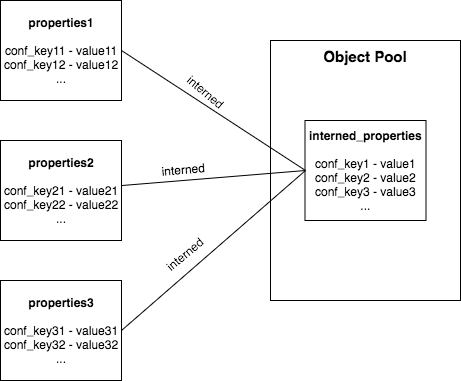
\includegraphics[width=100mm,keepaspectratio]{figures/hiveconf_solution.png}
 	\centering
 	\caption{How HiveConfProperties works}
 \end{figure}

\begin{lstlisting}
private Properties interned;

private Properties removed;
private int duplicatedPropertiesCount;

private static Interner<Properties> interner = Interners.newWeakInterner();

public HiveConfProperties(Properties p) {
	if(p != null) {
		interned = interner.intern(p);
	}
	removed =  new Properties();
	duplicatedPropertiesCount=0;
}
\end{lstlisting}

The code above is responsible for creating a HiveConfProperties instance. It stores the interned (base) Properties in a private field. Right after we want to construct an instance, we intern the given Properties object. The process that \textit{interner.intern(...)} does is explained above. A null check is also a must when we create a new HiveConfProperties, since calling the constructor with null parameter is possible in the code. I found this possibility when I submitted the patch to Apache Hive Jira and "PreCommit" tests failed during the Jenkins build. The \textit{removed} and the \textit{duplicatedPropertiesCount} field is needed for the interning to work as expected. 

If someone calls \textit{HiveConf.unset} funciton, \textit{Properties.remove} (this case \textit{HiveConfProperties.remove} will be called. If the property we want to remove is contained by the interned Properties object, we cannot remove it directly, because other HiveConfProperties may use it. To solve this issue, I introduced the \textit{removed} Properties field to store those values that should no longer be available. So if we want to get the value of a key, we first check if the key is in the \textit{removed} Properties: if the answer is yes, we will consider this property unavailable.

Duplications can occur in my solution: if someone would like to set a property, that is already in the \textit{interned} field, we cannot override it there, so we should add it in the non-interned Properties to return the correct value. However, this way we will have two properties with the same content. Calculating the size of the HashMap will be inaccurate. For solving this issue, I created a counter field called \textit{duplicatedPropertiesCount} to store the number of the duplicates. Knowing this value will allow us to provide an accurate size. 

Since HiveConfProperties is a subclass of \textit{java.util.Properties} and because of it subclass of \textit{java.util.HashTable}, I provided implementation of its methods.  \textit{hadoop.conf.Configuration} (base class of HiveConf) and \textit{HiveConf} only uses a subset of these functions, so I decided to implement only those, that can be invoked. For the other methods I will throw a \textit{NotImplementedException}. 

\subsection{Overriden functions of Properties}
\subsubsection{getProperty}
\begin{lstlisting}
@Override
public String getProperty(String key) {
	String property = super.getProperty(key);
	if (property == null) {
		if(interned != null && !removed.containsKey(key)) {
			property = interned.getProperty(key);
		}
	}
	return property;
}
\end{lstlisting}

If non-interned (super) contains the key, return that value. If not, we need to check if it is not in the \textit{removed} Properties (still valid). If the value is valid, return it from the base (interned). \textit{getProperty(String key, String defaultValue)} and \textit{get} method from HashTable works the same way. 
\subsubsection{setProperty}
\begin{lstlisting}
@Override
public synchronized Object setProperty(String key, String value) {
	if(interned != null && interned.containsKey(key) && !super.containsKey(key)) {
		String internedValue = interned.getProperty(key);
		if(internedValue.equals(value)) {
			return internedValue;
		}
		duplicatedPropertiesCount++;
	}
	//If removed contains this key, and we want to set it, it is no longer "removed"
	if(removed.containsKey(key)) {
		removed.remove(key);
	}
	return super.setProperty(key, value);
}
\end{lstlisting}

If interned already contains the property to be set, we need to set it in the non-interned Properties. However, this way we will have duplicates, since both Properties instance will contain the same value. Thus, to be able to give a correct size when needed, we need to count these duplicates. If we are setting a value, that had been removed previously, we need to "revalidate" the property. If the value is not changed, we should not set it in the non-interned Properties to avoid unnecessary duplicates. 

\subsubsection{mergeProperties helper function}
To override functions such as \textit{stringPropertyNames} or \textit{keySet} \etc I introduced a helper function. Since for these methods, we need values of the properties from both (non-interned and interned) objects, the helper method will merge the two parts into one Properties. This way we can just delegate the call to the merge Properties object. In the \textit{mergeProperties} I simply iterated through both parts and collected each HashTable entry (if not removed) and returned a new Properties instance. 

Overriding for example the keySet function will look like this:
\begin{lstlisting}
@Override
public Set<Object> keySet() {
	return mergeProperties().keySet();
}
\end{lstlisting}

We can do the same for all the functions where merging is needed: \textit{keys, entrySet, stringPropertyNames, toString \etc}

\subsubsection{size}
\begin{lstlisting}
@Override
public synchronized int size() {
	if(interned != null) {
		return super.size() + interned.size() - duplicatedPropertiesCount - removed.size();
	}
	return super.size();
}
\end{lstlisting}
The size of HiveConfProperties is the size of interned + size of non-interned - \textit{duplicatedPropertiesCount}. We have to subtract the \textit{duplicatedPropertiesCount}, because duplicates can happen.Also we have to subtract the size of the removed Properties, since those had been removed.

\subsubsection{containsKey, containsValue}
\begin{lstlisting}
@Override
public synchronized boolean containsKey(Object key) {
	if(interned != null) {
		return !removed.containsKey(key) && (super.containsKey(key) || interned.containsKey(key));
	}
	return super.containsKey(key);
}
\end{lstlisting}
A key or value is contained by a HiveConfProperties instance, if its removed field does not contain it and the interned or non-interned does.

\subsubsection{remove}
\begin{lstlisting}
@Override
public synchronized Object remove(Object key) {
	if(interned != null) {
		if (interned.containsKey(key)) {	
			String v = interned.getProperty((String) key);
			removed.setProperty((String) key, v);
			return v;
		}
	}
	return super.remove(key);
}
\end{lstlisting}
We cannot remove the property from the interned Properties (other HiveConfs may use it). We store the value in the \textit{removed} Properties field and in the future the properties stored there will not be valid. If we would like to remove a value from the non-interned field, we can simply do that, since it will not affect any other HiveConfProperties instance.

\subsubsection{equals}
Maybe the most complicated method is the \textit{equals} inherited from the HashTable class. Deciding whether an object is equal to another or not should be fast. Merging the two parts can be slow if equals is used widely. Thus, I followed the way that HashTable's equals method works. It is possible to call equals on a HiveConfProperties object but giving a simple \textit{java.util.Properties}. The equals method should also work correctly in this scenario. I will not include the code for \textit{equals} method, because it is to big, and nothing complicated is done there, but the code can be found in the Jira for the issue \cite{hive-conf}.

If other Properties object is a HiveConfProperties, with the help of \textit{instanceof} keyword we can decide whether the other Properties is a HiveConfProperties or not. If the answer is positive, we need to check its interned Properties object as well. As a first step we check their sizes. If they are not equal, we can return false immediately. If sizes are equal, first we will iterate through the non-interned Properties in the "this" object. For each HashTable entries we will check two things: if value is null in the entry, "other" HiveConfProperties should not contain the key, otherwise the two object cannot be the same, so we can return false. If value for the entry is not null, value from "this" should be equal to value from the other object. 

If all entries from the non-interned Properties are contained by the other Properties object. We still need to check the same for this.interned Properties. The code will be the same expect, we will iterate through the entries of the interned Properties. 

The code is simpler if the other object is not a HiveConfProperties. We do not need the check two parts. We can just iterate through the entries of the "other" Properties and do the same checks as mentioned before.

\subsection{Applying the solution in HiveConf}
HiveConf is a descendant of Configuration class, which comes from the Hadoop Common library. The properties field that is causing the memory overhead is also in the base class and its visibility is private. We have two options to resolve this:
\begin{enumerate}
	\item Change the visibility of properties field to protected, so in HiveConf we can change the type of the field to HiveConfProperties simply
	\item Continue to use private visibility, and change the type of the field in HiveConf using reflection.
\end{enumerate}

Changing the visibility in Hadoop may not be the ideal design choice, since Hive should depend on Hadoop and not the other way around. I decided to change the type using reflection in Hive side. 

\begin{lstlisting}
try {
	Field propertiesField = FieldUtils.getDeclaredField(HiveConf.class.getSuperclass(), "properties", true);
	if(!(propertiesField.get(other) instanceof HiveConfProperties)) {
		HiveConfProperties properties = new HiveConfProperties((Properties) propertiesField.get(this));
		FieldUtils.writeField(this, "properties", properties, true);
	}
}  catch (IllegalAccessException e) {
	e.printStackTrace();
}
\end{lstlisting}

I used \textit{FieldUtils} class from \textit{commons-lang} library to access the properties field in the superclass and change reapply the Properties object wrapped in a HiveConfProperties.

HiveConf has an additional Properties object called \textit{origProp}. The values contained by the \textit{origProp} objects for different HiveConfs are also very similar, so interning those as well would also remove some memory overhead. 

\subsection{Memory win by the change}
\begin{figure}[H]
	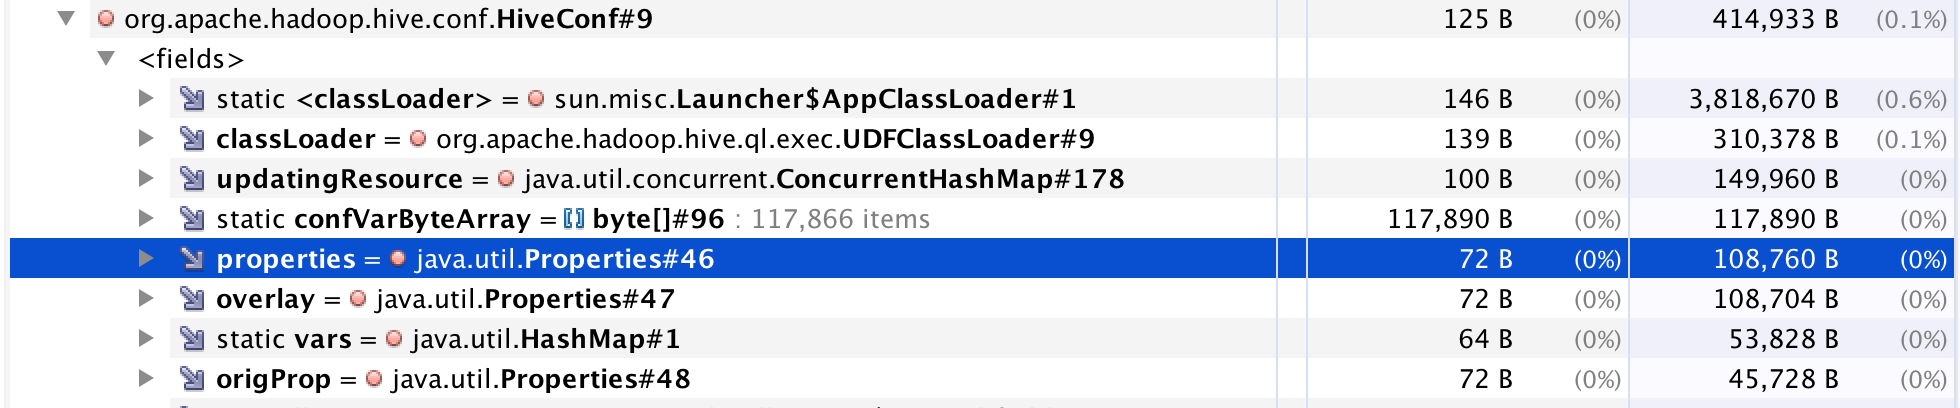
\includegraphics[width=150mm, keepaspectratio]{figures/hiveconf_orig.png}
	\centering
	\caption{Before using HiveConfProperties}
\end{figure}

\subsection{Memory win by the change}
\begin{figure}[H]
	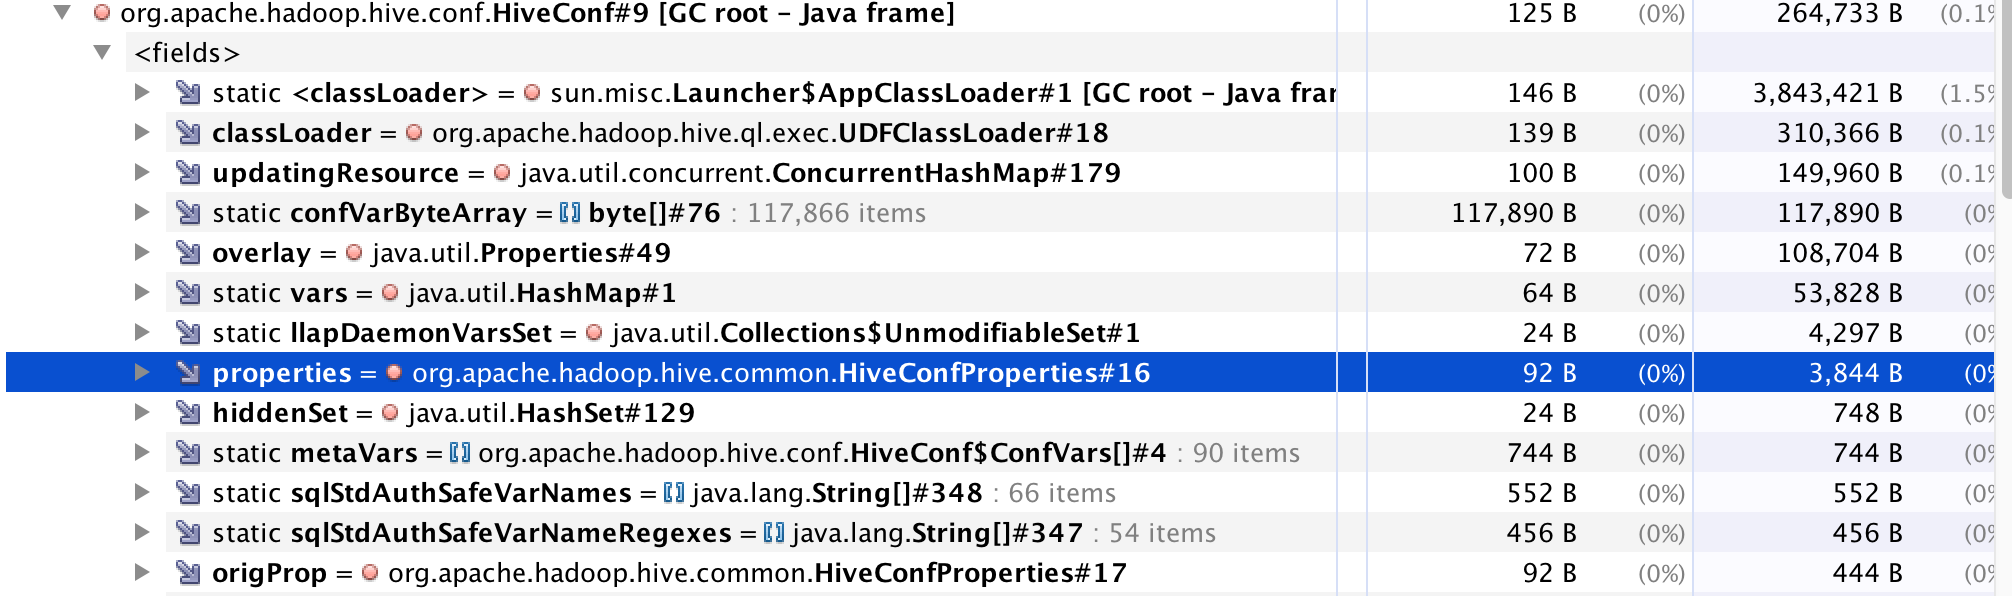
\includegraphics[width=150mm, keepaspectratio]{figures/hiveconf_interned.png}
	\centering
	\caption{After using HiveConfProperties}
\end{figure}

Comparing the heap dumps shows the benefits of interning the Properties in HiveConf. Without the use of HiveConfProperties one configuration object conaining 1910 properties used around 415 Kilobytes. With the use of HiveConfProperties it was reduced to 265 Kilobytes.It is nearly 40\% memory saved for each HiveConf. 

When we use Hive on Spark running with a large number of cores per executor, we have about 10\% of memory overhead due to multiple HiveConfs . This can be reduced significantly using my solution. 

\section{Future work around configuration objects}
The issue I reported is  still ongoing, since tests are needed to see if my patch works correctly in every scenario. I also provided a test class, which needs to be expanded, to cover all the scenarios a Properties object can be used by HiveConf. 

Hadoop also has an implementation of the Configuration class, called JobConf. These objects are also present in HS2 and causes memory overhead the same way as HiveConf does. There is an open source Jira that was intended to solve the duplication without getting \textit{ConcurrentModificationException}, but the memory problem was not resolved just prevented throwing the exception \cite{hive-jobconf}. The solution I provide for HiveConf could also be used for getting rid of the duplication in JobConf.
\chapter{Evaluation}
In this thesis, I learned about the Apache Hadoop ecosystem, especially Hive and the memory constraints and issues it faces. I went through the lifecycle of a query and identified the main parts of compilation and execution. Using this information I provided measuring points to build a model about the memory usage of HiveServer2. I created a code for measuring memory usage automatically and generating heap dumps for later analysis.

\section{Analyzing heap dumps}
During my work, I analyzed many heap dumps. The first step to understand these, was to get a better insight into Java memory model and management. The model was not as simple as I first thought. Java distinguishes young and old memory and these are further divided into different parts. I also got to know many tools, that I used for analysis to make the detection of memory problems easier. 

\section{Results, open issues}
With the measurement tool I created, I was able to detect the phases when Hive's memory usage increases and investigate the reason behind those. I identified two memory wastes and provided ideas and implementation for fixing those. I also experienced the difficulties of such widely used projects.

\subsection{HDFS-13752: Path memory waste}
One of the issues I identified was the duplication of Strings in HDFS. Although, getting rid of the URIs would provide serious memory benefits for Hive and possibly other components, increasing the complexity of such a low level and ubiquitous part of the platform can have unexpected and bad results. 

However, benchmarking HDFS with and without my patch gave us a positive result: no significant overhead can be detected. Still, the community is very careful with the patch, since it touches the very fundament of the distributed file system (basically how we store the paths of the files in it) and it is hard to detect the real effects of the change. Currently, Hive performance tests are planned, but gaining access to a larger cluster where benchmarks can be run is quite difficult. In the future, I will work on this issue and try to push it in Hadoop, even if the outcome may not be a success.

\subsection{HIVE-20760: Duplication of HiveConfs}
The other memory issue I found was caused by the presence of multiple and nearly identical configuration objects, called HiveConf. These configuration values are basically stored in a HashTable. HiveConfs are created regularly in the code: for example, every session gets its own configuration. Hive on Spark (HoS) also has about 10\% of memory overhead due to the duplication of HiveConfs. 

My idea was to divide the Properties into two parts, so different HiveConfs should use the same "base" if those are identical. This way we can prevent creating different objects with the same content. Implementing my solution caused 40\% memory win for every HiveConf. Testing is still needed to cover all scenarios where a configuration object can be used, and if the patch is ready, the community can review it.

\subsection{Gained experience}
I also learned the basics of working on a huge project like Apache Hive and explore its codebase or debug errors. Working on an open source project also provided many benefits. I gained knowledge from reviews and feedbacks have given by far more experienced people around the world. In the future, I am planning to continue my contribution to Hive and I will try to improve one of the most commonly used open source data warehousing solutions.

% Acknowledgements
%~~~~~~~~~~~~~~~~~~~~~~~~~~~~~~~~~~~~~~~~~~~~~~~~~~~~~~~~~~~~~~~~~~~~~~~~~~~~~~~~~~~~~~
%%----------------------------------------------------------------------------
\chapter*{\koszonetnyilvanitas}\addcontentsline{toc}{chapter}{\koszonetnyilvanitas}
%----------------------------------------------------------------------------

I would like to thank Cloudera Hungary for providing infrastructure and resources for writing my thesis. Especially, I would like thank to the Budapest Hive team for answering my questions and giving all the help they could.

A munka a 2017-1.3.1-VKE-2017-00015 számú projekt keretén belül a Nemzeti Kutatási Fejlesztési és Innovációs Alapból biztosított támogatással, a 2017-1.3. pályázati program finanszírozásában valósult meg.


% List of Figures, Tables
%~~~~~~~~~~~~~~~~~~~~~~~~~~~~~~~~~~~~~~~~~~~~~~~~~~~~~~~~~~~~~~~~~~~~~~~~~~~~~~~~~~~~~~
%\listoffigures\addcontentsline{toc}{chapter}{\listfigurename}
%\listoftables\addcontentsline{toc}{chapter}{\listtablename}


% Bibliography
%~~~~~~~~~~~~~~~~~~~~~~~~~~~~~~~~~~~~~~~~~~~~~~~~~~~~~~~~~~~~~~~~~~~~~~~~~~~~~~~~~~~~~~

\addcontentsline{toc}{chapter}{\bibname}
\bibliography{bib/mybib}

% Appendix
%~~~~~~~~~~~~~~~~~~~~~~~~~~~~~~~~~~~~~~~~~~~~~~~~~~~~~~~~~~~~~~~~~~~~~~~~~~~~~~~~~~~~~~


%\label{page:last}
\end{document}
